\documentclass[12pt,letterpaper,oneside]{report}

\usepackage[T1]{fontenc}        % embedded Type 1 fonts (UNH/ProQuest requirement)
\usepackage[utf8]{inputenc}
\usepackage[margin=1in,bottom=1.25in,footskip=0.5in]{geometry} % UNH: 1in margins, page numbers >= 3/4in from edge
\usepackage[doublespacing]{setspace} % UNH: double-spaced text; floats and footnotes stay single-spaced
\usepackage{graphicx}           % Required for inserting images
\usepackage[dvipsnames]{xcolor}
\usepackage{booktabs}           % professional-quality tables
\usepackage{microtype}          % microtypography
\usepackage{mathtools,amssymb,amsthm,bm,bbm,amsfonts,nicefrac}
\usepackage{multirow,enumitem}
\usepackage{array}              % column specs like >{\displaystyle}, used by the mprog environment
\usepackage[ruled,linesnumbered,vlined,noend,algosection]{algorithm2e} % fast-risk chapter algorithms
\usepackage[american]{babel}
\usepackage[numbers,sort&compress]{natbib}
\usepackage{titlesec}
\usepackage{tikz}
\usepackage{caption}            % For custom caption types, like 'mdp'
\usepackage{thmtools}
\usepackage{thm-restate}        % For restating theorems in the appendix
\usepackage{hyperref,url}       % hyperlinks
\usepackage[noabbrev,capitalize]{cleveref}
\hypersetup{colorlinks=true,citecolor=Blue,linkcolor=black,urlcolor=black}

\usetikzlibrary{automata, positioning, arrows.meta, quotes}
% This creates a new environment called 'mdp' that acts lige a figure
\DeclareCaptionType{mdp}[MDP][List of MDPs]
\crefname{mdp}{MDP}{MDPs}
\Crefname{mdp}{MDP}{MDPs} % For capital letters at start of sentences

%%%%%%%%%%%%%%%%%%%%%%%%%%%%%%%%
% THESIS METADATA
%%%%%%%%%%%%%%%%%%%%%%%%%%%%%%%%
\newcommand{\thesistitle}{Efficient Methods for Risk Aware Decision Making}
\newcommand{\thesisauthor}{Gersi Doko}
\newcommand{\thesismonth}{May}          % UNH: May, September, or December
\newcommand{\thesisyear}{2027}
\newcommand{\defensedate}{\todo{defense date}} % TODO: update with actual defense date

\hypersetup{pdftitle={\thesistitle},pdfauthor={\thesisauthor}}

%%%%%%%%%%%%%%%%%%%%%%%%%%%%%%%%
% LAYOUT (UNH Graduate School thesis manual)
%%%%%%%%%%%%%%%%%%%%%%%%%%%%%%%%
% "CHAPTER 1" over the centered title, ~1.5in from the top of the page
\titleformat{\chapter}[display]
{\normalfont\centering}
{\large\bfseries\MakeUppercase{\chaptertitlename}\ \thechapter}
{1em}
{\LARGE\bfseries}
\titleformat{name=\chapter,numberless}[block]
{\normalfont\centering\LARGE\bfseries}{}{0pt}{}
\titlespacing*{\chapter}{0pt}{0.5in}{0.5in}

\addto\captionsamerican{%
  \renewcommand{\contentsname}{CONTENTS}%
  \renewcommand{\listfigurename}{LIST OF FIGURES}%
  \renewcommand{\listtablename}{LIST OF TABLES}%
  \renewcommand{\bibname}{LIST OF REFERENCES}%
}

% unnumbered chapter that is listed in the table of contents
\newcommand{\frontchapter}[1]{
\chapter*{#1}\phantomsection\addcontentsline{toc}{chapter}{#1}}
\renewcommand{\bibsection}{\frontchapter{\bibname}}

% Operators
\newcommand{\opt}{^{\star}}
\renewcommand{\exp}[1]{\operatorname{exp}\left( #1\right) }
\newcommand{\tr}{^{\mathsf{T}}}
\newcommand{\Real}{\mathbb{R}}
\newcommand{\Nats}{\mathbb{N}}

\DeclareMathOperator{\diag}{diag}

\DeclareMathOperator{\kl}{KL}
\DeclareMathOperator*{\argmin}{arg\,min}
\DeclareMathOperator*{\argmax}{arg\,max}
\DeclarePairedDelimiterXPP\expect[2]{\mathbb{E}_{#1}}[]{}{#2}%
\newcommand{\Ex}[1]{\expect*{}{#1}}
\newcommand{\Exp}[2]{\expect*{#1}{#2}}
\newcommand{\E}[1]{\mathbb{E}\left[\, #1 \,\right]} % mpemath (fastcvar) version, takes an argument

% Define risk operators
\newcommand{\risko}{\psi}
\DeclareMathOperator{\varo}{VaR}
\DeclareMathOperator{\cvaro}{CVaR}
\DeclareMathOperator{\conco}{ConC}
\DeclareMathOperator{\oceo}{C}
\DeclareMathOperator{\gento}{GEnT}
\DeclareMathOperator{\fdivo}{FDIV}
\DeclareMathOperator{\evaro}{EVaR}
\DeclareMathOperator{\ermo}{ERM}
\DeclareMathOperator{\ess}{ess}
\DeclareMathOperator{\expectile}{Expectile}
\DeclareMathOperator{\ubsr}{S}

\newcommand{\PiHR}{\Pi_{\mathrm{HR}}}
\newcommand{\PiHD}{\Pi_{\mathrm{HD}}}
\newcommand{\PiAD}{\Pi_{\mathrm{AD}}}
\newcommand{\PiD}{\Pi_{\mathrm{D}}}
\newcommand{\PiR}{\Pi_{\mathrm{R}}}

\newcommand{\Po}{\mathbb{P}}
\renewcommand{\Pr}[1]{\Po\left[ #1 \right]}
\renewcommand{\P}[1]{\Pr{#1}}
\newcommand{\risk}[1]{\psi \left[#1\right]}
\newcommand{\riskd}[2]{\psi_{#1} \left[#2\right]}
\newcommand{\erm}[2]{\ermo_{#1} \left[#2\right]}
\newcommand{\var}[2]{\varo_{#1} \left[#2\right]}
\newcommand{\cvar}[2]{\cvaro_{#1} \left[#2\right]}
\newcommand{\conc}[1]{\conco \left[#1\right]}
\newcommand{\oce}[1]{\oceo \left[#1\right]}
\newcommand{\gent}[2]{\gento_{#1}  \left[#2\right]}
\newcommand{\fdiv}[2]{\fdivo_{#1}  \left[#2\right]}
\newcommand{\evar}[2]{\evaro_{#1} \left[#2\right]}
\newcommand{\ind}[1]{\bm{1}_{#1}}  % Indicator function

\newcommand{\quant}{{\mathfrak{q}}}

% new utility functions
\newcommand{\uvar}{u_{\mathrm{V}}}
\newcommand{\ucvar}{u_{\mathrm{C}}}
\newcommand{\uevar}{u_{\mathrm{E}}}

\DeclareMathOperator{\conv}{cnv}   % convexified function
\DeclareMathOperator{\cl}{cl}      % closure of the function
\newcommand{\conj}{^{\ast}}
\newcommand{\conjconj}{^{\ast\ast}}

% ROIL chapter (from mpemath.sty)
\newcommand{\eps}{\varepsilon}
\DeclareMathOperator{\ext}{ext}   % extreme points
\newcommand{\subjectto}{\operatorname{subject\, to} &}
\newcommand{\minimize}[1]{\operatorname*{minimize}_{#1} &}
\newcommand{\maximize}[1]{\operatorname*{maximize}_{#1} &}
\newenvironment{mprog}{
\begin{array}{>{\displaystyle}c>{\displaystyle}l>{\displaystyle}l}}{
\end{array}}
\newcommand{\stc}{\\[1ex] \subjectto}
\newcommand{\cs}{\\[1ex] & }

% fast-risk chapter (from fastcvar/main.tex and its mpemath.sty)
\DeclareMathOperator{\ER}{DR}
\DeclareMathOperator{\qvar}{QuickVaR}
\DeclareMathOperator{\ews}{EWS}
\DeclareMathOperator{\tvaro}{TVaR}
\newcommand{\tvar}[2]{\tvaro_{#1} \left[#2\right]}
\SetKwInOut{Input}{Input}
\SetKwInOut{Output}{Output}
\IncMargin{2em}

%%%%%%%%%%%%%%%%%%%%%%%%%%%%%%%%
% THEOREMS
%%%%%%%%%%%%%%%%%%%%%%%%%%%%%%%%
\theoremstyle{plain}
\newtheorem{theorem}{Theorem}[section]
\newtheorem{proposition}[theorem]{Proposition}
\newtheorem{lemma}[theorem]{Lemma}
\newtheorem{corollary}[theorem]{Corollary}
\theoremstyle{definition}
\newtheorem{definition}[theorem]{Definition}
\newtheorem{assumption}[theorem]{Assumption}
\theoremstyle{remark}
\newtheorem{remark}[theorem]{Remark}
\newtheorem{example}[theorem]{Example}

% -- comment commands
\newcommand{\mm}[1]{\textcolor{red}{(MP:\ #1)}}
\newcommand{\gersi}[1]{\textcolor{blue}{(GD:\ #1)}}
\newcommand{\todo}[1]{\textcolor{orange}{(TODO:\ #1)}}
\newcommand{\cc}{\bgroup\color{ForestGreen}\let\ccnext=}

% compile only some chapters while drafting
% \includeonly{chapters/introduction}

\begin{document}

%%%%%%%%%%%%%%%%%%%%%%%%%%%%%%%%
% PRELIMINARY PAGES (roman numerals; title page counted as i but unnumbered)
%%%%%%%%%%%%%%%%%%%%%%%%%%%%%%%%
\pagenumbering{roman}
% !TEX root = ../main.tex
% UNH title page: counted as page i, but no page number appears
\thispagestyle{empty}
\begin{center}
  \singlespacing
  \vspace*{0.5in}
  {\large\bfseries \thesistitle\par}
  \vfill
  By\par
  \vfill
  {\large \thesisauthor\par}
  \medskip
  B.S. in Computer Science, University of New Hampshire, 2022\par
  M.S. in Computer Science, University of New Hampshire, 2025\par
  \vfill
  DISSERTATION\par
  \vfill
  Submitted to the University of New Hampshire\par
  in Partial Fulfillment of\par
  the Requirements for the Degree of\par
  \vfill
  Doctor of Philosophy\par
  in\par
  Computer Science\par
  \vfill
  \thesismonth, \thesisyear\par
\end{center}
\clearpage

% !TEX root = ../main.tex
% UNH: optional; include when registering copyright through ProQuest
\vspace*{\fill}
\begin{center}
  \singlespacing
  ALL RIGHTS RESERVED\par
  \textcopyright\thesisyear\par
  \thesisauthor\par
\end{center}
\clearpage
   % optional
% !TEX root = ../main.tex
% UNH committee page: titles exactly as in the Graduate Catalog; non-UNH members list their affiliation
\newcommand{\committeemember}[3]{%
  \par\noindent\hspace*{0.3\textwidth}\parbox[t]{0.7\textwidth}{#1\\ #2\\ #3}\par\vspace{2em}}

\noindent This dissertation has been examined and approved in partial fulfillment of the requirements for the degree of Doctor of Philosophy in Computer Science by:

\vfill
\begingroup
\singlespacing
\committeemember{Marek Petrik, \emph{Doctoral Advisor}}{Associate Professor of Computer Science,}{University of New Hampshire}
\committeemember{\todo{name}}{\todo{title},}{\todo{affiliation}}
\committeemember{\todo{name}}{\todo{title},}{\todo{affiliation}}
\committeemember{\todo{name}}{\todo{title},}{\todo{affiliation}}
\committeemember{\todo{name}}{\todo{title},}{\todo{affiliation}}
\endgroup
\vfill
\hfill On \defensedate
\vfill
\noindent Approval signatures are on file with the University of New Hampshire Graduate School.
\clearpage

% !TEX root = ../main.tex
% UNH: optional
\vspace*{\fill}
\begin{center}
  For Navi, Moose, and Jojo.\\
  My family, and friends.
\end{center}
\vspace*{\fill}
\clearpage
  % optional
% !TEX root = ../main.tex
\frontchapter{ACKNOWLEDGMENTS}

Firstly\cc{ GRAMMAR: "Firstly I" -> "Firstly, I" (comma after introductory word; also consider "First," to pair with "Lastly,", though the two are not strictly parallel)} I would like to thank my family, friends and especially my German Shepard\cc{ TYPO: "Shepard" -> "Shepherd" (the breed is German Shepherd)} Navi for their support and encouragement throughout my graduate career. I am very fortunate to be surrounded by a strong base of support and love that has allowed me to pursue my goals and dreams. I am grateful for their patience and understanding during the long hours of work and study.

If it was\cc{ GRAMMAR: "If it was not for" -> "If it were not for" (subjunctive; or "Were it not for")} not for optimal stopping and its introduction to me at the end of my undergraduate career in fall of 2021\cc{ GRAMMAR: "in fall of 2021" -> "in the fall of 2021" (missing article)} by Dr. Marek Petrik, I would not have pursued this line of research. His passion and knowledge for\cc{ GRAMMAR: "knowledge for this field" -> "knowledge of this field" (knowledge takes "of"; "passion for" is fine)} this field\cc{ GRAMMAR: "field which" -> "field, which" (non-restrictive clause needs a comma before "which"; closing comma after "love" also needed if the clause is kept as an aside)} which I too have come to love has\cc{ GRAMMAR: "has been" -> "have been" (compound subject "passion and knowledge" is plural)} been a source of inspiration and motivation for me. His patience and mentorship have truley\cc{ TYPO: "truley" -> "truly"} transformed me to the point where I cannot remember what I was like before I met him.

Thank you to my collaborators, both here at UNH, abroad, and at other institutions, for their contributions to this work and for their support and camaraderie throughout this process. I am grateful for the opportunity to work with such talented and dedicated individuals. Thank you especially to Dr. Jia Lin Hau for your\cc{ GRAMMAR: "Thank you especially to Dr. Jia Lin Hau for your frequent discussions" -> "...for his frequent discussions" or "Thank you especially, Dr. Hau, for your..." (the sentence names Dr. Hau in the third person, so "your" is a person shift; also "especially to" reads slightly oddly, consider "especially to ... for")} frequent discussions and feedback.

Lastly, I would like to thank my committee members, Dr. Marek Petrik, \todo{committee} for their guidance, support and feedback throughout this process.

This journey has been the most rewarding thing in my life, and I am grateful to be given the opportunity to learn, work and grow here at UNH.

% UNH: dissertations must acknowledge all funding sources (Graduate School awards and external grants)
\todo{grants?}
Additional financial support for this work as well as those works contained within it has been provided by the...\cc{ LATEX: "..." -> \verb|\dots| (placeholder ellipsis; the sentence is unfinished and needs the funder names, see the FUNDING comment below)}\cc{ FUNDING: the fastcvar paper (\cref{ch:fast-risk}) acknowledges NSF grants 2144601 and 2218063, possible wording: "provided by the National Science Foundation under grants 2144601 and 2218063." The ROIL paper and the primal/cdf-var drafts name no funding, so check with Marek whether the ROIL and ETC work had other grants, and add any UNH Graduate School awards or fellowships (the UNH manual requires all funding sources to be acknowledged).}


\tableofcontents
\clearpage\phantomsection\addcontentsline{toc}{chapter}{\listtablename}
\listoftables
\clearpage\phantomsection\addcontentsline{toc}{chapter}{\listfigurename}
\listoffigures

% UNH: the abstract is the last preliminary page, right before the text
% !TEX root = ../main.tex
\frontchapter{ABSTRACT}

\begin{center}
  {\bfseries \thesistitle\par}
  by\par
  \thesisauthor\par
  University of New Hampshire, \thesismonth, \thesisyear\par
\end{center}

Reinforcement Learning is a large area of active research that broadly studies how to make sequential decisions over time. This field is widely varied in its specialties and applications. This work focuses on understanding and broadening the understanding related to risk sensitive reinforcement learning. We build on the existing literature in three key ways. First we propose and solve a new formulation for the Inverse Reinforcement Learning problem. Second we answer an open question about the possibility to find an algorithm which can provably optimize the Conditional Value at Risk of a policy in the space of risk levels. Third we introduce a novel approach to compute risk measures such as Value at Risk and Conditional Value at Risk in expected linear time.

We propose and solve a novel formulation for the Inverse Reinforcement Learning (IRL) problem which frames it as an adversarial game between a policy and a reward function. We show that many existing methods can be cast in this framework, and we provide a new algorithm which solves the optimization as an LP. Unlike existing methods which estimate an expert occupancy frequency directly our method avoids this and instead optimizes over a set of all consistent experts. This allows us to perform well in the offline regime where data comes from a different policy than the experts. We then extend this framework to handle suboptimal experts.

Prior work~\cite{Hau2023DP,Durand2025} has shown that existing methods in risk sensitive reinforcement learning can fail to converge to an optimal policy in certain environments. In this work we purpose conditions on risk measure to enable convergence using standard RL procedures. We also describe a disutility based approach for understanding why some risk measures such as $\cvaro$ can fail to converge. We show that there is a fundamental limitation to these risk measures which prevents them from being optimized in the space of risk levels. \todo{come back after this paper abstract finished}

Finally, we present a novel algorithm which computes risk measure such as Value at Risk and Conditional Value at Risk in expected linear time. This is a logarithmic improvement over existing methods which rely on sorting their inputs. We then demonstrate the effectiveness of our approach numerically on synthetic data and observe a near order of magnitude speed up over existing methods. We generalize our approach to other risk measures which can be optimized as an optimization over a polymatroid. Our solutions are  available publicly at \url{https://github.com/RiskAverseRL/RiskMeasures.jl}.


%%%%%%%%%%%%%%%%%%%%%%%%%%%%%%%%
% TEXT (arabic numerals, starting at 1)
%%%%%%%%%%%%%%%%%%%%%%%%%%%%%%%%
\clearpage
\pagenumbering{arabic}

% !TEX root = ../main.tex
\chapter{Introduction}\label{ch:intro}

The field of machine learning develops algorithms that can perform tasks without being explicitly programmed to do so. Reinforcement learning(RL) is a subfield of machine learning that studies how machines may be trained to perform well in environments they were not explicitly programmed to operate in~\cite{Sutton1998}. This process is summarized typically in a ``loop'' of observing the state of a system, taking an action, and receiving a reward.

In the process of making decisions in real life we often stop and consider possible outcomes of our actions, then take the action which corresponds with the best outcome. This process of evaluating the future possible states of the world and making decisions which maximize those future values is exactly the purpose of RL.

In this work we will primarily focus on specific contributions to the field of risk sensitive reinforcement learning, which has additional considerations for the ``risk'' of outcomes. Consider a doctor deciding what drugs to prescribe patients with a certain ailment. What dose should be prescribed? What are the possible side effects? How likely is it to aid the patient? Could it possibly harm them? These are all questions which add a layer of complexity to the decision process.

\section{Outline}

\todo{describe}

% !TEX root = ../main.tex
\chapter{Preliminaries}\label{ch:prelims}

\section{Markov Decision Processes}

\section{Risk Measures}

\section{Risk Sensitive RL}

% !TEX root = ../main.tex
\chapter{Robust Offline Imitation Learning}\label{ch:roil}

% UNH: a chapter based on a paper must state your role and how it relates to the other chapters
% ---- ported from github.com/GersiD/ChebyshevROIL paper/RIRL_NHT.tex (RLC); reshape as needed ----
% paper abstract:
We study the problem of imitation learning via inverse reinforcement learning where the agent attempts to learn an expert's policy from a dataset of collected state, action tuples. We derive a new Robust model-based Offline Imitation Learning method (ROIL) that mitigates covariate shift by avoiding estimating the expert's occupancy frequency. Frequently in offline settings, there is insufficient data to reliably estimate the expert's occupancy frequency and this leads to models that do not generalize well. Our proposed approach, ROIL, is a method that is guaranteed to recover the expert's occupancy frequency and is efficiently solvable as an LP. We demonstrate ROIL's ability to achieve minimal regret in large environments under covariate shift, such as when the state visitation frequency of the demonstrations does not come from the expert.

\section{Introduction}

\emph{Imitation learning} seeks to compute an optimal policy in a Markov decision process~(MDP) without knowing the reward function. Instead, one only has access to a set of demonstrations performed by a domain expert~\cite{chang2021mitigating, Panaganti2023, Spencer2021, Rashidinejad2022}. Imitation learning promises techniques that can learn to act well in environments where describing an appropriate reward function may be challenging or impractical. Robotics, medicine, and autonomous driving are examples of problem domains that can benefit greatly from more reliable imitation learning algorithms. 

Inverse Reinforcement Learning~(IRL), or apprenticeship learning, is a common approach to imitation learning~\cite{abbeel2004, ziebart2008maximum,fu2018learning}. IRL often leverages the environment's dynamics, modeled as an MDP, to efficiently mimic the observed policy of the expert~\cite{arora2021survey}. The environment's dynamics may be known a priori~\cite{Syed2008, lacotte2019} or estimated from data~\cite{finn2016guided,Ho2016,chang2021mitigating}. An important strength of IRL algorithms is that they can learn to mimic experts quite well even with remarkably little data. However, most IRL algorithms can be very sensitive to the state distribution in the training data. If the distribution of states present in the dataset does not follow the expert's occupancy frequency---a phenomenon known as \emph{covariate shift}---the IRL algorithm may compute a policy that is much worse than the expert's policy. 

In this paper, we propose ROIL, a new approach to IRL that is particularly resistant to any covariate shift. In particular, ROIL allows for data with a state distribution that does not follow the expert's occupancy frequency. Most existing algorithms are sensitive to covariate shifts because, in some form, they reduce to matching the expert's state occupancy frequency. In comparison, ROIL attempts to recover the set of plausible expert policies from the training data and compute a policy that minimizes the regret with respect to this set of experts. With an appropriate choice of modeling assumption, we show that ROIL can be formulated as a convex optimization problem and solved using mature solvers.

There are several reasons why the expert demonstration data may not be sampled according to the true occupancy frequency. First, the expert's initial state distribution may differ from the initial state distribution when the learned policy is deployed. Second, the expert may focus on providing pedagogic demonstrations that focus on the most challenging parts of the state space~\cite{cakmak2012algorithmic,hadfield2016cooperative,Brown2018b}. Third, the demonstrations may not even form a trajectory but instead consist of disconnected state-action pairs. Finally, the state distribution of the demonstrations may differ simply due to sampling and model errors and inconsistencies. Thus, the demonstrations may not be representative of the expert's true policy. As a result, one must be careful in formalizing the IRL problem to make it tractable.

To better illustrate the importance of covariate shift, consider the following extreme example. In an MDP with a small state space and the ability to jump between states, the expert provides a single demonstration for each state showing the optimal actions. Behavior cloning algorithms, which reduce imitation learning to a classification problem, will recover the optimal policy given that the classification bias is general enough. Yet, surprisingly, common IRL algorithms based on the same scheme as LPAL (Linear Programming Apprenticeship Learning)~\cite{Syed2008} or GAIL (Generative Adversarial Imitation Learning)~\cite{Ho2016} can fail to recover a good policy, as we show below. ROIL, on the other hand, recovers the optimal policy even in this extreme setting while preserving most of the benefits of the low sample complexity of IRL. %\gersi{revisit last}

As with most IRL algorithms, ROIL seeks to minimize the regret given the expert's demonstrations for the worst-case plausible reward function. However, ROIL departs significantly from existing IRL algorithms in that it does not directly use the estimate of the expert's occupancy frequency. As a result, ROIL cannot be seen as matching the expert's feature frequencies, which is a popular view of existing IRL techniques~\cite{abbeel2004,Syed2008,Ho2016}. In contrast, ROIL uses the training data to construct a robust set of plausible expert policies and minimizes the regret of the computed policy in the context of this set. 

The remainder of the paper is organized as follows. \Cref{sec:preliminaries} describes the background in MDPs and IRL necessary to introduce ROIL. Then, in \cref{sec:optimization-formulation}, we describe our general framework, analyze its basic properties, propose an optimization algorithm, and discuss several practical extensions. \Cref{sec:theoretical-analysis} analyzes ROIL's guarantees and limitations theoretically and compares them with prior work. Finally, in \cref{sec:experimental-results}, we analyze ROIL numerically and compare it with relevant algorithms. 

\section{Preliminaries}\label{sec:preliminaries}\cc{ TODO: move this section into the Preliminaries chapter (\cref{ch:prelims}). Note that the label sec:preliminaries is also defined in the Preliminaries section of \cref{ch:fast-risk}, so the Cref to it in the roadmap paragraph above currently points to that chapter instead.}

Before describing the underlying MDP framework and formally defining the IRL objective, we define the basic notation we use in the paper. We use calligraphic letters to denote sets and a tilde to denote random variables. We also adopt the standard convention that $\mathcal{A}^{\mathcal{B}}$ represents the set of all functions from a set $\mathcal{B}$ to a set $\mathcal{A}$ and treat vectors as a function from indexes to real numbers. Finally, the sets $\Real$ and $\Real_+$ represent real and non-negative numbers respectively. 


%This introduction is not meant to be exhaustive, but rather to provide the reader with the necessary background to understand the rest of the paper.
%Much of the MDP material comes from~\cite{Puterman1994}.
%For a more in-depth treatment of the IRL setting we refer the reader to~\cite{abbeel2004}.

% \paragraph{Markov Decision Processes}

We assume that the domain can be modeled as a \emph{Markov Decision Process}~\cite{Puterman1994} with a finite number of states $\mathcal{S} = \left\{ 1, \dots , S \right\}$ and a finite number of actions $\mathcal{A} = \left\{ 1, \dots , A \right\}$. The transition probability function $p\colon \mathcal{S} \times \mathcal{A} \to \Delta^{\mathcal{S}}$, where $\Delta^{\mathcal{S}} = \left\{ x\in \Real_{+}^S \mid \sum_{s\in \mathcal{S}} x_s =1 \right\}$ is the probability simplex over the elements of the set $\mathcal{S}$. The reward function $r\opt \colon \mathcal{S} \times \mathcal{A} \to \Real$ represents the reward obtained in each transition. We assume that the initial distribution over $p_0\in \Delta^S$ satisfies that $p_0 > 0$.

A solution to an MDP is a \emph{policy}. In this work, we restrict our attention to \emph{stationary randomized} and \emph{deterministic} policies. The set of deterministic policies is $\Pi_{\mathrm{D}}= \mathcal{A}^{\mathcal{S}}$ and the set of randomized policies is $\Pi_{\mathrm{R}} = {\left(\Delta^{\mathcal{A}}\right)}^{\mathcal{S}}$. Note that deterministic policies are a special case of randomized policies. 

%We consider the $\gamma$-discounted infinite horizon objective with $\gamma \in [0,1)$. The infinite-horizon discounted return of a policy $\pi \in \Pi$ and a reward $r \in \mathcal{R}$ is denoted by $\rho(\pi, r)$. 

%The set of deterministic policies is $\Pi_D= \mathcal{A}^{\mathcal{S}}$ and the set of randomized policies is $\Pi_{\mathrm{R}} = {\left(\Delta^{\mathcal{A}}\right)}^{\mathcal{S}}$. The set of all policies is $\Pi = \Pi_{\mathrm{R}} \cup \Pi_D$.

The objective in this work is the $\gamma$-discounted infinite horizon objective with $\gamma \in [0,1)$. We denote the infinite-horizon discounted \emph{return} of a policy $\pi \in \Pi$ and a reward $r \in \mathcal{R}$ is denoted by 
\[
  \rho(\pi, r)
  \;=\; \lim_{T\to\infty} \mathbb{E}^{\pi, p_0} \left[   \sum_{t=0}^{T} \gamma^t r(\tilde{s}_t,\tilde{a}_t) \right], 
\]
where the superscript on the expectation indicates that $\tilde{s}_0 \sim p_0$ and $\tilde{s}_{t+1} \sim p(\cdot | \tilde{s}_t,\tilde{a}_t)$, and $\tilde{a}_t \sim \pi(\cdot | \tilde{s}_t)$.  The return $\rho$ is parameterized by the reward because, in the IRL setting, the reward is uncertain. 


It will be convenient to treat functions that map states and actions to real numbers as vectors, such as the reward function $r\opt \in \Real^{SA}$. We also use $P_{\pi} \in \Real_+^{S \times S}$ where $P_{\pi}(s,\cdot) = \sum_{a \in \mathcal{A}} p(\cdot | s, a) \pi(a|s)$ and $r_{\pi}\in \Real^S = \sum_{a \in \mathcal{A}}r(s, a)\pi(a|s)$ to represent the transition probability matrix and reward vector respectively for each policy $\pi\in \Pi$. Similarly, $P_a$ and $r_a$ represent the transition probability matrix and a reward vector respectively for each action $a\in \mathcal{A}$.

An important and well-known fact that we use is the relation between the occupancy frequencies and policies. In particular, for each policy $\pi\in\Pi_{\mathrm{R}}$ there exists an occupancy frequency $u^{\pi}\in \Real^{\mathcal{S}\times \mathcal{A}}$ such that $\rho(\pi, r) = r_{\pi}\tr u^{\pi}$. The space of occupancy frequencies for all $\pi\in \Pi_{\mathrm{R}}$
is denoted as $\mathcal{U}$ and satisfies~\cite[Section~6.9]{Puterman1994}:
\begin{equation} \label{eq:definition-u}
  \mathcal{U}
  \; =\; 
\left\{ u^{\pi} \mid  \pi \in \Pi \right\}
\; =\;
\Bigl\{ u\in \Real^{SA}_{+} \mid \sum_{a\in \mathcal{A}} (I - \gamma\cdot P\tr_a) \cdot u(\cdot, a) = p_0 \Bigr\}.
\end{equation}
Finally, for each $u\in \mathcal{U}$, one can construct a policy $\pi_u$ such that $u^{\pi} = u$~\cite[Theorem~6.9.1]{Puterman1994} as
\begin{equation}\label{eq:policy-construction}
\pi_u(a|s) \; =\;  \frac{u(s,a)}{\sum_{a' \in \mathcal{A}} u(s,a')}, \qquad \forall s\in \mathcal{S}, a\in \mathcal{A}.
\end{equation}
The policy $\pi_{\mathrm{u}}$ is well-defined because $p_0 > 0$ guarantees that $\sum_{a\in \mathcal{A}} u(s,a) > 0$ for each $s\in \mathcal{S}$. 

%\paragraph{Inverse Reinforcement Learning}

With the definitions above, we are now ready to describe the general IRL framework~\cite{abbeel2004,Syed2008,Ho2016}. Recall that the main goal is to learn to act in an environment without knowing the true reward function $r\opt$. Instead, we have access to transition data generated from an expert's policy $\pi_{\mathrm{e}} \in \Pi_{\mathrm{D}}$. To simplify the exposition, we assume that the expert follows a deterministic policy and we discuss generalizations to randomized policies in \cref{sec:optimization-formulation}. The IRL algorithm has access to a dataset  \( \mathcal{D} = {(t_i, s_i, \pi_e(s_i))}_{i=1}^D \), where the states may or may not be selected sequentially from state trajectories.

To generalize from a small set of demonstrations, IRL algorithms typically rely on a feature function $\phi\colon \mathcal{S} \times \mathcal{A}\to \Real^k$ that assigns $k$ features to each state and action~\cite{abbeel2004,Syed2008,Brown2018a,lacotte2019,chang2021mitigating,jonnavittula2021know,arora2021survey}. The features $\phi$ represent important characteristics of the state-action pairs that may be part of the demonstrator's reward function. We can represent our features with a feature matrix $\Phi \in \Real^{SA\times k}$ where each row represents the features of a specific state and action. Linear IRL algorithms assume that rewards can be expressed as a linear combination of state and action features. Formally, the set $\mathcal{R} \subseteq \Real^{SA}$ of \emph{feasible rewards} is defined as
\begin{equation} \label{eq:r-defintion}
  \mathcal{R} = \left\{ \Phi w \mid  w\in \mathcal{W} \right\}, \quad
  \text{where} \quad
  \mathcal{W} = \left\{ w \in \Real^k \mid \| w \|_1 \le 1 \right\}. 
\end{equation}
The $L_1$ norm in the definition of $\mathcal{W}$ serves to normalize $w$ because optimal policies are invariant to the scale of the rewards~\cite{abbeel2004,Syed2008}. 

Most IRL algorithms adopt the following scheme. The true reward $r\opt$ is unknown but is assumed to satisfy that $r\opt \in \mathcal{R}$. Algorithms as varied as LPAL~\cite{Syed2008}, GAIL~\cite{Ho2016}, and MILO~\cite{chang2021mitigating} seek to compute a policy that minimizes the worst-case regret with respect the expert's policy. In its essence the regret minimization problem is usually formalized as
\begin{equation} \label{eq:IRL_formulation}
\min_{\pi \in \Pi} \max_{r \in \mathcal{R}} \; \Bigl( \rho(\hat{\pi}_{\mathrm{e}}, r) - \rho(\pi, r) \Bigr).
\end{equation}
Here, $\hat{\pi}_{\mathrm{e}}$ is the empirical estimate of the expert policy $\pi_{\mathrm{e}}$ constructed from the dataset $\mathcal{D}$.

The conceptual optimization in~\eqref{eq:IRL_formulation} is impractical because the optimization over $\pi$ is non-convex and computationally challenging. Instead, using the correspondence between policies and occupancy frequencies in~\eqref{eq:policy-construction}, LPAL and related algorithms solve the following surrogate optimization problem:
\begin{equation} \label{eq:irl-formulation-u}
  \min_{u\in \mathcal{U}} \max_{r\in \mathcal{R}} \, \left(\hat{u}_{\mathrm{e}}\tr r - u\tr r \right)
  \; =\; 
  \min_{u\in \mathcal{U}} \, \left\| (\hat{u}_{\mathrm{e}} - u)\tr \Phi \right\|_{\infty},
\end{equation}
where the equality follows because $L_{\infty}$ is the dual norm to the $L_1$ norm used in the definition of $\mathcal{W}$.

The value $\hat{u}_{\mathrm{e}}$ in \eqref{eq:IRL_formulation} represents the \emph{empirical} estimate of $u_{\mathrm{e}}\opt$ constructed as
\begin{equation} \label{eq:definition_u_hat}
  \hat{u}_e(s,a)
  \;=\; \chi \cdot \sum_{(t, s',a') \in \mathcal{D}} \gamma^t \cdot  \mathbbm{1}\left\{s=s' \wedge\; a=a'\right\},
\end{equation}
where $\chi$ is a normalization factor chosen to guarantee that $1\tr \hat{u}_{\mathrm{e}} = (1-\gamma)^{-1}$. In practice, it is common to estimate the \emph{feature counts} $\hat{u}_{\mathrm{e}}\tr \Phi$ directly rather than estimating $\hat{u}_{\mathrm{e}}$.

Some IRL algorithms, like GAIL, add other regularization terms to the scheme in~\eqref{eq:irl-formulation-u} and substitute different definitions for the reward set $\mathcal{W}$~\cite{Ho2016}. In this work, we focus on the fundamental properties and trade-offs of this formulation and leave more complex extensions for future work.

An important limitation of the formulation in~\eqref{eq:irl-formulation-u} is that it relies on estimating the expert's occupancy frequency $\hat{u}_{\mathrm{e}}$ well. Because the occupancy frequency represents the frequency of \emph{both} states and actions it is very sensitive to the initial distribution and covariate shifts in state distributions which may often arise in imitation learning settings. As discussed in the introduction, the expert may focus on difficult states when performing the demonstrations or have a behavioral state visitation policy that dictates what states to visit. In the remainder of the paper, we build on~\eqref{eq:irl-formulation-u} to address its sensitivity to the initial distribution and state distribution of the provided dataset, thereby achieving better off-policy performance. 

%Non-sequential, in this context, means that the dataset $\mathcal{D}$ may have state, action tuples where $s_{t+1}$ is not distributed accoding to $P(\cdot | s_t, a_t)$. 


% The core of most IRL algorithms is to solve the following optimization problem which minimizes the tobust regret with respect to the occupancy frequency of the expert. 
% \begin{equation} \label{eq:IRL_formulation}
% 	\min_{\pi \in \Pi} \max_{r \in \mathcal{R}} \; (\rho(\pi_{\mathrm{e}}, r) - \rho(\pi, r)),
% \end{equation}
% where $\Pi$ is the set of all policies with $\pi_{\mathrm{e}} \in \Pi$, $\mathcal{R}$ is the set of all reward functions, and $\rho$ is the $\gamma$ discounted 
% \section{Optimization Formulation}\label{sec:optimization-formulation}

% We assume that the true reward function can be written as a linear combination of the features $\Phi$ which are known.

% We will focus on the robust IRL problem, where there is an inner maximization over $\Pi$, see \cref{sec:optimization-formulation}.

\section{ROIL Formulation}\label{sec:optimization-formulation}

% We begin by stating the general formulation of the IRL problem.
% \begin{equation}
% 	\min_{\pi \in \Pi} \max_{r \in \mathcal{R}} \; (\rho(\pi_{\mathrm{e}}, r) - \rho(\pi, r)),
% \end{equation}
% where $\Pi$ is the set of all policies with $\pi_{\mathrm{e}} \in \Pi$, $\mathcal{R}$ is the set of all reward functions, and $\rho$ is the $\gamma$ discounted infinite horizon
% return of a policy given some reward function. This setting is useful for domains where the reward function is hard to define, 
% but features and demonstrations are available. Such domains include robotics, medicine, and autonomous driving. 
% We will focus on the robust IRL problem, where there is an inner maximization over $\Pi$, see \cref{sec:optimization-formulation}.

In this section, we describe and justify ROIL and study its computational properties; we defer the analysis of its approximation errors to \cref{sec:theoretical-analysis}. First, we describe the foundations of the approach in \cref{sec:basic-formulation} and then outline several modifications that reduce ROIL's conservativeness and improve its performance in \cref{sec:incorp-addit-constr}. We conclude the section with a visualization of ROIL as a Chebyshev center problem, which offers additional insights into its performance in \cref{sec:geom-intu-reduct}.  


\subsection{Basic Formulation}
\label{sec:basic-formulation}

Similarly to the standard IRL schema outlined in~\eqref{eq:irl-formulation-u}, ROIL also adopts a principled robust optimization perspective and minimizes the worst-case regret.  The main idea is to compute a policy $\pi\in \Pi$ that minimizes regret with respect to the worst-case plausible expert's policy $\pi_{\mathrm{e}} \in \Pi_{\mathrm{R}}(\mathcal{D})$ and a reward function $r\in \mathcal{R}$. Formally, the basic ROIL optimization problem is as follows:
\begin{equation}
\label{eq:robust_IRL_formulation}
\min_{\pi \in \Pi_{\mathrm{R}}(\mathcal{D})}  \max_{\pi_{\mathrm{e}} \in \Pi_{\mathrm{R}}(\mathcal{D})} \max_{r \in \mathcal{R}} \,
\left(\rho(\pi_{\mathrm{e}}, r) - \rho(\pi, r)\right).
\end{equation}
Here, $ \Pi_{\mathrm{R}}(\mathcal{D}) \subseteq \Pi_{\mathrm{R}}$ represents the set of all policies consistent with $\mathcal{D}$ and are defined as 
%
\begin{equation} \label{eq:consistent-policies}
\Pi_{\mathrm{R}}(\mathcal{D}) = \left\{ \pi \in \Pi_{\mathrm{R}} \mid \pi(a|s) = 1, \, \forall (s,a) \in \mathcal{D} \right\}.
\end{equation}

If the expert demonstrations in $\mathcal{D}$ are constructed from a deterministic policy, then that policy must be contained in~\eqref{eq:consistent-policies}. However, when the expert's policy is randomized, the construction in~\eqref{eq:consistent-policies} may exclude the expert policy from $\Pi_{\mathrm{R}}(\mathcal{D})$. We discuss how the definition can be extended to account for randomized policies in \cref{sec:incorp-addit-constr}. 

Before describing an efficient formulation for solving ROIL, we discuss its benefits compared with the generic IRL scheme in~\eqref{eq:IRL_formulation}. Recall that $\hat{u}_{\mathrm{e}}$, constructed in \eqref{eq:definition_u_hat},  depends on the initial state distribution which may lead to large errors when the demonstration and execution state distributions differ. Instead, ROIL uses the training data to construct the set $\Pi_{\mathrm{R}}(\mathcal{D})$---which is independent of the state distribution---and minimizes regret to all consistent expert policies. 

Next, we show that the ROIL optimization problem in~\eqref{eq:robust_IRL_formulation} can be reduced to a linear program with a polynomial size. It may be surprising that such a reduction is possible since ROIL's objective involves maximizing a non-concave bilinear function. We derive this reduction using the occupancy-based formulation, similar to existing IRL algorithms. A key part of the formulation is a set of occupancy frequencies $\Upsilon$ that are consistent with expert demonstrations defined for $c\in \Real^{SA}$ as 
%
\begin{equation}\label{eq:consistent-occupancies}
  \Upsilon = \left\{ u \in \mathcal{U} \mid c\tr u = 0  \right\},
  \quad
  \text{ where }
  \quad
  c(s,a) =
  \begin{cases}
    1 &\text{if  }
        (s,a) \notin \mathcal{D} \wedge
        \exists a'\in \mathcal{A}, (s, a') \in \mathcal{D}, \\
    0 & \text{otherwise}.
  \end{cases}
\end{equation}

% Now we illustrate the robust IRL learning problem as an optimization problem over the policy and reward space. Then we simplify it using occupancy frequencies
% and the fact that the reward function is linearly realizable by $\Phi$. This allows us in the following section to formulate the problem as a linear program.

% Recall the IRL objective.
% \begin{equation}
% 	\min_{\pi \in \Pi} \max_{r \in \mathcal{R}}  \, (\rho(\pi_{\mathrm{e}}, r) - \rho(\pi, r)),
% \end{equation}


The following lemma shows that the set of occupancy frequencies constructed in~\eqref{eq:consistent-occupancies} is exactly the set of frequencies of policies that are consistent with the dataset. 
\begin{restatable}{lemma}{lemmaOccupancyExistance}
\label{lemma:occ_freq_matching}
If $\mathcal{D}$ is generated by a deterministic policy $\pi \in \Pi_{\mathrm{D}}$. Then
\[
  u \in \Upsilon
  \qquad \Leftrightarrow \qquad
  \left(u = u^{\pi},\;  \exists \pi \in \Pi_{\mathrm{R}}(\mathcal{D})\right).
\]
\end{restatable}
Please see the proof in \cref{sec:appendix_proofs}.

We now outline the main step in constructing a linear program formulation for solving ROIL. As \cref{lemma:occ_freq_matching} shows,  maximizing over the policy space is equivalent to maximizing over the occupancy frequency space. Then, using the fact that $\rho(\pi,r) = r\tr u^{\pi}$ and the representation of $\mathcal{R}$ in~\eqref{eq:r-defintion}, we can reformulate~\eqref{eq:robust_IRL_formulation} to
%
\begin{equation} \label{eq:roil-occupancy}
    \min_{u \in \Upsilon} \max_{r \in \mathcal{R}} \max_{v \in \Upsilon} \, (v- u )\tr  r
    \; =\; 
    \min_{u \in \Upsilon} \max_{w \in \mathcal{W}} \max_{v \in \Upsilon} \, (v - u)\tr \Phi w.
\end{equation}
%

Solving the formulation in~\eqref{eq:roil-occupancy} directly is challenging because it involves maximizing a non-concave bilinear function in both $w$ and $v$. To turn this optimization into a tractable convex optimization problem, we take the following steps. The maximization over $w$ maximizes a convex function $w \mapsto \max_{v \in \Upsilon} \, (v - u)^T \Phi w$. Therefore, there exists an optimal $w$ in one of the extreme points of $\mathcal{W}$, leading to the following equivalent formulation:
\begin{equation} \label{eq:extreme-points-reformulated}
    \min_{u \in \Upsilon} \max_{w \in \ext(\mathcal{W})} \, \left(-u\tr \Phi w + \max_{v \in \Upsilon} v\tr \Phi w \right) .
\end{equation}
The set $\mathcal{W}$ is an $L_1$-norm ball. The number of its extreme points is linear in the number of features, and we can enumerate them to obtain the following linear program:
\begin{equation} \label{eq:roil-basic-lp}
    \begin{mprog}
        \minimize{t \in \Real, u \in \Real^{SA}} t
        \stc t \geq -u\tr \Phi w +  b(w),\quad \forall w \in \ext(\mathcal{W}),
        \cs u\in \Upsilon,
    \end{mprog}
  \end{equation}
  where $b(w) = \max_{v \in \Upsilon} v\tr \Phi  w$. Note that the constraints $u\in \mathcal{U}$ defined in~\eqref{eq:definition-u} are linear and $b(w)$ can be computed by solving a linear program or an MDP.

From the discussion above and the epigraph formulation~\cite{Boyd_Convex_Optimization}, we get the following theorem that states the correctness of the linear program formulation.
% \begin{restatable}{prop}{roilLp}
\begin{proposition}
    \label{thm:roil_lp}
    Let $u\opt$ be optimal in~\eqref{eq:roil-basic-lp}. Then, $\pi_{u\opt}$ constructed in~\eqref{eq:policy-construction} is an optimal $\pi$ in~\eqref{eq:robust_IRL_formulation}.
\end{proposition}
% \gersi{TODO add proof} marek: the discussion is good enough as a proof , imo
% \end{restatable}

% \paragraph{Visual Representation of ROIL}


\subsection{Extensions}
\label{sec:incorp-addit-constr}

An important strength of ROIL is its flexibility. The basic ROIL formulation makes no assumptions except that actions in $\mathcal{D}$ are distributed according to the expert's policy. It also does not make any assumptions about the state distribution or the optimality of the expert's policy.
In this section, we discuss several simple techniques that can be used to incorporate additional assumptions about the data in $\mathcal{D}$ that help to compute less conservative solutions.

First, we can make ROIL less conservative by restricting the generic reward set $\mathcal{R}$ when computing the regret. If the expert's policy $\pi_{\mathrm{e}}$  is close to optimal, it is sufficient to consider only a subset of $\mathcal{R}$ restricted to rewards that are consistent with the near-optimality of $\pi_{\mathrm{e}}$. That is, we can solve \eqref{eq:roil-occupancy} with $\mathcal{W}_{\mathrm{e}}^\tau \subseteq \mathcal{W}$ defined as
\begin{equation} \label{eq:prune-r}
  \mathcal{W}_{\mathrm{e}}^\tau\;:=\;
  \left\{ w\in \mathcal{W} \mid \hat{u}_{\mathrm{e}}\tr \Phi w + \tau \ge  \max_{u\in \mathcal{U}} u\tr \Phi w  \right\},
\end{equation}
where $\tau \ge 0$ represents the allowed sub-optimality of the expert's policy $\pi_{\mathrm{e}}$. It is important to emphasize that the optimality of a policy is insensitive to the choice of the initial distribution. In practice, we adapt \eqref{eq:roil-basic-lp} to solve
\begin{equation} \label{eq:roil-prune-lp}
    \begin{mprog}
        \minimize{t \in \Real, u \in \Real^{SA}} t
        \stc t \geq -u\tr \Phi w +  b(w),\quad \forall w \in \mathcal{W}_{\mathrm{e}}^\tau,
        \cs u\in \Upsilon.
    \end{mprog}
  \end{equation}
We solve this optimization problem by first collecting $m$ samples $w\in \mathcal{W}_{\mathrm{e}}^{\tau}$ from a uniform distribution and then choose $\tau$ in~\eqref{eq:prune-r} appropriately to retain $10\%$ of the samples.


A second option for reducing the conservativeness of ROIL is to suppose that the expert's demonstrations are close to being on-policy.
% That is, the demonstrations visit states with \emph{approximately} the same frequency as when following the policy when generating trajectories.
Then, one can use $\mathcal{D}$ to estimate $\hat{u}_{\mathrm{e}} \approx u_{\mathrm{e}}\opt $ and consider the set $\hat{\Upsilon}_{\epsilon}$ defined as
%
\begin{equation}
\label{linf_constraint}
\hat{\Upsilon}_{\epsilon}
\;=\;
\left\{ u \in \Upsilon \mid \| (\hat{u}_{\mathrm{e}} - u)\tr \Phi \|_{\infty} \le \eps \right\}.
\end{equation}
This set represents all policies that are consistent with the expert's demonstrations and also have occupancy frequencies that are close to the observed expert data. One can estimate $\epsilon$ by solving
\begin{equation}\label{eq:minimal-epsilon}
\epsilon \; =\;  \eta \cdot \min_{u\in \mathcal{U}}
\| (\hat{u}_{\mathrm{e}} - u)\tr \Phi \|_{\infty}, 
\end{equation}
where $\eta \ge 1$ is some constant. %Another option is to choose $\epsilon$ from domain information combined with finite-sample bounds for estimating occupancy frequencies~\cite{abbeel2004}.
The linear program in~\eqref{eq:roil-basic-lp} can be easily adapted to handle the restricted set $\hat{\Upsilon}_e$ by redefining $b(w) = \max_{v \in \hat{\Upsilon}_e} v\tr \Phi  w$. 

Finally, we discuss how to extend ROIL to account for randomized expert demonstrations. In such scenario, the constraint $c\tr u = 0$ must be replaced by a constraint $u_{s,a} / \sum_{a'\in \mathcal{A}} u(s,a') - \hat{\pi}_{\mathrm{e}}( s,a ) \le \epsilon, \forall s\in \mathcal{S}, a\in \mathcal{A}$ for some appropriately chosen $\epsilon$ and an estimate $\hat{\pi}_{\mathrm{e}}$ of expert's policy. Using perspective functions, one can readily see that this constraint is convex and does not increase the computational complexity of this formulation.

% As is often the case we have introduced 4 dual variables in out LP which have unique interpretations. These variables are $\alpha_i, \hat{\alpha}_i \in \Real$ and $\beta_i, \hat{\beta}_i \in \Real^S$. The $\alpha$ dual variables represent an importance weight of $c$ which is our constraint vector~\ref{eq:consistent-occupancies}. The $\beta$ vectors are a feature-based state value function, from this point of view the first two constraints ensure that the absolute difference between our occupancy frequency's feature expectation and that of the models is as close can be.

% To solve the inner maximization we assume that the constraints on $\Upsilon$ are linear or can be coerced into linear constraints.
% \begin{equation}
%     \begin{mprog}
%         \maximize{v \in \Real^{SA}} v\tr r_i
%         \stc A\tr v = p_0
%         \cs v \geq 0
%         \cs g_j(v) \leq 0
%     \end{mprog}
% \end{equation}

% Let $u_{\mathrm{R}}(\eps)$ be the minimizer of \ref{eq:new_robust_IRL} when the set $\Upsilon$ is defined as in \ref{linf_constraint}, and let $f_{\mathrm{R}}(\eps)$ be the objective value achieved by $u_{\mathrm{R}}(\eps)$.
% Let $f_t$ be the objective value of 
% %
% \[\max_{r\in\mathcal{R}} r\tr (u_{\mathrm{e}} - u_r(\eps))\]
% %
% then 
% %
% \[f_t \leq f_{\mathrm{R}}(e_t)\]
% \[f_{\mathrm{R}}(\eps_t) = \min_{u \in \Upsilon(\eps_t)} \max_{v \in \Upsilon(\eps_t)} \lvert\lvert \Phi\tr (v-u) \rvert\rvert_\infty\]
% \[\geq \min_{\mu \in \mathcal{U}} \lvert\lvert \Phi\tr (u_{\mathrm{e}} - \mu) \rvert\rvert_\infty \geq f_t\]


% A second possible extension that can reduce the pessimism of ROIL is to restrict $\pi$ to $\Upsilon$. That is, we seek only policies consistent with the expert's demonstration. Using the Chebyshev center formulation described in \cref{sec:geom-intu-reduct}, it can be readily seen that such a restriction does not affect the relative regret attained by ROIL. With this restriction, the optimization problem in~\eqref{eq:extreme-points-reformulated} becomes
% \[
%  \min_{u \in \Upsilon} \max_{w \in \ext(\mathcal{W})} \, \left(-u\tr \Phi w + \max_{v \in \Upsilon} v\tr \Phi w \right),
% \]
% which can also be solved using a linear program with only minor modifications. Putting the two modifications described above together turn~\eqref{eq:roil-basic-lp} to the following linear program:
% \begin{equation} \label{eq:roil-improved-lp}
%     \begin{mprog}
%         \minimize{t \in \Real, u \in \Real^{SA}} t
%         \stc t \geq -u\tr \Phi w +  \hat{b}_{\epsilon}(w),\quad \forall w \in \ext(\mathcal{W}),
%         \cs u\in \hat{\Upsilon}_{\epsilon},
%     \end{mprog}
%   \end{equation}
%   where $\hat{b}_{\epsilon}(w) = \max_{v \in \hat{\Upsilon}_{\epsilon}} v\tr \Phi  w$.




\subsection{Discussion and Visualization}
\label{sec:geom-intu-reduct}

We now discuss a connection between ROIL and the geometric problem of computing the Chebyshev center of a convex set. This connection helps to elucidate what conditions make ROIL tractable and offers an intuitive way of visualizing ROIL and its relationship with other IRL algorithms. 

In~\eqref{eq:r-defintion}, we define the set $\mathcal{W}$ in terms of an $L_1$ ball. However, this set could be defined in terms of any norm $\| \cdot \|$ as $\mathcal{W} = \left\{ w\in \Real^k \mid \| w \| \le 1 \right\}$.  For any norm, there exists a \emph{dual norm} $\| \cdot  \|_{\star}$ defined as \( \| x\|_{\star}\; =\;  \sup_{y \neq 0} \, \nicefrac{y \tr x}{\|y\|} . \)~\cite{Horn2013}.
The dual to an $L_p$ norm ($p \ge 1$) is an $L_q$ norm such that $\nicefrac{1}{p} + \nicefrac{1}{q} = 1$. Using the definition of a dual norm, the ROIL optimization problem in~\eqref{eq:roil-occupancy} can be represented as
\begin{equation} \label{eq:robust_IRL_formulation_L1}
\min_{u \in \mathcal{U}} \max_{v \in \Upsilon} \, \|(v - u)\tr \Phi\|_{\star}.
\end{equation}
The following proposition states the correctness of \eqref{eq:robust_IRL_formulation_L1} and follows from the discussion above. 
% \begin{restatable}[Consistent Regret]{proposition}{chebeyshevRegret}
\begin{proposition}
\label{thrm:chebeyshevRegret}
Suppose that $u\opt$ is optimal in~\eqref{eq:robust_IRL_formulation_L1} with $\| z  \|_{\star} = \| z \|_{\infty}$ for $z\in \Real^k$. Then $\pi_{u\opt}$, as constructed in~\eqref{eq:policy-construction}, is an optimal $\pi$ in~\eqref{eq:robust_IRL_formulation}.
% \end{restatable}
\end{proposition}
% \gersi{need proof}

The optimization problem in~\eqref{eq:robust_IRL_formulation_L1} is equivalent to computing the \emph{Chebyshev center} of the set $\Upsilon$ with respect to the norm defined by $\| \cdot  \|_{\infty}$. The Chebyshev center is a point that minimizes the distance to the most distant point in the set $\Upsilon$. \Cref{fig:visual_representation_of_ROIL} visualizes the Chebyshev center for an MDP with two features. The red polygon represents the set $\mathcal{U}$ and the green polygon represents the set $\Upsilon$; the points correspond to deterministic policies.
%Note that the extreme points of $\Phi\tr \Upsilon$ are also deterministic policies in $\mathcal{U}$ but do not constitute extreme points of $\Phi\tr \mathcal{U}$.

% In other words, the Chebyshev center is the center of the smallest circumscribed $\| \cdot \|_{\infty}$ ball to the set $\Upsilon$. The problem of computing the Chebyshev center has been studied widely in the literature and numerous algorithms have been proposed~\cite{Wu2013, Eldar2008}.

%It is important to note that some authors use the term Chebyshev center to refer to the problem of computing the center of the largest \emph{inscribed} ball~\cite{Boyd_Convex_Optimization} which is related but has different properties.





\begin{figure}
    \centering
    %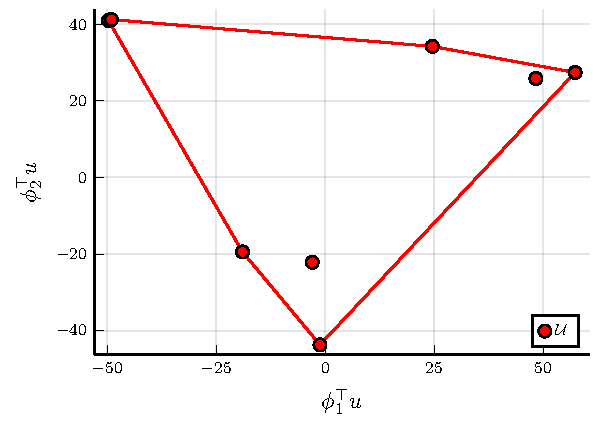
\includegraphics[width=0.45\textwidth]{figs/roil/visual_U.pdf}
    % 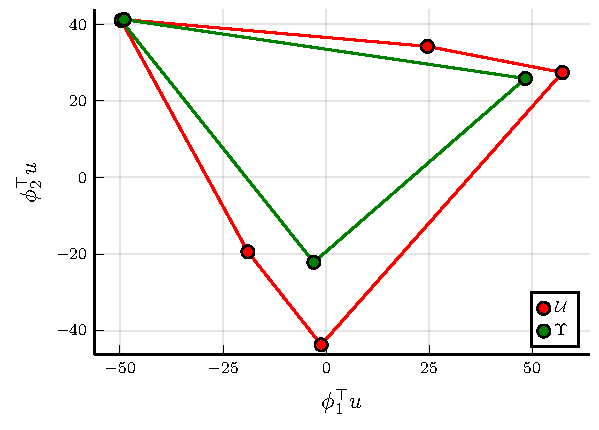
\includegraphics[width=0.35\textwidth]{figs/roil/visual_U_and_Upsilon.pdf}
    % \hspace{0.1\textwidth}
    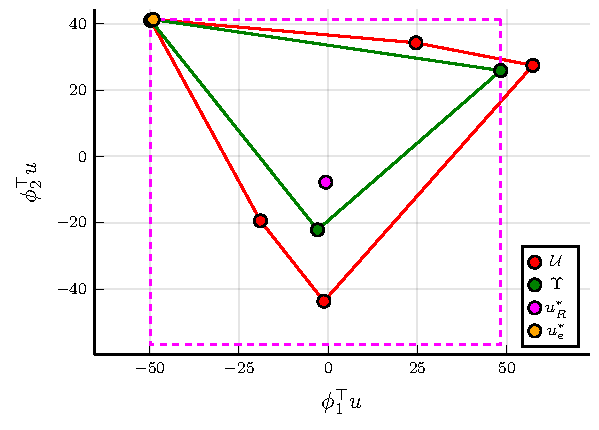
\includegraphics[width=0.45\textwidth]{figs/roil/visual_solve_cheb.pdf}
    %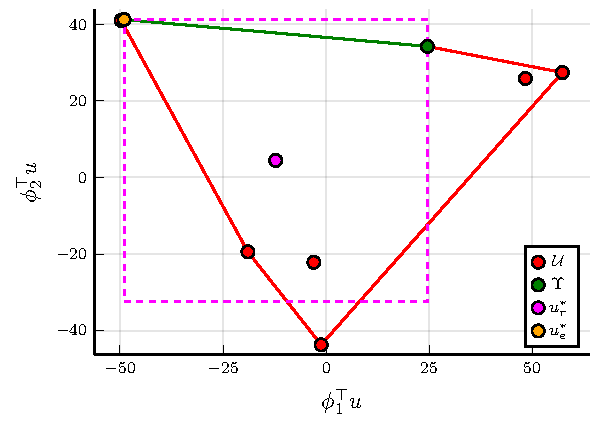
\includegraphics[width=0.35\textwidth]{figs/roil/visual_solve_cheb_outside_upsilon.pdf}
    \caption{Depiction of ROIL solution ($u^*_R$) as a Chebyshev center of the set $\Upsilon$. The dashed line shows the minimum circumscribed  $L_{\infty}$ ball.
%\gersi{Are we sure circumscribed is the right word?}
%https://www.merriam-webster.com/dictionary/circumscribe   definition 2a
    }
    \label{fig:visual_representation_of_ROIL}
\end{figure}


The relationship to the Chebyshev center problem also offers additional computational insights regarding the choice of $\mathcal{W}$. It is known that popular choices of the distance metric $\| \cdot  \|_{\star}$ in computing the Chebyshev center of a polyhedron are NP-hard. One notable exception is when the distance metric $\| \cdot \|_{\star}$ corresponds to the $L_{\infty}$ norm. Since $L_1$ is the dual norm to the $L_{\infty}$ norm, the choice of $L_1$ in the definition of $\mathcal{W}$ is crucial to obtaining a tractable optimization problem~\cite{Wu2013, Eldar2008}.


% optimization problem. In the convex optimization literature,
% ~\eqref{eq:robust_IRL_formulation_L1} is a problem of finding the largest minimum
% distance between the edges of polytopes $\mathcal{U}$ and $\Upsilon$. Also known as the Chebyshev center of $\Upsilon$ with respect to $\mathcal{U}$.
% This problem is known to be NP-hard except for certain cases \gersi{citation needed}.

% For those familiar with prior works done by Syed and Schapire~\cite{Syed2008} this is very similar to LPAL and MWAL.
% However, we show that our formulation is more general and can recover the expert exactly in particular cases.


% \begin{equation}
% \label{linProg}
%     \begin{mprog}
%             \minimize{\sigma, \alpha_i, \hat{\alpha}_i \in \Real, \beta_i, \hat{\beta}_i \in \Real^{S}, u \in \Real^{SA}} \sigma
%             \stc -u\tr \Phi_i - \beta_i\tr p_0 \leq \sigma
%             \cs u\tr \Phi_i - \hat{\beta}_i\tr p_0 \leq \sigma
%             \cs \Phi_i + \alpha_i c + A \beta_i \leq 0
%             \cs -\Phi_i + \hat{\alpha}_i c + A \hat{\beta}_i \leq 0
%             \cs i \in 1 \dots k
%             \cs A\tr u = p_0
%             \cs u \geq 0
%     \end{mprog}
% \end{equation}

\section{Theoretical Analysis}
\label{sec:theoretical-analysis}
% \mm{Things to show:
% 	\begin{enumerate}
% 		\item When each state is present in the dataset, then we can compute a policy that has zero worst-case regret
% 		\item What if there is one state that we have not seen, can we bound the regret then?
% 	\end{enumerate}
%  }

In this section, we turn to a theoretical analysis of ROIL. We study the theoretical guarantees of the quality of the solutions computed by ROIL. In particular, we show that, unlike other popular IRL algorithms, ROIL guarantees to recover the expert's policy when demonstrations for all states are available. We also discuss the limitations that arise from the assumption inherent in ROIL formulations and give an approximation error bound in terms of the approximation error bounds.

First, we show that LPAL and GAIL, popular IRL algorithms, suffer from a surprising weakness. The algorithms may not recover the expert's policy even when given demonstrations of deterministic actions for \emph{every} state in a tabular MDP. While it is not a prevalent scenario in practice, it points out that simply adding more demonstrations is insufficient for these methods. We consider LPAL and GAIL, which can be stated for tabular features $\Phi = I$ as the following optimization problems:
\begin{equation} \label{eq:lpal-gail}
  \min_{u\in \mathcal{U}}\, \| u - \hat{u}_{\mathrm{e}} \|_{\infty},
  \qquad
  \text{and}
  \qquad
  \min_{u\in \mathcal{U}} \, D_{\mathrm{JS}}(u, \hat{u}_{\mathrm{e}}) - \lambda H(\pi^{u}).
\end{equation}
Here, the first optimization problem represents LPAL~\cite{Syed2008} and the second optimization represents GAIL~\cite[eq.~(15)]{Ho2016}. The distance metric $D_{\mathrm{JS}}$ represents the Jensen-Shannon entropy, and $\lambda \ge 0$ is a regularization parameter. The LPAL optimization problem in~\eqref{eq:lpal-gail} follows immediately from~\eqref{eq:irl-formulation-u} by optimizing over the set of occupancy frequencies. For the sake of consistency with ROIL, we assume that $\mathcal{W}$ is chosen as in~\eqref{eq:r-defintion}. This is a superficial difference from the original LPAL derivations that assume that feature weights are non-negative: $\mathcal{W} = \left\{ w\in \Real^k_+ \mid \| w\|_1 \le  1  \right\}$.

\begin{proposition}
LPAL and GAIL as defined in~\eqref{eq:lpal-gail} may not recover $\pi_{\mathrm{e}}$ even when the demonstrations cover the entire state space: $ \left\{ s\in \mathcal{S} \; \mid \; \exists\; a\in \mathcal{A}, \; (s,a) \in \mathcal{D} \right\} = \mathcal{S}$. 
\end{proposition}
We show the proposition by constructing the following example.
% \gersi{Marek I can't figure out how to get the Figures for these examples to line up so while people are reading they can see the examples :(}\mm{that is OK. Let floats be floats and let them float.}
\begin{example} \label{exm:fail-all}
Consider an MDP with two states and transition probabilities depicted in \cref{fig:example-fail-one}. Suppose that $\pi_{\mathrm{e}}(s) = a_1$ for each $s\in \mathcal{S}$.  The occupancy frequency for this policy is $u\opt_{\mathrm{e}} = \left[ \frac{\epsilon + \gamma - 1}{\epsilon(1-\gamma)}, 0, \frac{1}{\epsilon}\right]$. Assume that the dataset $\mathcal{D} = ( (s_1, a_1), (s_2, a_1) )$ represents the demonstrations; note that the state distribution needs to respect the state distribution of $u_{\mathrm{e}}\opt $. The estimated occupancy frequency from this dataset will be $\hat{u}_{\mathrm{e}} = \left[\frac{1}{2(1-\gamma)}, 0, \frac{1}{2(1-\gamma)}\right]$ where the elements correspond to $(s_1, a_1), (s_1, a_2), (s_2,a_1)$. The set of occupancy frequencies in this MDP is
\begin{equation} \label{eq:u-definition-example}
  \mathcal{U}_\xi = \left\{ \xi \cdot \left[\frac{\epsilon+\gamma-1}{\epsilon(1-\gamma)}, 0, \frac{1}{\epsilon}\right] + (1-\xi) \cdot \left[0,1-\epsilon,\frac{\gamma}{1-\gamma}+\epsilon\right] \;\mid\; \xi \in [0,1]\right\},
\end{equation}
because the set of occupancy frequencies of randomized policies can be represented as a convex hull of the frequencies of deterministic policies. One can then readily verify that $u_{\mathrm{e}}\opt $ does not minimize either one of the objectives in~\eqref{eq:lpal-gail} when $\lambda = 0$. Specifically, choosing $\xi = 0.5$ in~\eqref{eq:u-definition-example} achieves minimal loss however one can easily verify $u^\star_{\mathrm{e}} = u_\xi$ when $\xi = 1$. \Cref{fig:loss_of_LPAL_GAIL} depicts the objective functions in~\eqref{eq:lpal-gail} as a function of $\xi$ in~\eqref{eq:u-definition-example}.
\end{example}

\begin{figure}
\centering
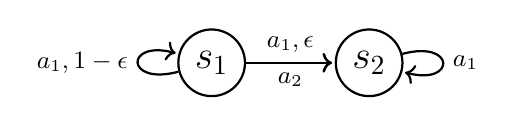
\begin{tikzpicture}[->,shorten >=1pt,auto,node distance=2cm,
thick,main node/.style={circle,draw,font=\sffamily\Large\bfseries}]
\node[main node] (1) {$s_1$};
\node[main node] (2) [right of=1] {$s_2$};
\path[every node/.style={font=\sffamily\small}]
(1) edge [loop left] node {$a_1, 1-\epsilon$} (1)
(1) edge node [below, midway] {$a_2$} (2)
(1) edge node [above, midway] {$a_1, \epsilon$} (2)
(2) edge [loop right] node {$a_1$} (2);
\end{tikzpicture}
\caption{MDP used in \cref{exm:fail-all}. The edge labels denote the actions and the corresponding transition probabilities (if less than 1).}
\label{fig:example-fail-one}
\end{figure}

In contrast with LPAL and GAIL, ROIL is guaranteed to recover the expert's policy when provided with demonstrations for all states as the following proposition states.  
\begin{proposition} \label{expert_recovery}
Suppose that $\left\{ s\in \mathcal{S} \; \mid \; (\cdot,s,\cdot) \in \mathcal{D} \right\} = \mathcal{S}$. Then $u_{\mathrm{e}}\opt $ is the unique minimizer to~\eqref{eq:roil-basic-lp}. %Moreover, with the constraint $u\in \Upsilon$ discussed in \cref{sec:incorp-addit-constr}, $u_{\mathrm{e}}$ is also the unique minimizer.
\end{proposition}   
\begin{proof}
When $\mathcal{D}$ completely covers the states, $\Pi_{\mathrm{R}}(\mathcal{D}) = \left\{ \pi_{\mathrm{e}} \right\}$ and $\Upsilon = \left\{ u_{\mathrm{e}}\opt \right\}$ by \cref{lemma:occ_freq_matching}. One can readily see that $u_{\mathrm{e}}\opt$ attains $0$ objective in~\eqref{eq:roil-basic-lp}, which is optimal because the regret is lower-bounded by $0$. The uniqueness is immediate because $\Upsilon$ is a singleton.
\end{proof}

\begin{figure}
\centering
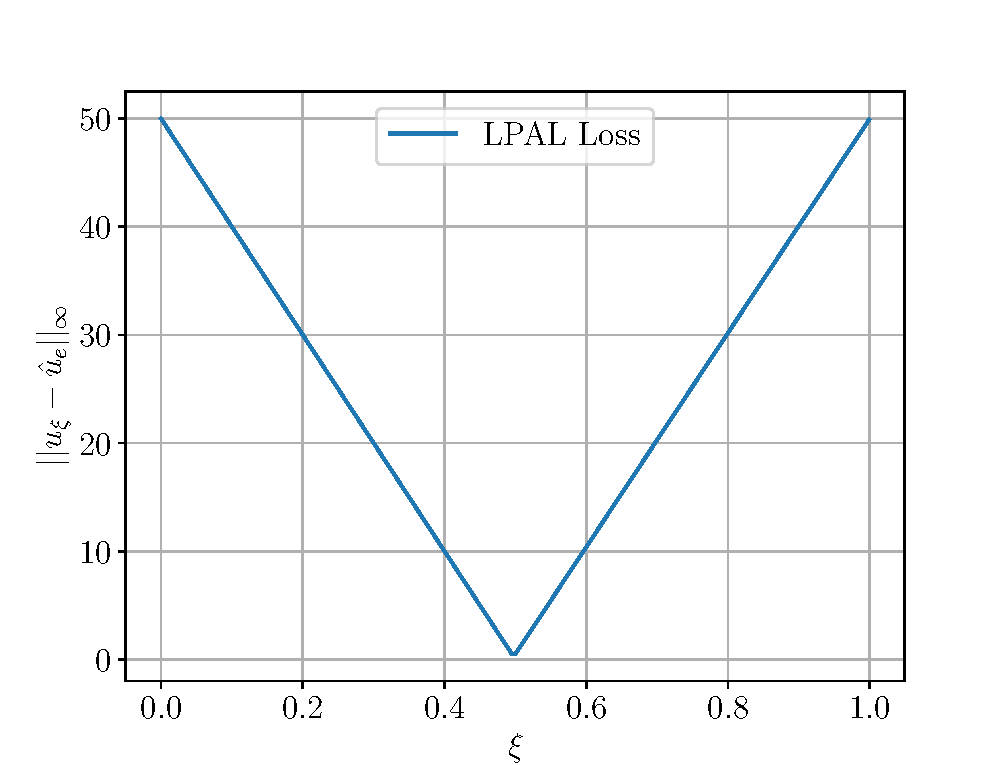
\includegraphics[width=0.35\textwidth]{figs/roil/lpal_loss.pdf}
\hspace{0.05\linewidth}
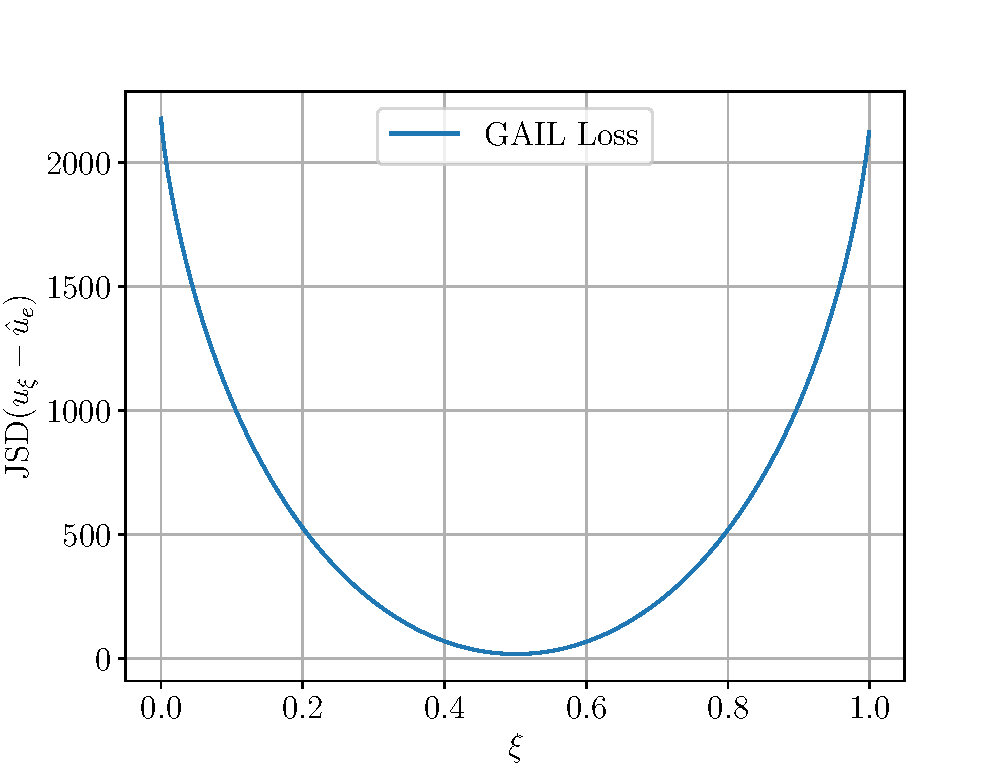
\includegraphics[width=0.35\textwidth]{figs/roil/gail_loss.pdf}
\caption{The loss functions of LPAL and GAIL. Here JSD refers to the Jensen-Shannon Divergence which is the loss function minimized by GAIL when the coefficient of the 
causal entropy term H is zero~\cite{Ho2016}.}
\label{fig:loss_of_LPAL_GAIL}
\end{figure}

\begin{figure}
  \centering
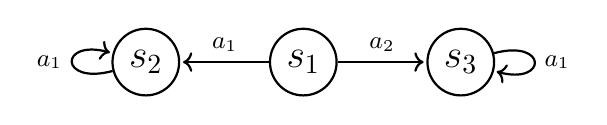
\begin{tikzpicture}[->,shorten >=1pt,auto,node distance=2cm,
            thick,main node/.style={circle,draw,font=\sffamily\Large\bfseries}]

    \node[main node] (1) {$s_1$};
    \node[main node] (2) [left of=1] {$s_2$};
    \node[main node] (3) [right of=1] {$s_3$};

    \path[every node/.style={font=\sffamily\small}]
    (1) edge node [above] {$a_1$} (2)
    edge node [above] {$a_2$} (3)
    (2) edge [loop left] node {$a_1$} (2)
    (3) edge [loop right] node {$a_1$} (3);
\end{tikzpicture}
  \caption{An MDP used in \cref{exm:roil-limitations}.}
  \label{fig:roil-fail}
\end{figure}

Recall that ROIL dispenses with the assumption that the states in the demonstrations $\mathcal{D}$ are distributed according to the occupancy frequency. This assumption makes ROIL appropriate in a broader range of off-policy scenarios than competing IRL algorithms. However, the following result shows the limitations arising from ignoring the state distribution assumption in $\mathcal{D}$. The following example demonstrates that even when all but one state is covered by $\mathcal{D}$, ROIL cannot give any guarantees on the regret of the computed policy. 

\begin{example} \label{exm:roil-limitations}
Consider the deterministic MDP depicted in \cref{fig:roil-fail} where $\mathcal{S} = \{s_1, s_2, s_3\}$, $\mathcal{A} = \{a_1, a_2\}$, $p_0 = [1,0,0]$, and $\Phi = r\opt = [0,0,1,1,-1,-1]$. Here, $r\opt$ is the true reward and vectors are ordered as $(s_1,a_1), (s_1, a_2), (s_2,a_1), \dots $. Assume that the expert follows the optimal policy $\pi_{\mathrm{e}}(s) = a_1, \forall s\in \mathcal{S}$ with an occupancy frequency $u_{\mathrm{e}}\opt  = [1,0,\nicefrac{\gamma}{1-\gamma},0,0,0]$. However, ROIL fails to find this solution even when demonstrations cover all but one state. Consider the dataset $\mathcal{D} = ((s_2, a_1),  \dots, (s_2, a_1))$. The optimal solution to ROIL is $u = [\nicefrac{1}{2},\nicefrac{1}{2},\nicefrac{\gamma}{2(1-\gamma)},0,\nicefrac{\gamma}{2(1-\gamma)},0]$ which is sub-optimal regardless of how well the estimated $\hat{u}_{\mathrm{e}}$ approximated $u_{\mathrm{e}}\opt $. Using the observed data, ROIL has no evidence supporting taking actions $a_1$ or $a_2 $ in the initial state $s_1$.
\end{example} 

\Cref{exm:roil-limitations} exposes a limitation of ROIL but also hints at how to overcome it. Note that occupancy frequency matching methods, like LPAL~\cite{Syed2008}, may do well in \cref{exm:roil-limitations}. This is because LPAL will use the prevalence of the state $s_2$ in $\mathcal{D}$ to deduce that taking action $a_1$ in $s_1$ is preferable to $a_2$. As we discuss in \cref{sec:incorp-addit-constr}, it is easy to extend ROIL to benefit from similar distributional assumptions. The following theorem establishes approximation bounds for ROIL with this assumption. 
\begin{theorem} \label{roilRegretBound}
Suppose that $u_{\mathrm{r}}\opt$ is an optimal solution to~\eqref{eq:roil-basic-lp} with $\hat{\Upsilon}_{\epsilon}$ some $\epsilon>0$ such that $\hat{\Upsilon}_{\epsilon} \neq \emptyset$ and an occupancy frequency estimate $\hat{u}_{\mathrm{e}}$. Then the regret of $\pi_{\mathrm{r}}\opt  = \pi^{u\opt_{\mathrm{r}}}$ is bounded as
\[
 \rho(\pi_{\mathrm{e}}, r) - \rho(\pi_{\mathrm{r}}\opt, r)
\;\leq\;
\| (u_{\mathrm{e}}\opt  - \hat{u}_{\mathrm{e}})\tr \Phi \|_\infty + \eps,
\qquad \forall r\in \mathcal{R}.
\]
Moreover, one can choose $\epsilon$ such that $ \epsilon = \| (u_{\mathrm{e}}\opt  - \hat{u}_{\mathrm{e}})\tr \Phi \|_\infty$.
\end{theorem}
\begin{proof}
The result follows by replacing the worst-case over the $L_1$ ball by its dual norm ($L_{\infty}$), and from the construction of $\mathcal{W}$, and the triangle inequality:
\begin{align*}
\rho(\pi_{\mathrm{e}}, r) - \rho(\pi_{\mathrm{r}}\opt, r)
  &\le  \max_{r\in\mathcal{R}} (u_{\mathrm{e}}\opt  - u_{\mathrm{r}}\opt)\tr r
    = \| (u_{\mathrm{e}}\opt  - u_{\mathrm{r}}\opt)\tr \Phi \|_\infty
    \leq \| (u_{\mathrm{e}}\opt  - \hat{u}_{\mathrm{e}} + \hat{u}_{\mathrm{e}} - u_{\mathrm{r}}\opt)\tr \Phi \|_\infty \\
&\leq \| (u_{\mathrm{e}}\opt -\hat{u}_{\mathrm{e}})\tr \Phi \|_\infty + \| (\hat{u}_{\mathrm{e}} - u_{\mathrm{r}}\opt)\tr \Phi \|_\infty \leq  \| (u_{\mathrm{e}}\opt -\hat{u}_{\mathrm{e}})\tr \Phi \|_\infty + \eps.
\end{align*}
The last inequality follows from the fact that the $u_{\mathrm{r}}\opt  \in \hat{\Upsilon}_{\epsilon}$.
\end{proof}

\Cref{roilRegretBound} shows that when $\| (u_{\mathrm{e}}\opt  - \hat{u}_{\mathrm{e}})\tr \Phi \|_\infty $ is small, then ROIL with the extensions is guaranteed to find a policy that has a small regret to the expert's policy. We also note that \cref{roilRegretBound} essentially matches the error bounds derived for LPAL~\cite{Syed2008}.

%%%%%%%%%%%%%%%%%%%%%%%%%%%%%%%%%%%%%%%

\section{Experimental Results}
\label{sec:experimental-results}


In this section, we study ROIL's behavior numerically on common benchmark problems. We study its performance both on-policy (states distributed according to the \gersi{true expert} policy) and off-policy (states distributed arbitrarily) and compare it with closely related IRL algorithms.

The first domain we use is an instance of the standard grid world problem~\cite{abbeel2004} in which each square is designated a color that represents the feature that is active for the state. The reward is some linear combination of the features for each state. That is, the matrix $\Phi$ represents the state colors and  $r\opt  = \Phi\tr w$ for some $w \in \mathcal{W}$. The features for each action in the state are identical. The agent has a choice of up, down, left, and right as their actions with small noise that takes it to a different neighboring state. The rewards in this domain are generated randomly for each run by sampling $w$ uniformly from $\mathcal{W}$. The expert policy is computed and chosen as the optimal policy for the true (unobserved) reward.

The second domain we use is a driving simulator inspired by \citet{abbeel2004} and \citet{Syed2008} where the agent begins in the bottom row and can go straight up, up and to the left, or up and to the right. At the first row, the actor loops back to the bottom row to simulate a continuous environment. Similarly to the grid world, the driving simulator has some small noise in the transitions. The driving simulator has some motorists on the road, which the actor must avoid, and the left-most and right-most columns are designated as ``offroad'' where the actor receives negative rewards.

To generate on-policy data, we use the standard protocol in which expert demonstrations are trajectories of a policy. To generate off-policy data, we simulate an expert who aims to give uniform coverage of the states. That is, the expert follows a uniform behavior policy  $\pi_b(a|s) = \nicefrac{1}{\lvert \mathcal{A} \rvert}$, which controls the transition dynamics. The uniform policy $\pi_{\mathrm{b}}$ is only used to generate the states in $\mathcal{D}$ and the actions are chosen by the true expert $\pi_{\mathrm{e}}$.

%This off-policy regime makes it difficult to recover the expert for any method that relies solely on $\hat{u_e}$, which is the estimated occupancy frequency given the expert dataset.

We evaluate two versions of ROIL: The basic ROIL makes no assumptions on $\hat{u}_{\mathrm{e}}$ and solves~\eqref{eq:roil-basic-lp}. ROIL-P solves~\eqref{eq:roil-prune-lp}, pruning away reward functions that make $\hat{u}_{\mathrm{e}}$ perform sub-optimally see \cref{eq:roil-prune-lp}. We compare these algorithms with two IRL algorithms: LPAL and GAIL. For consistency with our results, we do not impose the constraint $w \ge 0$ used in the original LPAL formulation~\cite{Syed2008}. For the GAIL implementation, we use the original formulation with $\lambda = 0$; we did not find that $\lambda$ had a significant effect on our results. We also compare it with Naive Behavioral Cloning~(NBC). NBC follows the expert's policy in states that are visited but takes a random action in states that have not been visited.

\begin{figure}
\centering 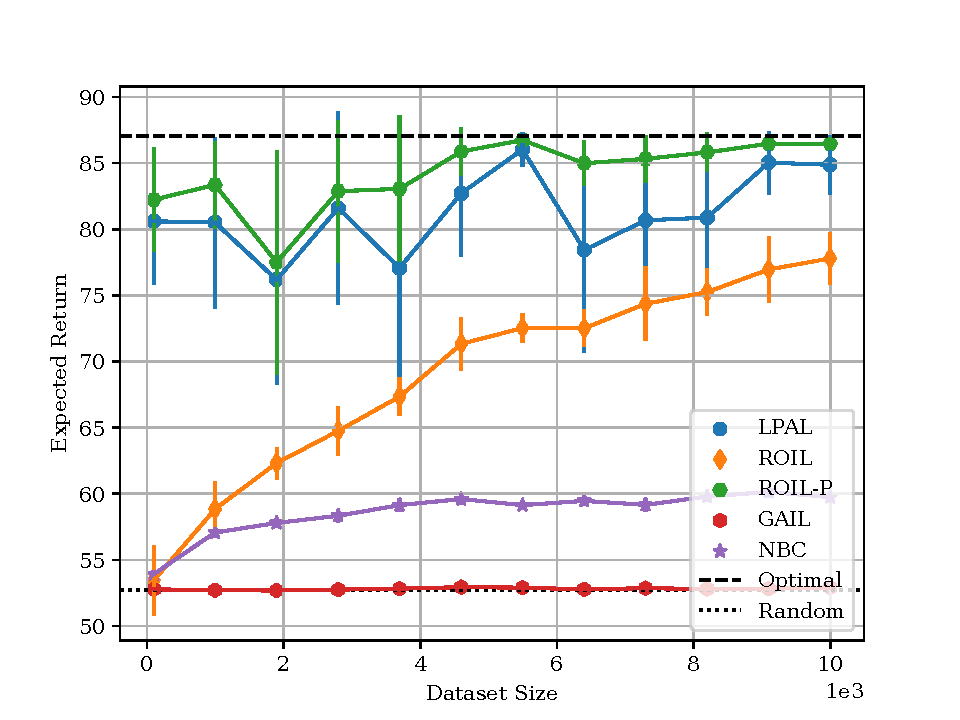
\includegraphics[width=0.49\textwidth]{figs/roil/40x40_gridworld_on_policy_returns.pdf} 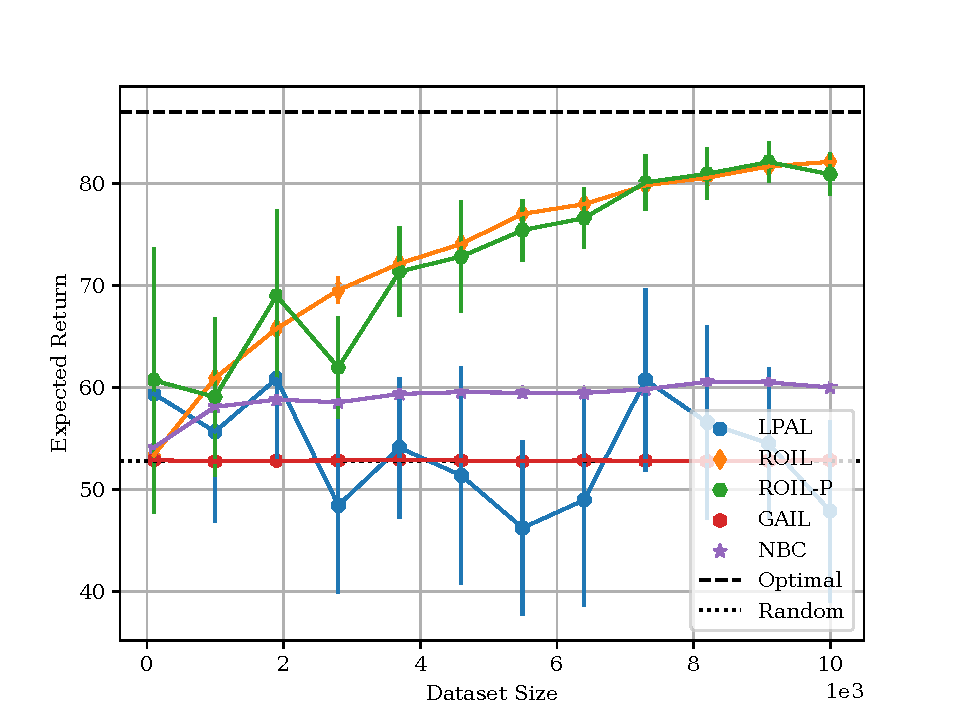
\includegraphics[width=0.49\textwidth]{figs/roil/40x40_gridworld_off_policy_returns.pdf}
\caption{On-policy (left) and off-policy (right) expected return of imitation learning methods on 40x40 grid world for a fixed reward. Higher is better.}
\label{fig:grid-40}
\end{figure}

\Cref{fig:grid-regret,fig:grid-40} depict the performance of multiple IRL methods as a function of the number of samples in the demonstrations. The samples are constructed from trajectories sampled from the domain. Each data point is computed as an average of 10 seeds, and standard error bars are displayed; see the appendix for more details. We do not provide timing data because most of the algorithms are implemented in Python, and the main focus of our methods is for a setting where sample complexity and not computation time are the limiting factors. 

LPAL performs very well on policy in our experiments. This is unsurprising because it matches $\hat{u}_{\mathrm{e}}$, and its estimate improves with increasing samples. However, in the off-policy regime, LPAL and other occupancy frequency matching methods fail to work well because the estimate $\hat{u}_{\mathrm{e}}$ does not necessarily improve with increasing numbers of samples. ROIL, on the other hand, works well in both settings. 

Our experiments demonstrate that ROIL and ROIL-P perform well both on-policy and off-policy. Because ROIL minimizes the worst-case regret, it can be quite conservative when the dataset is small. In comparison, our results confirm that pruning the reward vectors in ROIL-P makes it less conservative and improves its performance significantly. Additional empirical evaluation and discussion of methods described in \cref{sec:incorp-addit-constr} can be found in \cref{sec:experimental_results_revisited}. 

\begin{figure}
\centering 
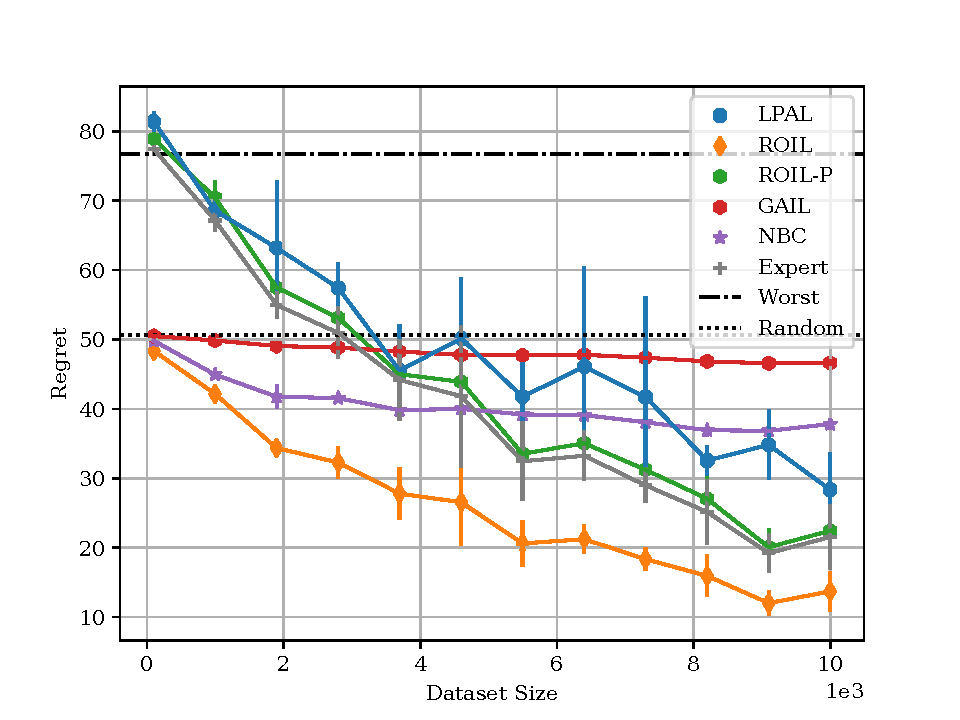
\includegraphics[width=0.45\textwidth]{figs/roil/40x40_gridworld_on_policy_regret_regrets.pdf} 
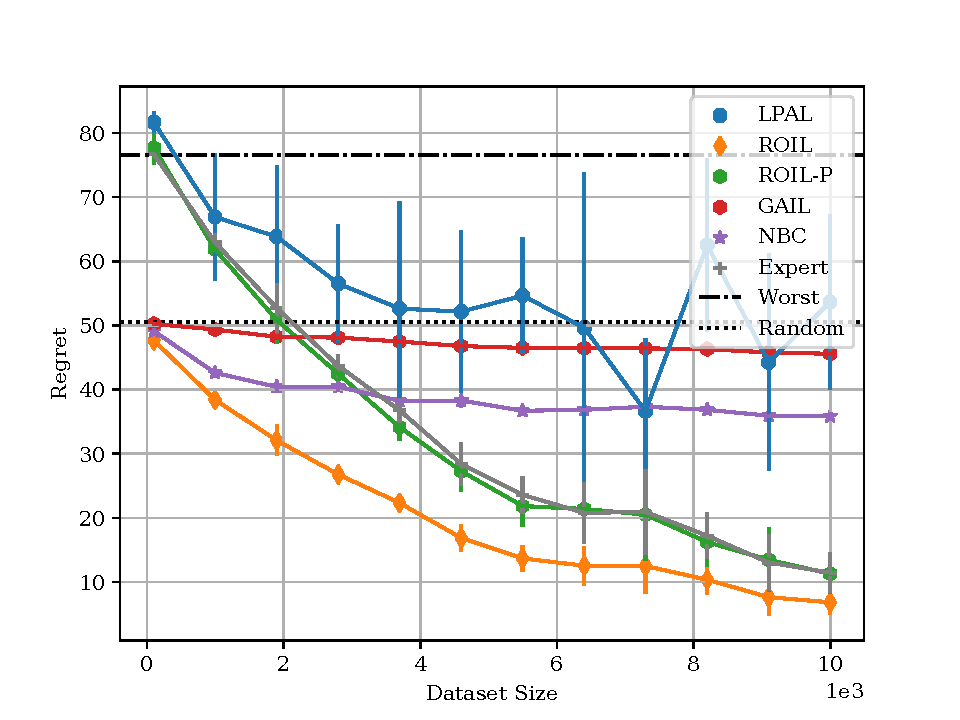
\includegraphics[width=0.45\textwidth]{figs/roil/40x40_gridworld_off_policy_regret_regrets.pdf}
\caption{Robust regret for on-policy (left) and off-policy (right) of imitation learning methods on 40x40 Grid World (lower is better).}
\label{fig:grid-regret}
\end{figure}


%%%%%%%%%%%%%%%%%%%

\section{Conclusion}

We presented a new algorithm for IRL that can handle expert demonstrations gathered from off-policy (or offline) state distributions which may not form a trajectory. This is an important topic that, to the best of our knowledge, has not received sufficient attention in prior work. We proposed ROIL, a principled and flexible framework for this problem. ROIL minimizes the regret concerning the expert's policy and makes minimal assumptions about the data and the expert. However, the framework can be easily extended to a setting in which one makes more assumptions about the expert and the demonstrations generated. We address a surprising weakness with other IRL methods like LPAL and GAIL and provide guarantees on our convergence to the expert policy. 

There are many avenues for future work. ROIL builds on the same ideas as most modern IRL algorithms and can be readily integrated with the improvements developed in recent years~\cite{arora2021survey}. It is important to study whether there are possible refinements of ROIL along the lines described in \cref{sec:incorp-addit-constr} that would significantly impact its performance. We also studied ROIL in a simple tabular setting. Future work should study the best ways to generalize these ideas to large problems with continuous states and actions and non-linear function approximators.

% !TEX root = ../main.tex
\chapter{Extended Time Consistent Risk Measures in MDPs}\label{ch:etc}

% UNH: a chapter based on a paper must state your role and how it relates to the other chapters
\todo{port from \texttt{\textasciitilde/grad/primal/cvar.tex}}

% !TEX root = ../main.tex
\chapter{Computing Monetary Risk Measures in Linear Time}\label{ch:fast-risk}

% UNH: a chapter based on a paper must state your role and how it relates to the other chapters
% ---- ported from ~/grad/fastcvar/main.tex (TMLR); reshape as needed ----
% paper abstract:
Monetary risk measures have gained popularity for expressing decision-makers' risk aversion. Value-at-Risk (VaR) and Conditional-Value-at-Risk (CVaR), in particular, are used commonly for this purpose. This paper proposes new efficient algorithms to compute these risk measures for a discrete random variable in expected linear time with respect to the size of its domain. First, we propose QuickVaR, an algorithm that computes the VaR of a discrete random variable. Then, we leverage QuickVaR to propose QuickDivergence, an algorithm for computing a class of $\varphi$-divergence risk measures, including the popular CVaR risk measure. The QuickVaR algorithm adapts the well-known quickselect algorithm, while QuickDivergence builds on polymatroid optimization algorithms. Numerical results show that our new algorithms offer speedups of up to nearly an order of magnitude for large domains. A library implementation is available at \url{https://github.com/RiskAverseRL/RiskMeasures.jl}.

\section{Introduction}\label{sec:intro}


Monetary measures of risk generalize the expectation operator to be able to represent the risk aversion of decision-makers in domains that range from robotics~\cite{akella2024risk,majumdar2020should,benrabah2024review} to finance~\cite{Follmer2016} to energy system planning~\cite{Inzunza2016} and disaster response~\cite{Barahona2013}. Value-at-Risk~(VaR) and Conditional-Value-at-Risk~(CVaR) are the most popular risk measures and have made inroads in reinforcement learning, machine learning, and decision making~\cite{Petrik2024,Muni2026,Sadana2026,Godbout2025,Xia2022,Ding2023,chavez2026sample}. Machine learning and reinforcement learning algorithms typically must compute the risk measures quickly for large discrete random variables. For example, risk-averse reinforcement learning algorithms evaluate the risk measure many times in every iteration, which can represent a significant computational bottleneck~\cite{Ho2021,Ho2018,Ho2022,Hau2023a,Hau2025}.

In this paper, we propose linear-time algorithms for computing risk measures of discrete random variables. First, we develop \emph{QuickVaR}, an algorithm that computes VaR in expected linear time and generalizes the well-known quickselect algorithm. Second, we develop \emph{QuickDivergence}, an algorithm that computes, in expected linear time, $\varphi$-divergence risk measures~\cite{Ahmadi-Javid2012} that satisfy a specific piecewise linearity property. This algorithm reduces $\varphi$-divergence risk measures to linear minimization problems over polymatroids~\cite{Follmer2016}. We illustrate this algorithm for the well-known CVaR risk measure and a related TVaR risk measure. Both of these risk measures are in the $\varphi$-divergence family and satisfy the required linearity property.  

Our algorithms' time complexity improves on the state of the art by a logarithmic factor. Virtually all implementations of VaR and CVaR algorithms require sorting the input arrays~\cite{Follmer2016}. Comparison-based sorting requires $\Omega(n \log n)$ operations where $n$ is the size of the probability space~\cite{Korte2012}. Our numerical results show that the logarithmic acceleration can lead to a nearly order-of-magnitude speedup for realistic large problems without incurring any penalty for small problems. In addition, our linear-time algorithms have simple implementations that add minimal complexity over standard algorithms.

We now summarize some of the most relevant fast algorithms for solving problems similar to computing risk measures. Some examples of such structured optimization problems are the projection onto the simplex~\cite{adam2019projectionscanonicalsimplexadditional,Wang2013Simplex}, projection onto the $k$-capped simplex~\cite{kcapped_ang,Lim2016}, linear optimization on the intersection~of $L_p$ or $\varphi$-divergence balls and the probability simplex in robust optimization~\cite{Ho2022}, optimization for $\varphi$-divergence risk measures~\cite{Ahmadi-Javid2012}, and over polymatroids~\cite{Korte2012}. The preponderance of the literature proposes algorithms that require sorting. The few exceptions to this approach~\cite{Condat2016,Lim2016} focus on fast projections that optimize quadratic objectives. Finally, our QuickVaR is similar to the no-sort algorithm for computing the weighted median but returns the same value only when the quantile is unique. We discuss this connection in more detail in \cref{rem:weighted-median}. 

The remainder of the paper is organized as follows. \Cref{sec:preliminaries} describes the necessary background including risk measures, $\varphi$-divergence, and polymatroid optimization. Then, \Cref{sec:var-linear} proposes \emph{QuickVaR} to compute VaR in linear time. \Cref{sec:phi-divergence} builds on QuickVaR to develop \emph{QuickDivergence}, which computes certain $\varphi$-divergence risk measures in linear time.  We evaluate the algorithms numerically on synthetic and realistic problems in \cref{sec:experiments}.



\section{Preliminaries}\label{sec:preliminaries}\cc{ TODO: move this section into the Preliminaries chapter (\cref{ch:prelims}). Note that the label sec:preliminaries is also defined in the Preliminaries section of \cref{ch:roil}; rename one of the two when moving them.}

\emph{Notation}: We restrict our attention to random variables defined on finite probability spaces $(\Omega, 2^{\Omega}, \bm{p})$ where $\Omega := \left\{ 1, \dots , n \right\}$, $\bm{p} \in \Delta_n$, and $\Delta_n$ is the $n$-dimensional probability simplex. We use a tilde to indicate a random variable, such as $\tilde{x}\colon \Omega \to \Real$. Vectors are denoted with a lower-case bold font, such as $\bm{x} \in \Real^n$ and indexed as $x_i \text{ for } i = 1, \dots , n$. We use the function notation $\tilde{x}$ and vector notation $\bm{x}$ interchangeably, such that $x_\omega = \tilde{x}(\omega), \forall \,  \omega \in \Omega$. Sets are denoted with calligraphic letters, and $\bar{\Real} := \Real \cup \left\{ -\infty, \infty \right\}$ denotes the extended real line, and $\Real_{\ge 0}$ are non-negative reals. The symbol $\Nats$ denotes all natural numbers including $0$ and $a{:}b := \{a, a+1, \dots , b\}$ for $a \le b \in \Nats$ and the empty set otherwise. Given a set $\mathcal{A} \subseteq 1{:}n$, we use $\bm{x}_{\mathcal{A}}$ to denote the subvector of $\bm{x}$ indexed by $\mathcal{A}$. $\bm{x}_{a{:}b}$ is the subvector indexed by $a{:}b$ and comparisons such as $\bm{x}_{a{:}b} < y$ are interpreted element-wise. Finally, the symbol $\bm{1}$ denotes a vector of all ones of the appropriate dimension and $\bm{1}_{\mathcal{O}} \in \Real^n$ for $\mathcal{O} \subseteq \Omega$ is an indicator vector of the set $\mathcal{O}$.

\emph{Monetary risk measures} $\rho\colon \Delta_n \times \Real^n \to \bar{\Real}$ are functions of a probability measure and a random variable that are monotone and translation invariant~\cite{Follmer2016}. Risk measures generalize the expectation operator to account for uncertainty in a random variable's distribution. We apply risk measures to random variables representing rewards and suppose that higher risk-adjusted values are preferable. For the sake of streamlining the notation, we omit the probability measure when it is obvious from the context and only write $\rho[\tilde{x}]$ to compute the risk value.

\emph{Value-at-Risk}~(VaR) is a popular risk measure and is defined for $\alpha\in [0,1)$ and $\tilde{x}\in \mathbb{R}^n$ as~\cite{Follmer2016,Shapiro2014}
\begin{equation}
  \label{eq:var-definition}
  \var{\alpha}{ \tilde{x} }
  \;:=\;
    \max\; \left\{\tau \in \bar{\Real} \mid \P{\tilde{x} < \tau}  \le \alpha\right\} =
    \max\; \left\{\tau \in \bar{\Real} \mid \P{\tilde{x} \ge  \tau}  \ge 1 - \alpha\right\},
\end{equation}
where the maximum exists because $\tau \mapsto \P{\tilde{x} < \tau}$ is lower semi-continuous. One can readily see that $\varo_0[\tilde{x}] = \ess \inf [\tilde{x}]$, and $\varo_{1}[ \tilde{x} ] = \infty$.

\begin{table}
    \caption{Parameters for relevant $\varphi$-divergence risk measures for $\alpha\in (0,1)$.} \label{tab:phi-divergence-risk}
    \centering
    \begin{tabular}{l|c|c|c}
         \toprule
         Risk measure & $\varphi(y)$  & $\varphi\opt(x)$ & $\beta$ \\
         \midrule        
         $\mathbb{E}$           & $\begin{cases} 0 &\text{if } y = 1 \\ \infty & \text{otherwise}  \end{cases}$ & $x$ & $0$  \\
      \midrule
      $\cvaro_{\alpha}$     & $\begin{cases} 0 &\text{if } y \in [0, \frac{1}{\alpha}] \\ \infty & \text{otherwise}  \end{cases}$ & $\frac{1}{\alpha} \cdot \max \left\{ 0,  x \right\} $& $0$ \\
      \midrule
      $\evaro_{\alpha}$     & $\begin{cases} y \log y &\text{if } y > 0 \\ 0 &\text{if } y =  0 \\  \infty &\text{if } y < 0 \end{cases}$ & $\exp{ x - 1 }$  & $\log \frac{1}{\alpha}$ \\
      \midrule
         $\tvaro_{\alpha}$     & $ \begin{cases} |y - 1| &\text{if } y \ge 0 \\  \infty &\text{if } y < 0  \end{cases}$ & $ \begin{cases} \max\{x,-1\} &\text{if } x \le 1 \\ \infty &\text{otherwise} \end{cases} $& $\min \left\{  \sqrt{ 2 \log \frac{1}{\alpha} }, 2\right\}$ \\
         \bottomrule
    \end{tabular}
\end{table}


A \emph{$\varphi$-divergence risk measure} $\ER_{\varphi, \beta }\colon \mathbb{R}^n \to  \bar{\Real}$ is defined for $\varphi\colon \bar{\Real} \to \bar{\Real}$ and $\beta\in \Real_{\ge 0}$ as~\cite{Ahmadi-Javid2012}
\begin{align} 
  \ER_{\varphi, \beta}[ \tilde{x} ]
\label{eq:fdiv-primal}
  &:= \inf \left\{\bm{q}\tr \bm{x} \mid \bm{q}\in \Delta_n, H_{\varphi}(\bm{q} \| \bm{p}) \le \beta,
    \bm{q} \ll \bm{p}
    \right\}
    \\
  \label{eq:fdiv-dual}
  &= \sup_{z\in \Real} \left(  z - \inf_{t>0} t\cdot \E { \varphi\opt \left( \frac{z - \tilde{x}}{t} + \beta \right)} \right),
\end{align}
where $\varphi\opt(x)$ is the convex conjugate of $\varphi(y)$, $\varphi$ is a closed, convex function that satisfies $\varphi(1) = 0$, and $H_{\varphi}$ is a $\varphi$-divergence measure~\cite{Bayraksan2015}:
\[
  H_\varphi(\bm{q} \| \bm{p}) := \sum_{\omega \in \Omega} p_{\omega} \cdot \varphi\left(\frac{q_{\omega}}{p_{\omega}}\right),
\]
defined for $\bm{q} \ll \bm{p}$. Here, $\bm{q} \ll \bm{p}$ denotes that $\bm{q}$ is absolutely continuous with respect to $\bm{p}$, meaning that $p_{\omega} = 0 \implies q_{\omega} = 0$ for each $\omega\in 1{:}n$. We adopt the common conventions that $1 / 0 = \infty$, $0 \cdot \infty = 0$~\cite{rockafellar1996variational} and $0 \cdot \varphi(0/0) = 0$. It is important to note that $\varphi$-divergence risk measures are coherent, which means they are concave and positively homogeneous. Any coherent risk measure $\rho\colon \mathbb{R}^n\to \bar{\Real}$ satisfies that $\rho[\tilde{x}] = \inf_{\bm{q}\in\mathcal{Q}} \bm{q}\tr\bm{x}$ for some closed convex non-empty set $\mathcal{Q} \subseteq \Delta_n$ \citep[proposition~2.84]{Follmer2016}. 

\Cref{tab:phi-divergence-risk} summarizes several common $\varphi$-divergence risk measures for $\alpha \in (0,1)$; see \cref{sec:cvar-tvar-are} for the relevant definitions for $\alpha\in [0,1]$. We focus on the \emph{Conditional-Value-at-Risk}~(CVaR), which is a $\varphi$-divergence risk measure and defined equivalently for $\tilde{x} \in \mathbb{R}^n$ and $\alpha \in (0,1]$ as~\cite{Follmer2016}
\begin{equation} \label{eq:primal_cvar}
    \cvaro_\alpha[ \tilde{x} ]
    \; :=\; 
    \max_{z \in \Real} \left(z - \frac{1}{\alpha} \cdot \E{z -\tilde{x}}_+\right)
    = 
\min \left\{ \bm{x}\tr \bm{q} \mid \bm{q} \in \Delta_{n}, \, \bm{q} \le \alpha^{-1} \bm{p}
\right\},
\end{equation}
and extended continuously to $\cvaro_0[\tilde{x}] = \ess\inf[\tilde{x}]$.

We also study another $\varphi$-divergence risk measure, which is called \emph{Total-Value-at-Risk}~(TVaR), defined for $\alpha\in (0,1]$ as
\begin{equation} \label{eq:tvar-dual}
  \tvaro_{\alpha}[\tilde{x}]
  \;:=\; 
\min \left\{ \bm{x}\tr \bm{q} \mid \bm{q} \in \Delta_{n}, \, \|\bm{p} - \bm{q}\|_1 \le \min \left\{  \sqrt{2 \log \frac{1}{\alpha }}, 2\right\}, \bm{q} \ll \bm{p}
\right\},
\end{equation}
and extended continuously to $\tvaro_{0}[\tilde{x}] = \ess\inf [\tilde{x}]$.

We also refer to the \emph{Entropic-Value-at-Risk}~(EVaR), which is the $\varphi$-divergence risk measure obtained from $\varphi(y) := y \log y$ for $y > 0$ and $\beta = \log \frac{1}{\alpha }$ for $\alpha > 0$ in \cref{tab:phi-divergence-risk}. Because the corresponding $\varphi$-divergence is the Kullback--Leibler divergence $H_{\varphi}(\bm{q} \| \bm{p}) = \kl(\bm{q} \| \bm{p}) = \sum_{\omega \in \Omega} q_{\omega} \log \frac{q_{\omega}}{p_{\omega}}$, the EVaR is equivalently defined for $\alpha\in (0,1]$ and $\tilde{x} \in \mathbb{R}^n$ as~\cite{Ahmadi-Javid2012}
\begin{equation} \label{eq:evar-dual}
  \evaro_{\alpha}[\tilde{x}]
  \;:=\;
  \min \left\{ \bm{x}\tr \bm{q} \mid \bm{q} \in \Delta_{n}, \, \kl(\bm{q} \| \bm{p}) \le \log \frac{1}{\alpha },
    \bm{q} \ll \bm{p}
  \right\},
\end{equation}
and extended continuously to $\evaro_{0}[\tilde{x}] = \ess\inf [\tilde{x}]$. 
  
\begin{figure}
  \centering
  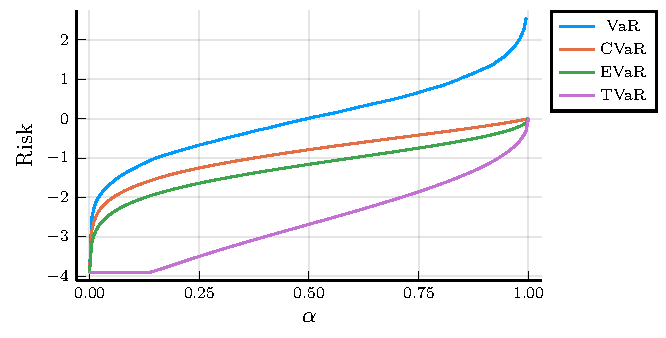
\includegraphics[width=0.5\linewidth]{figs/fast-risk/normal_comparison.pdf}
  \caption{Comparison of risk measure values for a normal distribution with mean $0$ and standard deviation $1$ as a function of the risk level $\alpha$.}
  \label{fig:comparison}
\end{figure}

An important property of TVaR is that it bounds EVaR~\cite{Ahmadi-Javid2012,Hau2023a,Su2025} from below, as we show next and illustrate in \cref{fig:comparison}.
\begin{proposition}
For each $\tilde{x} \in \mathbb{R}^n$, the risk measures above extended to $\alpha\in [0,1]$ satisfy that
\[
  \var{\alpha}{\tilde{x}}
  \; \ge\; 
  \cvar{\alpha}{\tilde{x}}
  \; \ge\; 
  \evar{\alpha}{\tilde{x}}
  \; \ge\; 
  \tvar{\alpha}{\tilde{x}}.
\]
\end{proposition}
\begin{proof}
 The inequality for VaR and CVaR is well known, and the inequality for CVaR and EVaR follows from \citep[proposition~3.2]{Ahmadi-Javid2012}. Recall that Pinsker's inequality~\citep[theorem~4.19]{boucheron2013concentration} shows for $\bm{p}, \bm{q}\in \Delta_n$ that $\| \bm{p} - \bm{q}\|_1 \le \sqrt{2 \kl(\bm{q} \| \bm{p})}$. Then we prove that TVaR lower-bounds EVaR as
\begin{align*}
\evaro_{\alpha}[\tilde{x}]
&=
\inf \left\{ \bm{q}\tr \bm{x} \mid \bm{q}\in \Delta_n, \kl(\bm{q} \| \bm{p}) \le \log \frac{1}{\alpha }, \bm{q} \ll \bm{p} \right\} \\
&\ge
\inf \left\{ \bm{q}\tr \bm{x} \mid \bm{q}\in \Delta_n, \| \bm{p} - \bm{q} \|_1 \le \sqrt{ 2 \log \frac{1}{\alpha }} , \bm{q} \ll \bm{p} \right\} \\
&=\inf \left\{ \bm{q}\tr \bm{x} \mid \bm{q}\in \Delta_n, \| \bm{p} - \bm{q} \|_1 \le \min \left\{  \sqrt{ 2 \log \frac{1}{\alpha }}, 2\right\}, \bm{q} \ll \bm{p}\right\}
= \tvaro_{\alpha }[\tilde{x}].
\end{align*}
Recall that $\| \bm{p} - \bm{q}\|_1 \le 2$.
\end{proof}

\section{Computing VaR in Linear Time} \label{sec:var-linear}

We now describe the QuickVaR algorithm, show that it computes VaR, and show that it runs in linear expected time. 

The standard VaR algorithm for a discrete random variable $\bm{x}\in \Real^n$ with distribution $\bm{p}\in \Delta_n$ and risk level $\alpha$ proceeds as follows~\citep[listing~6.25]{privault2026notes}. It sorts the entries of $\bm{x}$ to get a permutation $\sigma \colon 1{:}n \to 1{:}n$ such that $i \mapsto x_{\sigma(i)}$ is monotone. Then, it finds an index $i \in 1{:}n$ such that
\[
  \sum_{j = 1}^{i-1} p_{\sigma(j)}
  \; \le \;
  \alpha
  \; <\;
  \sum_{j = 1}^i p_{\sigma(j)}.
\]
The value $x_{\sigma(i)}$ is the optimal solution in~\eqref{eq:var-definition} by \cref{thm:quantile-in-finite-omega} below. The computational complexity of this algorithm is $\Omega(n \log  n)$ because its runtime is dominated by the need to sort the entries of $\bm{x}$. For the sake of completeness, \cref{alg:slow-quantile} in the appendix summarizes the standard greedy approach to computing VaR. 

\emph{QuickVaR}, described in \cref{alg:quick-quantile}, computes VaR in expected $O(n)$ time by avoiding the need to sort the elements of the input random variable $\bm{x}$. In particular, QuickVaR partially sorts the indices of $\bm{x}$, analogous to the quickselect algorithm~\cite{horowitz1998computer}. 

\Cref{alg:quick-quantile} is recursive and applies for a risk level $\alpha$ to a random variable $\bm{x}$ with a distribution $\bm{p}\in \Delta_n$ as follows. In addition, the input is $f$ (front) and $b$ (back), which delimit the indices of $\bm{x}$ it manipulates. The algorithm first picks a pivot element $v = x_j$ with $j$ chosen uniformly at random from $f{:}b$. The random pivot selection is essential to achieve an expected linear time complexity. Given a pivot, we use $\operatorname{partition}$ to partially sort the entries of $\bm{x}$ into three ranges, where $l$ and $g$ are the indices returned by $\operatorname{partition}$: $G_0 = f{:}(l-1)$, $G_1 = l{:}g$, and $G_2 = (g+1){:}b$. These three ranges satisfy $\bm{x}_{G_0} < v$, $\bm{x}_{G_1} = v$, $\bm{x}_{G_2} > v$. Then, the algorithm checks for the conditions of \cref{thm:quantile-in-finite-omega} to determine which of the three ranges contains the VaR value. Finally, if the VaR value is in range $G_0$ or $G_2$, the algorithm calls itself recursively with adjusted $f$, $b$, and $\alpha$.

The $\operatorname{partition}$ procedure in \cref{alg:quick-quantile} uses the Dutch national flag algorithm to partition the input array into the three groups. The algorithm runs in linear time, and the properties of its output are given in \cref{lem:hoare-partition}. For the sake of completeness, we provide the reader with the algorithm in \cref{alg:partition} in \cref{sec:stand-var-algor}. 

We present \cref{alg:quick-quantile} recursively to simplify its analysis. However, a loop-based, non-recursive implementation, such as \cref{alg:quickvar-nonrecursive} in \cref{sec:stand-var-algor}, typically performs better in imperative languages. 

\begin{algorithm}
  \caption{\texttt{QuickVaR}: Recursive VaR algorithm (when $f=1, b=n$)} \label{alg:quick-quantile}
  \Input{$\bm{x} \in \Real^n$, $\bm{p} \in \Delta_n$, $\alpha \in [0,1)$, $f, b \in 1{:}n$ such that $f \le  b$ and $\sum_{j=f}^b p_j > \alpha$}
  \Output{$\varo_{\alpha}[\tilde{x}]$}
  $v \gets x_{\operatorname{rand}(f{:}b)}$ \tcp*{Pivot}
  $l, g, \bm{x}', \bm{p}' \gets \operatorname{partition}(\bm{x}, \bm{p}, v, f, b)$
  \tcp*{~\cref{alg:partition}}
  \label{ln:t}
  $t \gets \sum_{j=f}^{l-1} p'_j$ \tcp*{$t = \P{\tilde{x} < v} - \sum_{i=1}^{f-1} p_i $}
  \label{ln:e}
  $e \gets \sum_{j=l}^{g} p'_j$  \tcp*{$e = \P{\tilde{x} = v}$}
  \label{ln:firstif}
  \If(\tcp*[f]{$\alpha + \sum_{i=1}^{f-1} p_i  < \P{\tilde{x} < v}$}){$\alpha < t$}{ 
    \KwRet{$\qvar(\bm{x}', \bm{p}', \alpha, f, l-1)$}
  }
  \label{ln:secondif}
  \ElseIf(\tcp*[f]{$\P{\tilde{x} \le v} \le \alpha + \sum_{i=1}^{f-1} p_i $}){$t + e \le \alpha$}{
    \KwRet{$\qvar(\bm{x}', \bm{p}', \alpha - t - e, g+1, b)$}
  }
  \label{ln:thirdif}
  \lElse{
    \KwRet{$v$}
  }
\end{algorithm}


The following theorem states the correctness of QuickVaR.
\begin{theorem} \label{thm:var-correct}
\Cref{alg:quick-quantile} executed with $f = 1$ and $b = n$ and $\alpha\in [0,1)$ returns $\varo_{\alpha}[ \tilde{x} ]$.
\end{theorem}

Before proving \cref{thm:var-correct}, we need to show several important lemmas. The following lemma, which holds only for discrete random variables, shows that the VaR value is a probability atom of the distribution of $\tilde{x}$ that satisfies \eqref{eq:var-property-prob}.
\begin{lemma}\label{thm:quantile-in-finite-omega}
Assuming $\alpha\in [0,1)$, there exists $\omega\in\Omega$ with $v := \var{\alpha }{\tilde{x}} = x_{\omega}$ and
\begin{equation} \label{eq:var-property-prob}
  \P{\tilde{x} < v} \le \alpha < \P{\tilde{x} \le v}. 
\end{equation}
\end{lemma}
\begin{proof}
First, we show that any $v$ that satisfies~\eqref{eq:var-property-prob} solves~\eqref{eq:var-definition} optimally. The implication $\P{\tilde{x} < v} \le \alpha \implies v \in \left\{ t \in \Real \mid  \P{ \tilde{x} < t } \le \alpha \right\}$ follows immediately. Second, we prove $\alpha < \P{ \tilde{x} \le v } \implies \forall t \in \left\{ t \in \Real \mid  \P{ \tilde{x} < t } \le \alpha \right\}, v \ge t$ by contradiction. Suppose that $\exists t \in \left\{ t \in \Real \mid  \P{ \tilde{x} < t } \le \alpha \right\}, v < t$. Then, by the monotonicity of the probability operator, we get a contradiction as
 \[
   \alpha
   < \P {  \tilde{x} \le v  }
   \le \P {  \tilde{x} < t  }
   \le \alpha.
 \]
Then, the existence of $x_{\omega} = v$ follows from \cref{lem:prob-lumpy} because~\eqref{eq:var-property-prob} implies that 
  \[
    \P{\tilde{x} =
      \var{\alpha }{\tilde{x}}} = \P{\tilde{x} \le \var{\alpha }{\tilde{x}}}  - \P{\tilde{x} < \var{\alpha }{\tilde{x}}} > \alpha - \alpha = 0.
  \]
Note that since $\Omega$ is finite and $\alpha<1$, the solution $v := \min\{x_\omega \mid \P{\tilde{x} \le x_\omega} > \alpha\}$ exists.
\end{proof}

The following lemma shows the recursive property of QuickVaR and is the main building block of \cref{thm:var-correct}.
\begin{lemma} \label{lem:quickvar-correct}
Suppose that the input conditions of \cref{alg:quick-quantile} hold and $\bm{x} \in \Real^n$ satisfies that
 \begin{equation} \label{eq:qvar-precondition}
  \max \bm{x}_{1{:}(f-1)} <  \min \bm{x}_{f{:}b},  \qquad
  \max \bm{x}_{f{:}b} < \min \bm{x}_{(b+1){:}n},
\end{equation} 
where $x_0 = -\infty$ and $x_{n+1} = +\infty$. Then \cref{alg:quick-quantile} returns $x_{\omega}, \omega\in f{:}b$ such that
\begin{equation} \label{eq:qvar-postcondition}
  \P{\tilde{x} < x_{\omega}}
  \quad \le \quad
  \alpha + \sum_{i=1}^{f-1} p_i 
  \quad < \quad \P{\tilde{x} \le x_{\omega}}.
\end{equation}
\end{lemma}
\begin{proof}
From~\eqref{eq:qvar-precondition} and \cref{lem:hoare-partition}, $t$ and $e$ on lines~\ref{ln:t} and \ref{ln:e} satisfy that
\begin{equation} \label{eq:te-equivalence}
  t = \P{\tilde{x} < v} - \sum_{i=1}^{f-1} p_i , \qquad e = \P{\tilde{x} = v}.
\end{equation}
We proceed by induction on $k = b - f$. \emph{Base case}: $k = 0$. Since $b = f$, we have that $v = x_b$ and $l = g = b$, $t = 0$, $e = p_b$, and $\alpha  \ge t$. The input condition implies that $t + e = p_b > \alpha$. Because $t \le \alpha < p_b$, the algorithm returns $v$ on line~\ref{ln:thirdif} that satisfies
\[
 \P{\tilde{x} < v} \le \alpha + \sum_{i=1}^{f-1} p_i < \P{\tilde{x} \le v}. 
\]
Above, the first inequality follows from $v = x_f$ and $0 \le \alpha$. The second inequality follows from the algorithm's input condition.  

\emph{Inductive step}. Suppose that $k>0$ and that the result holds for each $k' < k$. Then:

(i) If $\alpha < t$, the algorithm executes the first if statement on line~\ref{ln:firstif}. Because $0 \le \alpha  < t$, the recursive call satisfies the required input conditions: $f \le l-1$ and $\sum_{j=f}^{l-1} p_j = t > \alpha$. The recursive call also satisfies~\eqref{eq:qvar-precondition} by \cref{lem:hoare-partition}, and we can conclude that~\eqref{eq:qvar-postcondition} follows from the inductive hypothesis because $l-1 - f \le b-1 -f \le k-1 < k$. 

(ii) If $t + e \le \alpha$, the algorithm executes the second if statement on line~\ref{ln:secondif}. We show that the input conditions for the recursive call are met. Because $t + e = \sum_{j = f}^g p_j \le \alpha < \sum_{j=f}^b p_j$  (the second inequality is the input condition), it must be that $g < b$ and therefore $g+1 \le b$. Also, by the algorithm's input condition and algebraic manipulation, we get that
\[
 \sum_{j=g+1}^b p_j = \sum_{j=f}^b p_j - t - e > \alpha - t - e,
\]
and the input conditions hold.  Because~\eqref{eq:qvar-precondition} follows from \cref{lem:hoare-partition} and $b - g - 1 < b-f \le  k$, the inductive hypothesis implies that there exists $x_{\omega}$ such that
\[
  \P{\tilde{x} < x_{\omega}}
  \quad \le \quad
  (\alpha - t - e) + \P{\tilde{x} \le v}
  \quad < \quad \P{\tilde{x} \le x_{\omega}}. 
\]
Then,~\eqref{eq:qvar-postcondition} follows by algebraic manipulation after substituting $t,e$ from~\eqref{eq:te-equivalence}.

(iii) If $t \le \alpha < t + e$, the algorithm executes the else statement on line~\ref{ln:thirdif}, and the inequality~\eqref{eq:qvar-postcondition} holds by substituting $t,e$ from~\eqref{eq:te-equivalence}.
\end{proof}

We are now ready to prove the correctness of QuickVaR.
\begin{proof}[Proof of \cref{thm:var-correct}]
With $f = 1$ and $b = n$, the condition in~\eqref{eq:qvar-precondition} holds vacuously, and the input condition $\sum_{j=1}^n p_j = 1 > \alpha$ holds since $\alpha\in [0,1)$. Therefore, \cref{lem:quickvar-correct} shows that QuickVaR returns $x_{\omega}$ that satisfies
  \[
  \P{\tilde{x} < x_{\omega}}
  \quad \le \quad
  \alpha 
  \quad < \quad \P{\tilde{x} \le x_{\omega}}, 
\]
which satisfies~\eqref{eq:var-property-prob} and, therefore, it equals the VaR value by 
  \cref{thm:quantile-in-finite-omega}. 
\end{proof}

With the correctness of \cref{alg:quick-quantile} established in \cref{thm:var-correct}, we now show its computational complexity. 
\begin{theorem} \label{prop:time-complexity}
\Cref{alg:quick-quantile} runs in expected $O(n)$ time.
\end{theorem}
\begin{proof}
The proof is analogous to the standard quickselect algorithm, as in theorem~3.3 in \citet{horowitz1998computer}, except that we need to keep track of the risk level $\alpha$. Fix some $n \in \mathbb{N}$, $\bm{x}$, and $\bm{p}$, and we study the algorithm's properties. Let $T\colon 1{:}n \to [0,\infty]$ be the \emph{expected} runtime of \cref{alg:quick-quantile} such that $T(k)$ is the expected runtime when executed with $k := b - f + 1$ for the worst-case of the other parameters. Note that $T(k)$ is monotone.  To simplify the notation, we assume without loss of generality in the remainder of the proof that $f = 1$ and $b = k$. Then, let
\[
  l := \left| \left\{ i \in 1{:}k \mid  x_i < \varo_{\alpha}[\tilde{x}]\right\}   \right|.
\]
Note that by the assumption $\sum_{j = f}^b p_j > \alpha$, we have that $k \ge 1$ and $\varo_{\alpha}[\tilde{x}] \le \max_{i\in f{:}b} x_i$. Therefore, $l \in 0{:}(k-1)$. The algorithm terminates in constant time when $k = 1$, and we upper-bound the runtime for the worst-case choice of $l$ for $k > 1$ as
\begin{align}
\nonumber
  T(k)
  &\le d\cdot k + \max_{l\in 0{:}(k-1)} \frac{1}{k} \sum_{i=0}^{k-1} \left(   T(i) \cdot 1_{l < i} + T(k - i - 1) \cdot 1_{l > i}  \right) \\
\nonumber
  &= d\cdot k + \max_{l\in 0{:}(k-1)} \frac{1}{k}  \left(  \sum_{i=l+1}^{k-1} T(i)  + \sum_{i=0}^{l-1} T(k - i - 1)   \right) \\
\label{eq:quickvar-complexity}
  &= d\cdot k + \max_{l\in 0{:}(k-1)} \frac{1}{k}  \left(  \sum_{i=l+1}^{k-1} T(i)  + \sum_{i=k-l}^{k-1} T(i)   \right),
\end{align}
where $d\cdot k$ is the local runtime of the algorithm for some $d > 0$ and $T(i)$ and $T(k - i - 1)$ are the average runtimes of the recursive calls. The average over $i$ corresponds to the uniformly random selection of the pivot index with $i = \left| \left\{ j \in 1{:}k \mid x_j < v \right\} \right|$ in the first line of the inequality. When multiple elements are equal to the pivot value, the inequality follows from the monotonicity of $T$. The last two equalities follow by algebraic manipulation. Then, an argument identical to~\citet[theorem 3.3]{horowitz1998computer}, since~\eqref{eq:quickvar-complexity} is the same as equation~(3.8) in~\citet{horowitz1998computer}, shows that \(T(k)\le 4\cdot d\cdot k\) for all \(k\ge 1\).
\end{proof}
 
\begin{remark} \label{rem:weighted-median}
  An attentive reader may notice that QuickVaR resembles the algorithm for computing the weighted median~\cite[section~17.1]{Korte2012}. However, the weighted median algorithm does not, in general, compute VaR. Define the \emph{quantile} $\quant_{\alpha},\alpha \in (0,1)$ for $\tilde{x}$ as the closed set
\[
 \quant_{\alpha}[\tilde{x}] := \left\{ z\in \Real \mid  \P{ \tilde{x} \le z } \ge \alpha, \P{ \tilde{x} \ge z } \ge 1-\alpha  \right\},
\]
with bounds $\quant^+_{\alpha}[\tilde{x}] := \max \quant_{\alpha}[\tilde{x}]$ and $\quant^-_{\alpha}[\tilde{x}] := \min \quant_{\alpha}[\tilde{x}]$. One can readily show that $\varo_{\alpha }[\tilde{x}] = \quant^+_{\alpha}[\tilde{x}]$. Although the precise definition of a weighted median varies, it is typically a value in $\quant_{\frac{1}{2}}[\tilde{x}]$. Because $\quant^+_{\alpha}[\tilde{x}] \neq \quant^{-}_{\alpha}[\tilde{x}]$, in general, VaR also does not equal the median. A careful analysis shows that the weighted median algorithm in~\citet[section~17]{Korte2012} computes $\quant^-_{\frac{1}{2}}[\tilde{x}]$, which does not equal $\varo_{\frac{1}{2}}[\tilde{x}]$ in general.
\end{remark}

\section{Computing \texorpdfstring{$\varphi$}{phi}-divergence Risk Measures in Linear Time} \label{sec:phi-divergence}

In this section, we describe and analyze QuickDivergence, a new linear-time framework for computing a class of $\varphi$-divergence risk measures, including CVaR and TVaR. QuickDivergence treats risk evaluation as a linear optimization over a polymatroid. Standard polymatroid optimization algorithms must sort their input, which requires $\Omega(n \log  n)$ runtime. We identify a structural condition of polymatroid risk measures that allows us to avoid sorting and instead use the linear-time QuickVaR algorithm described in \cref{sec:var-linear}.

The remainder of the section is organized as follows. \Cref{sec:quickdivergence} describes a general linear-time algorithm suitable for $\varphi$-divergence risk measures that satisfy an EWS property~(\cref{asm:submodular-function}). Then \cref{sec:cvar-tvar-are} shows that both CVaR and TVaR satisfy the EWS property and can be computed in linear time. Note that we use a fixed distribution $\bm{p} \in \Delta_n$ and omit it in the notation when it is obvious from the context.

\subsection{QuickDivergence} \label{sec:quickdivergence}
We first recall the definition of a submodular function~\cite[section~2.1]{Korte2012} and a polymatroid~\cite[definition~14.9]{Korte2012}.
\begin{definition} \label{def:polymatroid}
A function $f \colon 2^{1{:}n} \to \Real_{\ge 0}$ is \emph{submodular} if
\[ 
  f(\mathcal{A}) + f(\mathcal{B})
  \; \geq\;
  f(\mathcal{A} \cup \mathcal{B}) + f(\mathcal{A} \cap \mathcal{B}),
  \quad
  \forall \mathcal{A}, \mathcal{B} \subseteq 1{:}n.
\]
For a submodular \emph{capacity} function $f \colon 2^{1{:}n} \to \Real_{\ge 0}$, a \emph{polymatroid} $\mathcal{Q}_f$ is a polytope defined as
  \[
    \mathcal{Q}_f
    \;:=\;
    \left\{ \bm{q} \in \Real_{\ge 0}^n  \mid   \bm{1}\tr_{\mathcal{U}} \bm{q} \leq f(\mathcal{U}), \, \forall \,  \mathcal{U} \subseteq 1{:}n \right\},
\]
and a \emph{normalized polymatroid} is $\widehat{\mathcal{Q}}_f := \mathcal{Q}_f \cap \Delta_n $.
\end{definition}


Polymatroids are useful in optimization because any coherent, comonotonic monetary risk measure can be formulated as linear optimization over a polymatroid~\cite[theorems~4.88 and~4.94]{Follmer2016}. Recall that a risk measure $\rho$ is \emph{coherent} if it is concave and positively homogeneous.  A risk measure $\rho$ is \emph{comonotonic} (additive) if for any comonotone $\tilde{x}, \tilde{y}$: $\rho[ \tilde{x} + \tilde{y} ] = \rho[ \tilde{x} ] + \rho[ \tilde{y} ]$, where the random variables $\tilde{x}, \tilde{y} \in \Real^n$ are \emph{comonotone} if $(\tilde{x}(i) - \tilde{x}(j))(\tilde{y}(i) - \tilde{y}(j)) \ge 0$ for each $i,j\in 1{:}n$.

\begin{proposition} \label{prop:coherent-polymatroid}
A monetary risk measure $\rho\colon \Delta_n \times  \Real^n \to \Real$ is a coherent comonotonic risk measure if and only if
\begin{equation}\label{eq:comonotonic-optimization}
  \rho[\tilde{x}] = \min_{\bm{q}\in \widehat{\mathcal{Q}}_c} \bm{q}\tr  \bm{x},
  \qquad
  \text{where}
  \qquad
  c(\mathcal{A}) := -\rho[ -\tilde{1}_{\mathcal{A}} ], \quad \forall  \mathcal{A} \subseteq 1{:}n,
\end{equation}
where $\tilde{1}_{\mathcal{A}}$ is the indicator random variable of $\mathcal{A}$. Moreover, if the risk measure is law-invariant, then there exists $g\colon \Real \to \Real$ such that $c(\mathcal{A}) = g(\bm{1}\tr \bm{p}_{\mathcal{A}})$ for each $\mathcal{A} \subseteq 1{:}n$.
\end{proposition}

\Cref{prop:coherent-polymatroid} follows  from theorems~4.88 and~4.94 in~\citet{Follmer2016}.

The standard solution to the polymatroid optimization problem in~\eqref{eq:comonotonic-optimization} is to use a greedy algorithm, such as \cref{alg:greedy-polymatroid}. This algorithm adapts the standard polymatroid optimization, such as \citet[section~14.2]{Korte2012}, to the normalized polymatroid $\widehat{\mathcal{Q}}_f$. See \cref{prop:standard-polymatroid-works} for the proof of correctness. Note that the greedy approach in \cref{alg:greedy-polymatroid} requires sorting and, therefore, runs in $\Omega(n \log  n)$ time.

\begin{algorithm}
    \caption{Linear minimization over normalized polymatroids.} \label{alg:greedy-polymatroid}
    \Input{submodular monotone function $f \colon  2^{1{:}n} \to \Real_{\ge 0}$, and an objective $\bm{x}\in \Real^n$}
    \Output{$\hat{\bm{q}} \in \argmin_{\bm{q}\in \widehat{\mathcal{Q}}_f} \bm{x}\tr \bm{q}$}
    Use sort to get
    $\sigma \colon 1{:}n \to 1{:}n$ such that
    $i > j \implies x_{\sigma(i)} \ge  x_{\sigma(j)}, \; \forall i, j \in 1{:}n$\;
     \For{$k\in 1{:}n$}{
       $\hat{q}_{\sigma(k)} \gets f\left(\sigma(1{:}k)\right) - f\left(\sigma(1{:}(k-1))\right) $
    }
    \Return{$\hat{\bm{q}}$}
\end{algorithm}

We now define a special class of submodular functions, called EWS, that makes sorting unnecessary when optimizing a linear function over a polymatroid.
\begin{definition} \label{asm:submodular-function}
A function $f\colon 2^{1{:}n} \to \Real_{\ge 0}$ is $\ews(\bm{\mu} ,m, \kappa)$, or \emph{Element-Wise-Separable}, for $\kappa \in \Real_{\ge 0}$,  $m\in \Real_{>0}$, such that $\kappa \le 1$, $\kappa + m \ge 1$, and $\bm{\mu}\in \Delta_n$ if $f(\mathcal{A}) = g(\bm{1}\tr \bm{\mu}_{\mathcal{A}})$ for all $\mathcal{A}\subseteq 1{:}n$ and
\begin{equation} \label{eq:def-g}
    g(x) :=
    \begin{cases}        
    \min \{\kappa + m  \cdot x, 1\} &\text{if } x > 0, \\
    0 &\text{otherwise}.
    \end{cases}
\end{equation}
\end{definition}

EWS functions satisfy the properties necessary to define a polymatroid as we show next.
\begin{proposition}
An EWS function $f\colon 2^{\Omega} \to  \Real_{\ge 0}$ is submodular, monotone, and satisfies that $f(\emptyset) = 0$, and $f(\Omega) = 1$.
\end{proposition}
\begin{proof} 
To show that $f$ is submodular, it is sufficient, from \cref{lem:submodular-concave}, to show that $g$ is concave and monotone on $[0,1]$. The function $g$ is concave on $(0, 1]$ because it is the minimum of two affine functions~\cite{boyd2004convex}. To extend concavity to $[0,1]$ observe that $g(0) = 0$ and for each $\lambda \in (0,1]$ and $b \in ( 0, 1]$ we have
\begin{align*}
  (1 - \lambda)g(0) + \lambda \cdot g(b)
  = \lambda \cdot g(b)
  = \min\left\{\lambda  \cdot \kappa + m\cdot \lambda\cdot b, \lambda\right\} 
  \leq \min \left\{ \kappa + m \cdot \lambda \cdot b, 1 \right\}
  % = g(\lambda \cdot  b)
  = g\left( (1 - \lambda)\cdot 0 + \lambda\cdot b\right).
\end{align*}
Because the inequality also holds for $\lambda = 0$, $g$ is concave on $[0,1]$ by the definition. The monotonicity, non-negativity and the boundary value conditions for $f$ follow by algebraic manipulation from the assumptions on $\kappa$ and
$m$.
\end{proof}

\begin{algorithm}
  \caption{\texttt{QuickDivergence}: Linear minimization over EWS polymatroids.} \label{alg:maximum-weight-independent}
  \Input{$\bm{x} \in \Real^n$, $\bm{p} \in \Delta_n$, $\ews(\bm{p}, m, \kappa)$ function $f \colon 2^{1{:}n} \to \Real_{\ge 0}$}
  \Output{$\bm{q}\opt \in \argmin_{\bm{q} \in \widehat{\mathcal{Q}}_f} \bm{x}\tr\bm{q}$}
  Choose $k_{\min} \in \argmin_{i \in  1{:}n} x_i \; \operatorname{s.\,t.}\; p_i > 0$; break ties to choose the smallest $i$ \tcp{Analogous to $\ess\inf$}
    $v \gets
    \begin{cases}
      \operatorname{QuickVaR}(\bm{x}, \bm{p}, (1 - \kappa)/m, 1, n), &\text{ if } (1-\kappa) / m < 1, \\
      \infty, &\text{ otherwise}
    \end{cases}
     $\;
  $\mathcal{K}_{< v} \gets \{ i \in  1{:}n \mid x_i < v \}$ ;~
  $\mathcal{K}_{= v} \gets \{ i \in 1{:}n \mid x_i = v \}$ \;
  $l \gets |\mathcal{K}_{< v} \cup \{ k_{\min} \} |$\;
  $\theta_l \gets  1 - \min \left\{ \kappa + m\cdot \bm{1}\tr \bm{p}_{\mathcal{K}_{<v} \cup \{k_{\min}\} }, 1 \right\}$ \;
  \For{$i \in 1{:}n$}{
    \lIf{$i = k_{\min}$}{$q\opt_i \gets \min \left\{  m\cdot p_i + \kappa, 1\right\}$ }
   \lElseIf{$i \in \mathcal{K}_{< v}$} {$q\opt_i \gets m \cdot p_i$}
   \lElseIf{$i \in \mathcal{K}_{=v}$} {$q\opt_i \gets \min \left\{  \theta_l, \, m \cdot p_i \right\} $;~ $\theta_{l+1}\gets \theta_l - q\opt_i;~ l \gets l+1$}
   \lElse{$q\opt_i \gets 0$}
  }
  \Return{$\bm{q}\opt$}
 \end{algorithm}

\Cref{alg:maximum-weight-independent} describes \emph{QuickDivergence}, an algorithm for polymatroid optimization. QuickDivergence differs from the standard linear polymatroid algorithm in \cref{alg:greedy-polymatroid} in that it does not require sorting the input vector. Instead, the algorithm uses QuickVaR to partially sort the input vector.

The following theorem states the correctness and runtime of \cref{alg:maximum-weight-independent}. 
\begin{theorem} \label{thm:quickdivergence-correct}
  \Cref{alg:maximum-weight-independent} solves~\eqref{eq:comonotonic-optimization} in expected $O(n)$ runtime.
\end{theorem}
\begin{proof}
To prove the correctness of \cref{alg:maximum-weight-independent}, we show that it returns $\bm{q}\opt$ that equals $\hat{\bm{q}}$ returned by the standard \cref{alg:greedy-polymatroid}.  Suppose that \cref{alg:greedy-polymatroid} chooses a permutation $\sigma\colon  1{:}n \to 1{:}n$ such that $i \le j \Rightarrow x_{\sigma(i)} \le x_{\sigma(j)}$ and $x_{\sigma(i)} = x_{\sigma(j)} \wedge i < j \Rightarrow \sigma(i) < \sigma(j)$ for each $i,j\in 1{:}n$. In other words, the permutation $\sigma$ needs to be generated by a stable sort algorithm except that it satisfies that $\sigma^{-1}(k_{\min}) < \sigma^{-1}(i)$ for each $i \neq k_{\min}$ such that $x_i = x_{k_{\min}}$. That is, $k_{\min}$ is sorted to be first among elements of the same value. We emphasize that the stability assumption is only needed for our proof technique; the actual implementation does not require it. Also, the standard \cref{alg:greedy-polymatroid} works with any valid sort order. 

We now prove that $q\opt_i = \hat{q}_i$ for each $i\in 1{:}n$ by separately analyzing the following four cases.

\emph{(i)} Suppose that $i = k_{\min}$. Because $p_i > 0$ from the construction of $k_{\min}$ then
\[
  q\opt_i = \min \left\{   m\cdot p_i + \kappa, 1 \right\} = g(p_i) =  g(p_i) - g(0) = f(\{ i \} \cup \mathcal{J}) - f(\mathcal{J})  = \hat{q}_i,
\]
where $\mathcal{J} := \{ j \in 1{:}n \mid \sigma^{-1}(j) < \sigma^{-1}(i) \}$ and $\bm{1}_{\mathcal{J}}\tr \bm{p} = 0$ by the construction of $k_{\min}$.

\emph{(ii)} Suppose that $i \in \mathcal{K}_{<v} \wedge i \neq k_{\min}$. First, assume that $x_i \ge x_{k_{\min}}$. From \cref{thm:quantile-in-finite-omega}, we get for each $\mathcal{O} \subseteq \mathcal{K}_{<v}$ that
\begin{equation} \label{eq:lt-v-prob}
 \bm{1}\tr \bm{p}_{\mathcal{O}} \le \P{\tilde{x} < v} \le \frac{1-\kappa}{m},
\end{equation}
and, hence, from~\eqref{eq:def-g}:
\(  f(\mathcal{O}) = g\left(\bm{1}\tr \bm{p}_{\mathcal{O}}\right) = \kappa + m \cdot \bm{1}\tr \bm{p}_{\mathcal{O}},
  \text{ when }
  \bm{1}\tr \bm{p}_{\mathcal{O}} > 0.
\) 
Let $k := \sigma^{-1}(i)$ and note that $ \sigma(1{:}k) \subseteq \mathcal{K}_{< v} $ because if $l \in 1{:}k$, then $x_{\sigma(l)} \le x_{\sigma(k)} = x_i < v$ and $\sigma(l) \in \mathcal{K}_{< v}$. Then, since $i \neq k_{\min}$:
\[
 \hat{q}_i = \hat{q}_{\sigma(k)} = f(\sigma(1{:}k)) - f(\sigma(1{:}(k-1)))
= m \cdot \bm{1}\tr \bm{p}_{\sigma(1{:}k) \setminus \sigma(1{:}(k-1)) } = m\cdot p_{\sigma(k)} = m\cdot p_i = q\opt_i. 
\]
The third equality follows from $i \neq k_{\min}$ and $p_{k_{\min}} \neq  0$. Second, if $x_i < x_{k_{\min}}$  then $\hat{q}_i = 0 = m p_i = q\opt_i$ by construction. 

\emph{(iii)} Suppose that $i \in \mathcal{K}_{=v} \wedge i \neq k_{\min}$. Here, we use the assumption that $\sigma$ is a stable sort and prove the claim by induction on $l \in |\mathcal{K}_{<v} \cup \{k_{\min}\}|, \dots, |\mathcal{K}_{<v}\cup \{k_{\min}\}| + |\mathcal{K}_{=v} \setminus \{ k_{\min}\}| - 1$ showing that
\begin{align}
 \label{eq:theta-equality-1}
  \theta_l &= 1 - f(\sigma(1{:}l)),  \\
  \label{eq:theta-equality-2}
    \hat{q}_{\sigma(l+1)} &= q\opt_{\sigma(l+1)}.
\end{align}
To prove the base case, suppose that $l = |\mathcal{K}_{<v} \cup \{k_{\min}\}|$. The equality in~\eqref{eq:theta-equality-1} holds by algebraic manipulation from~\eqref{eq:def-g} since $\mathcal{K}_{<v} \cup \{ k_{\min} \} = \sigma(1{:}l)$. The equality in~\eqref{eq:theta-equality-2} follows from~\eqref{eq:def-g} and~\eqref{eq:lt-v-prob}. First, assume that $\theta_l > 0$; then
\begin{equation} \label{eq:q-q-eq}
  \begin{aligned}
\hat{q}_{i} = \hat{q}_{\sigma(l+1)}  
  &= f ( \sigma(1{:}(l+1) )) - f ( \sigma(1{:}l) ) \\
  &= \min \left\{  1,\; \kappa + m \cdot \bm{1}\tr \bm{p}_{\sigma(1{:}(l+1))} \right\} - \kappa - m \cdot \bm{1}\tr \bm{p}_{\sigma(1{:}l)} \\
  &= \min \left\{1  - \kappa - m \cdot \bm{1}\tr \bm{p}_{\sigma(1{:}l)}, \; m \cdot p_{\sigma(l+1)}\right\} \\
  &= \min \{ \theta_l, m \cdot p_i \} = q_i\opt.
  \end{aligned}
\end{equation}
When $\theta_l = 0$, we get by algebraic manipulation that $\hat{q}_i = 0 = q\opt_i$.

To prove the inductive case, suppose that~\eqref{eq:theta-equality-1} and~\eqref{eq:theta-equality-2} hold for $l$, and we prove it for $l+1$. The equality in~\eqref{eq:theta-equality-1} can be derived from~\eqref{eq:theta-equality-2} and the construction in \cref{alg:greedy-polymatroid} as
\begin{align*}
  \theta_{l+1}
  = \theta_l - q\opt_{\sigma(l+1)} 
    = \theta_l - \hat{q}_{\sigma(l+1)}
    = 1 - f(\sigma(1{:}l)) - \left(  f(\sigma(1{:}(l+1))) - f(\sigma(1{:}l)) \right) 
  = 1 - f(\sigma(1{:}(l+1))).
\end{align*}
The equality in~\eqref{eq:theta-equality-2} follows analogously to~\eqref{eq:q-q-eq} if $\theta_{l+1} > 0$:
\begin{equation} \label{eq:q-q-eq-2}
  \begin{aligned}
\hat{q}_{i} = \hat{q}_{\sigma(l+2)}
  &= f ( \sigma(1{:}(l+2) )) - f(\sigma(1{:}(l+1))) \\
  &= \min \left\{  1,\; \kappa + m \cdot \bm{1}\tr \bm{p}_{\sigma(1{:}(l+2))} \right\} - (1-\theta_{l+1}) \\
  &= \min \left\{\theta_{l+1}, \;\kappa + m \cdot \bm{1}\tr \bm{p}_{\sigma(1{:}(l+2))} - f(\sigma(1{:}(l+1))) \right\} \\
  &= \min \left\{\theta_{l+1}, \; m \cdot p_{\sigma(l+2)}  \right\} 
  = q_i\opt.
  \end{aligned}
\end{equation}
If $\theta_{l+1} = 0$, we get by algebraic manipulation that $\hat{q}_i = 0 = q\opt_i$.


\emph{(iv)} Suppose that $i \in \mathcal{K}_{>v} := \{ j \in 1{:}n \mid x_j > v \}$ and let $k = \sigma^{-1}(i)$. Then, using~\eqref{eq:var-property-prob} we have that:
\begin{align*}
  1
  \ge f(\sigma(1{:}k))
  \ge f(\sigma(1{:}(k-1))) 
  \ge \min \{\kappa + m \cdot \bm{1}\tr \bm{p}_{\sigma(1{:}(k-1))}, 1\}
  \ge 1,
\end{align*}
since $\bm{1}\tr\bm{p}_{\sigma(1{:}(k-1))} > \frac{1-\kappa}{m}$ from \cref{thm:quantile-in-finite-omega} and the construction of $v$ in \cref{alg:maximum-weight-independent}. Then
\[
  \hat{q}_i = \hat{q}_{\sigma(k)}
  =  f(\sigma(1{:}k)) - f(\sigma(1{:}(k-1)))
  = 0 = q\opt_i.
\]

\end{proof}

\subsection{Solving CVaR and TVaR in Linear Time} \label{sec:cvar-tvar-are}

We show that CVaR and TVaR are two examples of $\varphi$-divergence risk measures that can be formulated as linear optimization over a polymatroid with an EWS capacity function and, therefore, can be solved in linear time. To formulate the CVaR polymatroid optimization, we define the capacity function $f_{\alpha}^{\cvaro}\colon 2^{\Omega } \to \Real$  for each $\mathcal{O} \subseteq \Omega$ and $\alpha \in [0,1]$ as
\begin{equation} \label{eq:f-cvar}
  f_{\alpha}^{\cvaro}(\mathcal{O})
    \;:=\;
      \begin{cases}
        \min\left\{\frac{1}{\alpha} \cdot \P{\mathcal{O}}, 1\right\} & \text{if } \alpha \in (0,1], \\
        0 & \text{if } \alpha = 0 \wedge \P{\mathcal{O}} = 0,  \\
        1 & \text{if } \alpha = 0 \wedge \P{\mathcal{O}} > 0. 
      \end{cases} 
\end{equation}
The capacity function $f_{\alpha }^{\cvaro}$ for CVaR defined in~\eqref{eq:f-cvar} is well known, but is usually restricted to $\alpha\in (0,1)$~\cite{acerbi2002spectral}. The following proposition states its correctness; its proof is in the appendix.
\begin{proposition} \label{prop:cvar-ews-correct}
For each $\alpha\in [0,1]$, $\tilde{x} \colon \Omega \to \Real$, and $\bm{p} \in \Delta_n$: 
\begin{equation} \label{eq:cvar-correct}
  \cvar{\alpha }{\tilde{x} }
  \;=\;
  \min_{\bm{q} \in \widehat{\mathcal{Q}}_{f_{\alpha }^{\cvaro}}} \bm{x}\tr \bm{q}.
\end{equation}
Moreover, $f^{\cvaro}_{\alpha }$ is $\ews(\bm{p}, 1/\alpha, 0)$ when $\alpha > 0$, and $\ews(\bm{p}, 1, 1)$ when $\alpha = 0$.
\end{proposition}

To compute TVaR, we define the capacity function $f_{\alpha}^{\tvaro}\colon 2^{\Omega } \to \Real$  for each $\mathcal{O} \subseteq \Omega$ and $\alpha \in [0,1]$ as
\begin{equation}\label{eq:f-tvar}
  f^{\tvaro}_{\alpha}(\mathcal{O})
    \; :=\; 
      \begin{cases}
        \min\left\{\P{\mathcal{O}} + \min \left\{ \sqrt{\frac{1}{2} \log \frac{1}{\alpha}}, 1\right\}, 1\right\} &\text{if } \alpha \in (0,1] \wedge \P{\mathcal{O}} > 0, \\
        0 & \text{if } \P{\mathcal{O}} = 0, \\
        1 & \text{if } \alpha = 0 \wedge \P{\mathcal{O}} > 0.
      \end{cases}
\end{equation}

TVaR has been proposed in the context of $\varphi$-divergence risk measures~\cite{Kruse2021} as well as in the context of robust stochastic programming~\cite{Shapiro2017}. TVaR is also very closely related to the $L_1$ ball used in robust Markov decision processes~\cite{Ho2021,Ho2022}. However, we are not aware of prior work that defines or uses the capacity function in~\eqref{eq:f-tvar}. The following proposition (see the appendix for the proof) shows that this function can be used to correctly formulate the TVaR evaluation using an EWS function. 
\begin{proposition} \label{prop:tvar-ews-correct}
For each $\alpha\in [0,1]$, $\tilde{x} \colon \Omega \to \Real$, and $\bm{p} \in \Delta_n$: 
\begin{equation} \label{eq:tvar-correct}
  \tvar{\alpha}{\tilde{x} } = \min_{\bm{q}\in \widehat{\mathcal{Q}}_{f_{\alpha}^{\tvaro}}} \bm{x}\tr \bm{q}.
\end{equation}
Moreover, $f^{\tvaro}_{\alpha }$ is $\ews(\bm{p}, 1, \min \left\{   \sqrt{\frac{1}{2}  \log \frac{1}{\alpha}}, 1 \right\})$  when $\alpha > 0$, and $\ews(\bm{p}, 1, 1)$ when $\alpha = 0$.
\end{proposition}

Combining \cref{thm:quickdivergence-correct} with \cref{prop:cvar-ews-correct,prop:tvar-ews-correct} yields the main result of this section: CVaR and TVaR can be computed in expected linear time without sorting.
\begin{corollary} \label{cor:cvar-tvar-linear}
For each $\alpha\in [0,1]$, $\tilde{x} \colon \Omega \to \Real$, and $\bm{p} \in \Delta_n$, let $\bm{q}\opt_{\cvaro}$ and $\bm{q}\opt_{\tvaro}$ be the vectors returned by \cref{alg:maximum-weight-independent} with the capacity functions $f^{\cvaro}_{\alpha}$ and $f^{\tvaro}_{\alpha}$, respectively. Then
\[
  \cvar{\alpha}{\tilde{x}} = \bm{x}\tr \bm{q}\opt_{\cvaro}
  \qquad \text{and} \qquad
  \tvar{\alpha}{\tilde{x}} = \bm{x}\tr \bm{q}\opt_{\tvaro},
\]
and both values can be computed in expected $O(n)$ time.
\end{corollary}
\begin{proof}
Because $f^{\cvaro}_{\alpha}$ and $f^{\tvaro}_{\alpha}$ are EWS with the stated parameters by \cref{prop:cvar-ews-correct,prop:tvar-ews-correct}, they can be optimized with \cref{alg:maximum-weight-independent}. \Cref{thm:quickdivergence-correct} then shows that $\bm{q}\opt_{\cvaro}$ and $\bm{q}\opt_{\tvaro}$ minimize $\bm{x}\tr\bm{q}$ over $\widehat{\mathcal{Q}}_{f^{\cvaro}_{\alpha}}$ and $\widehat{\mathcal{Q}}_{f^{\tvaro}_{\alpha}}$, respectively, in expected $O(n)$ time. The equalities follow from~\eqref{eq:cvar-correct} and~\eqref{eq:tvar-correct}, and computing the inner product $\bm{x}\tr\bm{q}\opt$ adds only $O(n)$ time.
\end{proof}

\section{Experiments}\label{sec:experiments}

\begin{figure}
  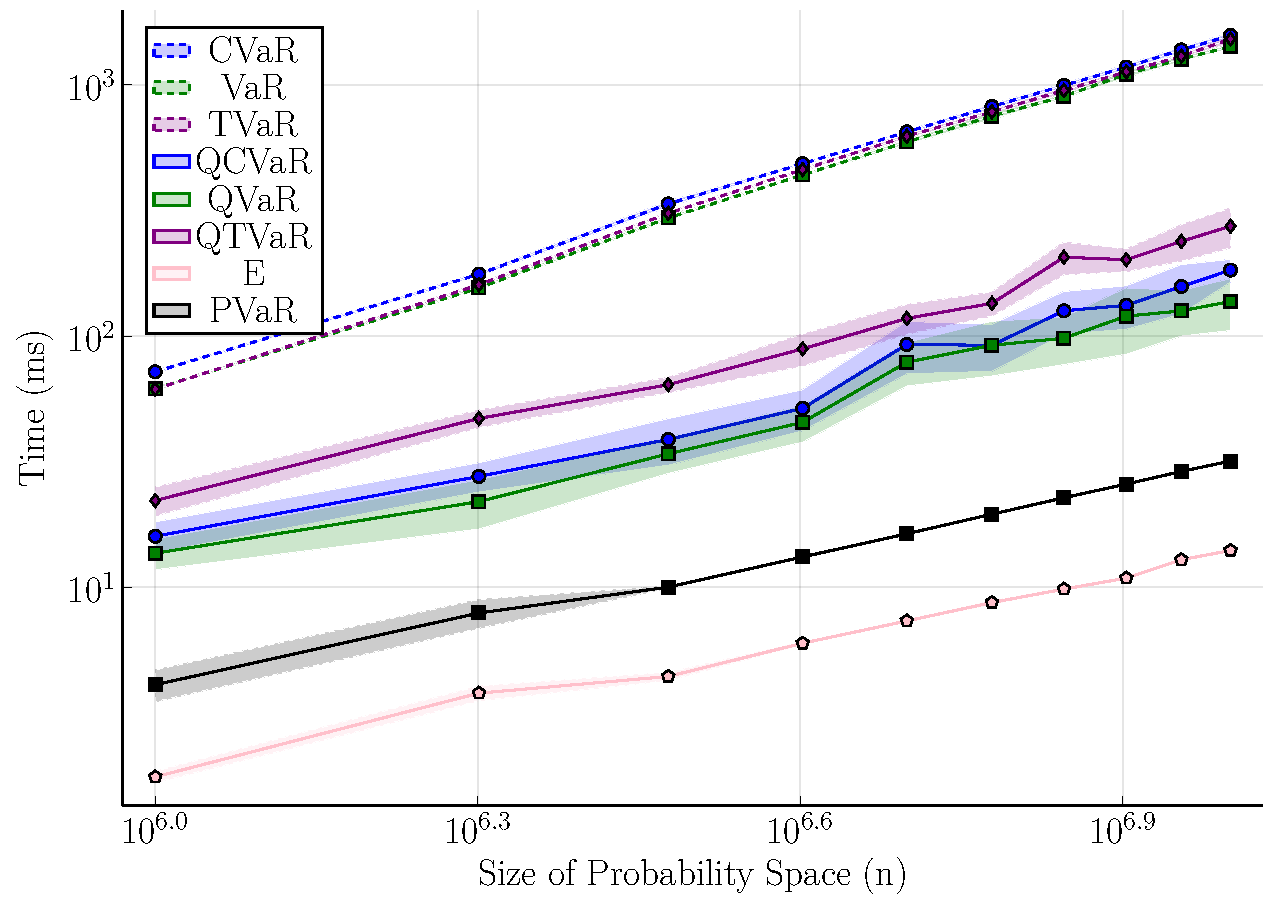
\includegraphics[width=0.48\textwidth]{figs/fast-risk/benchmark_random_uniform.pdf}
  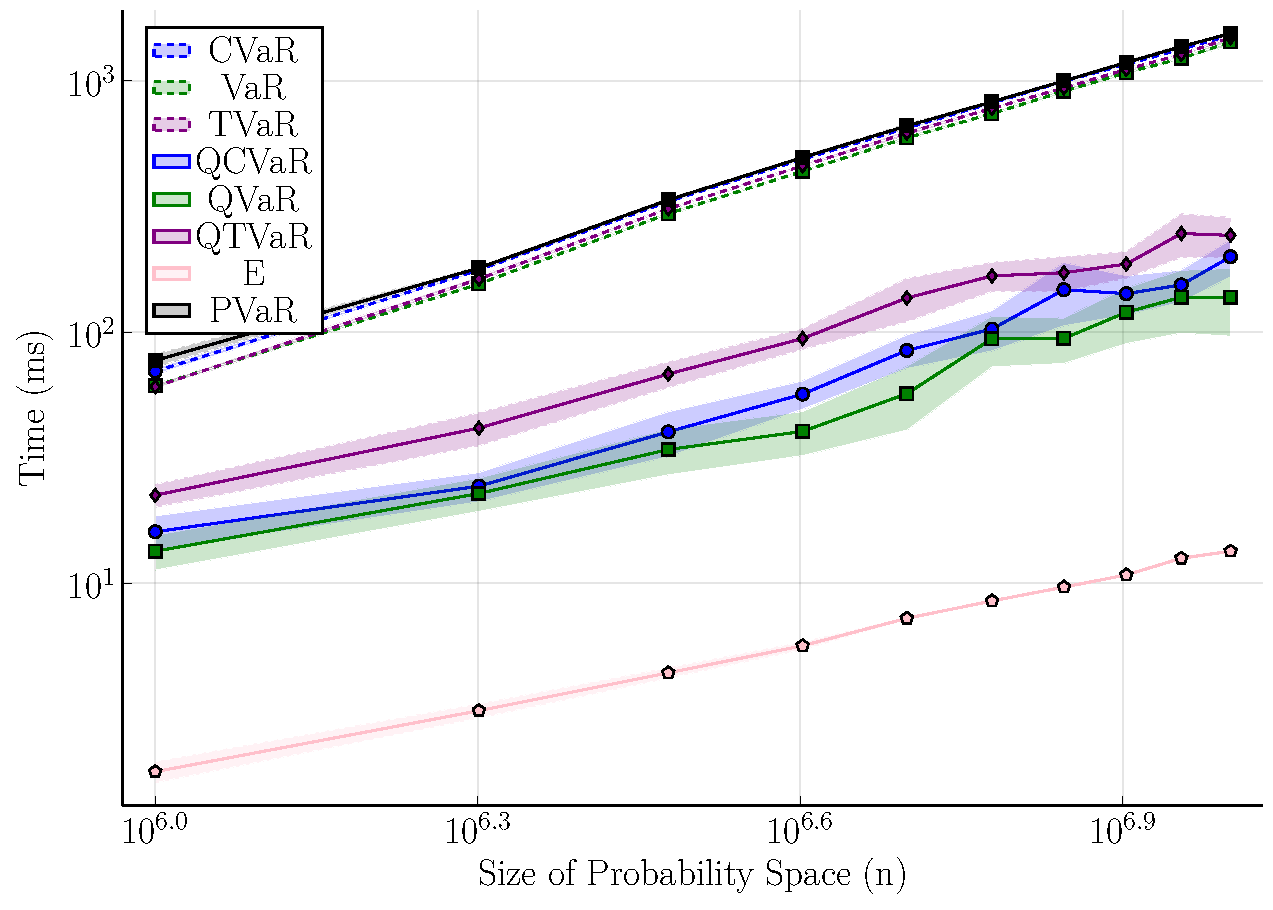
\includegraphics[width=0.48\textwidth]{figs/fast-risk/benchmark_random_sparse.pdf}
  \caption{Algorithms' runtime  for samples from a \emph{uniform} random variable (left) and a \emph{sparse} random variable (right). Shaded regions denote $95\%$ confidence bands over $10$ independent runs.}
  \label{fig:benchmarks}
\end{figure}


We evaluate the proposed algorithms empirically to confirm that their theoretical performance guarantees translate into faster practical runtimes. We compare each linear-time algorithm against its standard sorting-based counterpart. Throughout this section, we prefix the name of our linear-time implementation with a ``Q'' to distinguish it from the sorting-based baseline, giving QVaR, QCVaR, and QTVaR. We also report the runtime of computing the standard expectation $\mathbb{E}$ as a baseline.

Our implementation, along with the code and data needed to reproduce all results, is available at \url{https://github.com/marekpetrik/paper_lineartime_risk}, and the implementation of the risk measures is available at \url{https://github.com/RiskAverseRL/RiskMeasures.jl}. We ran all experiments on an AMD Ryzen Threadripper 3970X with 32~cores and 64~threads at $4.5$\,GHz and $256$\,GB of RAM using Julia~1.13.1. To reduce noise in the timing measurements, we disable the Julia garbage collector during each run. In addition to standard baselines, we also compare the runtime of QVaR with a PVaR algorithm that uses Julia's \texttt{partialsort!} function directly to avoid sorting. With uniform weights $\bm{p}$, PVaR computes a $k \in \Nats$ analytically such that the $k$-th largest element of $\bm{x}$ equals VaR. Then, it uses \texttt{partialsort!} to find this element. When $\bm{p}$ are not uniform, PVaR computes the minimum range $k{:}l$ of possible indices of $\bm{x}$ that equals VaR. PVaR then sorts the $k{:}l$ largest elements of $\bm{x}$ and searches them for the actual VaR value. The range $k{:}l$ is computed from $\min_{i\in 1{:}n} p_i$ and $\max_{i\in 1{:}n} p_i$.

We begin with synthetic data drawn from a uniform distribution with $n$ samples, varying $n$ from $10^6$ to $10^7$. For each value of $n$ we run every algorithm $10$ times on independently generated samples and report the mean runtime. \Cref{fig:benchmarks} shows the results on a log-log scale for random variables with uniform (left) and sparsely-supported (right) distributions. We fix the risk level to $\alpha = 0.95$, though the results are similar for other levels except the degenerate cases $\alpha = 0$ and $\alpha = 1$. The shaded regions denote $95\%$ confidence bands over the $10$ runs; the bands are tight because the measured runtimes vary little between runs. 

The results confirm that the quick algorithms are substantially faster than their sorting-based counterparts, with the gap widening as $n$ grows. This behavior matches the theoretical analysis of \cref{sec:var-linear,sec:phi-divergence}: the sorting-based methods require $O(n \log n)$ operations, whereas our algorithms run in $O(n)$ expected time, so the logarithmic factor separating them grows with the size of the probability space. The acceleration is most consequential for VaR and CVaR, which are the most widely used risk measures in the applications discussed in \cref{sec:intro} and are frequently evaluated on large random variables.

As expected, PVaR outperforms QVaR for a uniform distribution since the partial sort need not manipulate the constant list of probabilities $\bm{p}$. When the probabilities are constant, PVaR is preferable to QVaR and can also serve as a basis for implementing QTVaR and QCVaR. However, when the probability weights $\bm{p}$ are not uniform, the partial sort algorithm must sort most of the random variable's values. As a result, PVaR's runtime on a non-uniform distribution is similar to that of sort-based algorithms. 

\begin{table}
\centering
\caption{Algorithms' runtime (ms) in the stock market scenario.}
\label{tab:stock}
\begin{tabular}{lrr}
\toprule
Method & Mean & St. D. \\
\midrule 
VaR & 0.37 & 0.00 \\ 
QVaR & 0.13 & 0.02 \\
\midrule 
CVaR & 0.39 & 0.00 \\ 
QCVaR & 0.22 & 0.03 \\ 
\midrule 
TVaR & 0.40 & 0.01 \\ 
QTVaR & 0.25 & 0.05 \\ 
\midrule 
$\mathbb{E}$ & 0.01 & 0.00 \\
\bottomrule
\end{tabular}
\end{table}

\begin{table}
\centering
\caption{Algorithms' mean runtime (ms) on small sparse domains.}
\begin{tabular}{rrrrrrrr}
\toprule
n & $\mathbb{E}$ & VaR & QVaR & CVaR & QCVaR & TVaR & QTVaR \\
\midrule
1000 & 0.00 & 0.03 & 0.01 & 0.03 & 0.02 & 0.03 & 0.02\\
2000 & 0.00 & 0.06 & 0.02 & 0.06 & 0.03 & 0.06 & 0.04\\
3000 & 0.01 & 0.09 & 0.04 & 0.10 & 0.05 & 0.10 & 0.07\\
4000 & 0.00 & 0.13 & 0.04 & 0.14 & 0.06 & 0.13 & 0.08\\
5000 & 0.01 & 0.16 & 0.05 & 0.17 & 0.10 & 0.18 & 0.10\\
6000 & 0.00 & 0.20 & 0.08 & 0.21 & 0.10 & 0.21 & 0.11\\
7000 & 0.00 & 0.23 & 0.08 & 0.25 & 0.12 & 0.24 & 0.13\\
8000 & 0.00 & 0.27 & 0.09 & 0.28 & 0.13 & 0.28 & 0.15\\
9000 & 0.01 & 0.30 & 0.09 & 0.32 & 0.12 & 0.31 & 0.17\\
10000 & 0.01 & 0.33 & 0.11 & 0.35 & 0.16 & 0.35 & 0.19\\
\bottomrule
\end{tabular}
\label{tab:small_results}
\end{table}

To confirm the speedups persist beyond large synthetic inputs, we repeat the comparison on two more realistic settings. The first one is a stock market scenario, in which the random variable models the returns of a financial portfolio. \Cref{tab:stock} reports the mean runtime and standard deviation of each method. The second setting consists of small-scale problems, where the asymptotic advantage is least pronounced but can be practically important when the risk measures must be computed repeatedly. \Cref{tab:small_results} reports the mean runtime on sparse random variables over probability spaces of size $n$ ranging from $1000$ to $10\,000$, using the same protocol as above but with $50$ trials per configuration in place of $10$. Even at these sizes, the quick algorithms outperform their sorting-based counterparts for every method and every value of $n$, confirming that the linear-time algorithms deliver consistent improvements across the full range of input sizes without incurring any penalty on small inputs.

Finally, we evaluate the algorithms in a small experiment using risk-averse value iteration with a nested risk measure~\cite{Behzadian2021a,Hau2023a,Hau2023}. This example shows how the methods would be used in an actual reinforcement learning problem. Risk-averse value iteration evaluates the risk measure multiple times during every iteration. The domain we use is the inventory management problem~\cite{Hau2023} with 50--400 states and with half as many actions as states. We use the nested risk measure objective~\cite{Hau2023} which applies the risk measure iteratively in every iteration with fixed $\alpha=0.95$. As before we verified that changing $\alpha$ does not drastically affect runtime, except in degenerate cases. \Cref{tab:rl-inventory} shows the results. The results indicate that even small risk-averse reinforcement learning problems can benefit from no-sort algorithms when using risk-averse value iteration.

\begin{table}
  \centering
  \caption{Algorithms' runtime (ms) when used as a part of a reinforcement learning benchmark optimizing a risk-averse objective in an inventory management domain.}
  \label{tab:rl-inventory}
\begin{tabular}{rrrrrrrr}
\toprule
n & $\mathbb{E}$ & VaR & QVaR & CVaR & QCVaR & TVaR & QTVaR \\
\midrule
50 & 38.74 & 51.49 & 34.70 & 58.86 & 43.18 & 64.15 & 62.10\\
100 & 533.07 & 675.98 & 551.23 & 751.08 & 632.28 & 774.17 & 762.19\\
200 & 2080.17 & 3041.41 & 2134.01 & 3610.40 & 2737.83 & 3821.01 & 3669.45\\
400 & 5645.05 & 10914.77 & 5929.39 & 15436.73 & 8643.82 & 17063.76 & 16656.26\\
\bottomrule
\end{tabular}
\end{table}
 

\section{Conclusion}

We propose and analyze new algorithms for computing several common risk measures, including VaR, CVaR, and TVaR, in $O(n)$ expected time, where $n$ is the size of the probability space. This compares favorably with the $O(n \log n)$ time required by sorting-based methods.  This speedup is significant because risk measures are frequently evaluated on large random variables in applications such as robotics, finance, and energy system planning. An important direction for future work is to develop fast algorithms for other risk measures, such as EVaR and expectiles.

\subsubsection*{Acknowledgments}

This work was supported, in part, by NSF grants 2144601 and 2218063. The authors would also like to thank Wheeler Ruml for helpful discussions.

% !TEX root = ../main.tex
\chapter{Conclusion}\label{ch:conclusion}

\todo{summary and future work}


% UNH: references single-spaced, with a blank line between entries
\begingroup
\singlespacing
\setlength{\bibsep}{\baselineskip}
\bibliographystyle{abbrvnat}
\bibliography{thesis}
\endgroup

\appendix
% !TEX root = ../main.tex
\chapter{Supplementary Materials for \texorpdfstring{Chapter~\ref{ch:roil}}{Chapter 3}}\label{app:roil}

% ---- ported from the appendix of github.com/GersiD/ChebyshevROIL paper/RIRL_NHT.tex ----
\section{Proofs} % of \cref{sec:basic-formulation}}
\label{sec:appendix_proofs}
\begin{lemma}\label{prop:convexity_of_Upsilon}
The set $\Upsilon$ is non-empty, convex, compact, and polyhedral.
\end{lemma}
\begin{proof}
The set is non-empty because $u_{\mathrm{e}}\opt  \in \Upsilon$. It is convex and polyhedral from its construction and is compact because it is bounded ($1\tr u \le  \nicefrac{1}{1-\gamma}$) and closed.  
% Since $\mathcal{U}$ is the set of feasible solutions to the dual LP formulation~\cite[Eq.~(6.9.2)]{Puterman1994} it is well known to be polyhedral and convex. To show that the set $\mathcal{U}$ is compact, we need to show that it is bounded. This is true since, $u \in \mathcal{U}$ satisfies $u \ge 0$ by construction, and it is easy to verify that $1\tr u = \frac{1}{1-\gamma}$. Then, the set $\Upsilon$ is an intersection of half-spaces with $\mathcal{U}$ a closed convex set. Any union of closed half-spaces is convex and closed~\cite[eq.~(2.2.1)]{boyd_convex_optimization}.
\end{proof}

\lemmaOccupancyExistance*
\begin{proof}
We prove the two implications individually.

\emph{Case 1:} Prove $u \in \Upsilon   \quad \Rightarrow \quad  \exists
        \pi \in \Pi_{\mathrm{R}}(\mathcal{D}), \, u = u^{\pi}$,

Given a $u \in \Upsilon$, we have that $u^{\pi_{u}} = u$ since $u\in \mathcal{U}$ and $p_0 > 0$. Recall that $p_0 >0 $ guarantees that
\[
  \sum_{a\in \mathcal{A}} u(s,a) \ge  p_0 > 0, \quad \forall s\in \mathcal{S}.
\]
We now show that $\pi^u \in \Pi_{\mathrm{R}}(\mathcal{D})$. The constraint on $u\in \Upsilon$ combined with $u > 0$ implies that for each $(\cdot , s, \cdot ) \in \mathcal{D}$:
\begin{alignat*}{2}
  && \sum_{a\in \mathcal{A} : a \neq \pi_{\mathrm{e}}(s)} u(s,a) &\;=\; 0, \\
    \ArrowBetweenLines[\Downarrow]
  && u(s,a) &\; =\; 0, \qquad \forall a\in \mathcal{A}, a \neq  \pi_{\mathrm{e}}(s) \\
    \ArrowBetweenLines[\Downarrow]
  && \pi^u(s,a) &\;=\; 0,  \qquad \forall a\in \mathcal{A}, a \neq \pi_{\mathrm{e}}(s).
\end{alignat*}
Therefore $\pi^u\in \Pi_{\mathrm{R}}(\mathcal{D})$, which proves the implication. 

\emph{Case 2:} Prove $\pi \in \Pi_{\mathrm{R}}(\mathcal{D}) \quad \Rightarrow \quad  u_{\pi} \in
        \Upsilon $

This follows because
\[
 c\tr u^{\pi} = \sum_{s\in \mathcal{S}} \sum_{a\in \mathcal{A}} c(s,a) u(s,a) = 0, 
\]
since $c(s,a) > 0 \Rightarrow \pi(s,a) = 0 \Rightarrow u(s,a) = 0$.
% Given that $\pi \in \Pi_{\mathrm{R}}(\mathcal{D})$, $\pi(a|s) = 1$ for all $(s,a) \in \mathcal{D}$. Therefore, for observed states $s$, $u(s,a) = 0$ for all $a \not= \pi_{\mathrm{e}}(s)$
% since $u(s,a) = \pi(a|s)\sum_{a'}{u_{\pi}(s,a')}$. Then we see that indeed for the $c$ as defined in case 1, $u\tr c = 0$.
\end{proof}

\section{Experimental Results Revisited}
\label{sec:experimental_results_revisited}
\begin{figure}
	\centering
	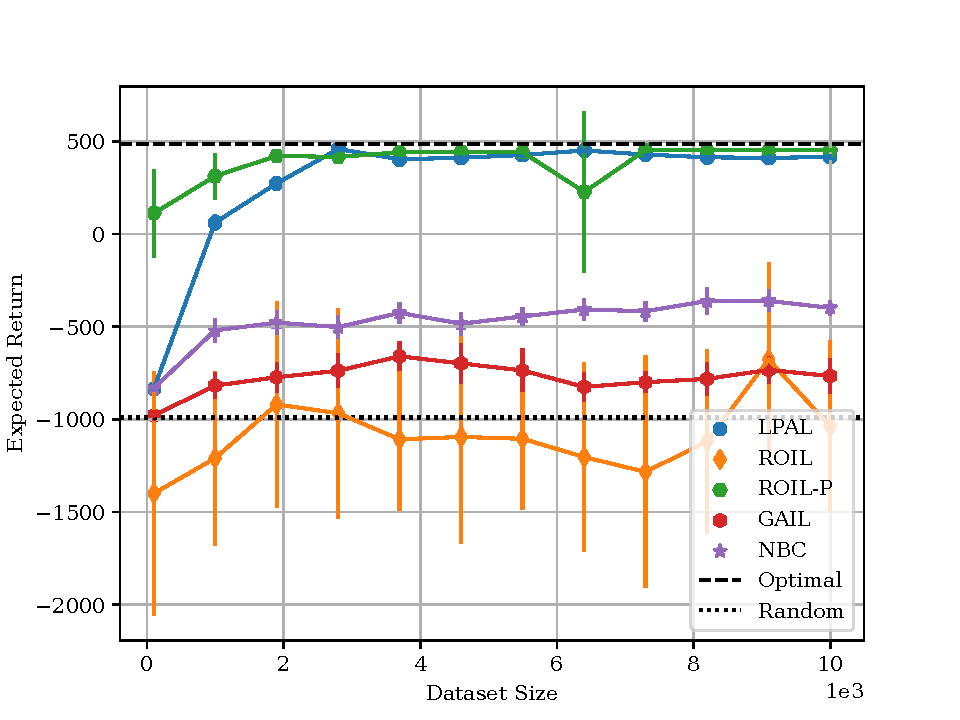
\includegraphics[width=0.45\textwidth]{figs/roil/40x40_driving_on_policy_returns.pdf}
	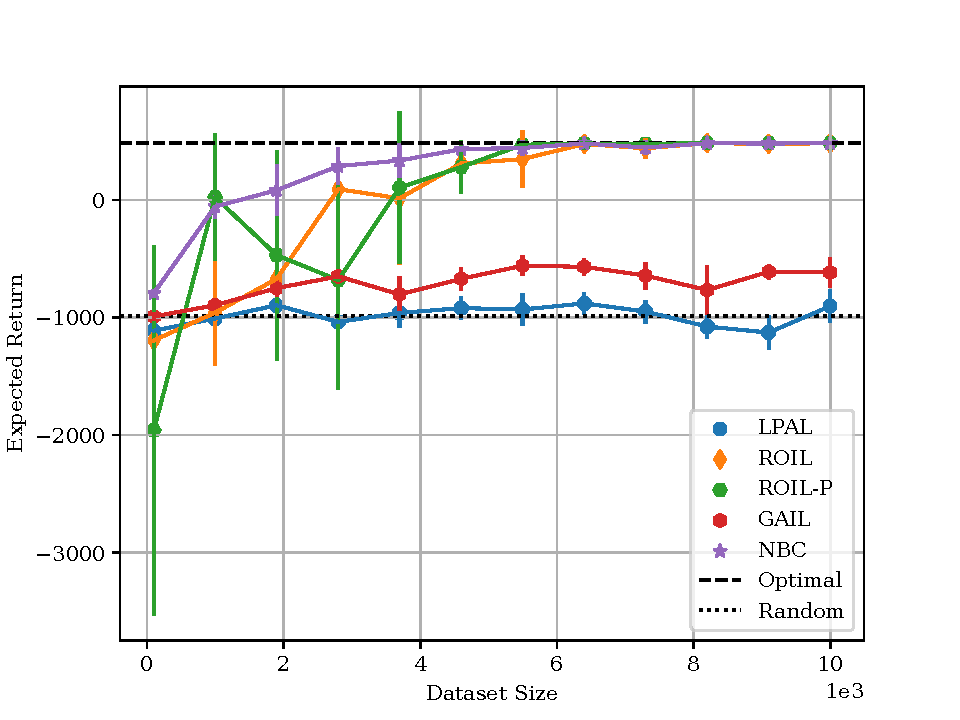
\includegraphics[width=0.45\textwidth]{figs/roil/40x40_driving_off_policy_returns.pdf}
	\caption{On (left) and off (right) policy 40x40 driving sim returns.}
	\label{fig:driving}
\end{figure}

\begin{figure}
	\centering
	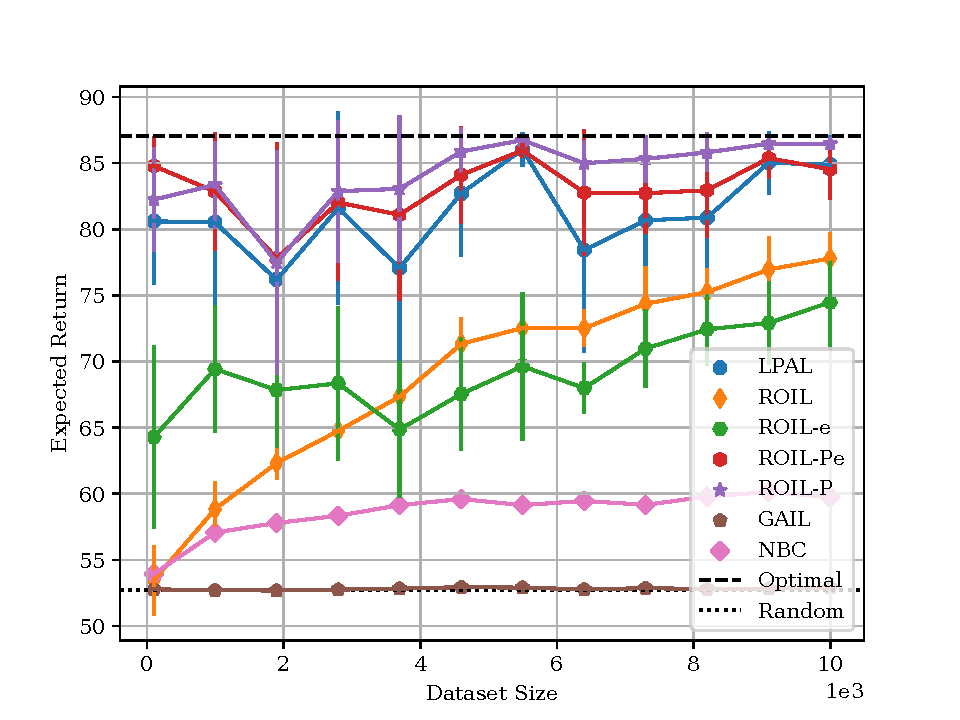
\includegraphics[width=0.45\textwidth]{figs/roil/40x40_gridworld_on_policy_all_returns.pdf}
	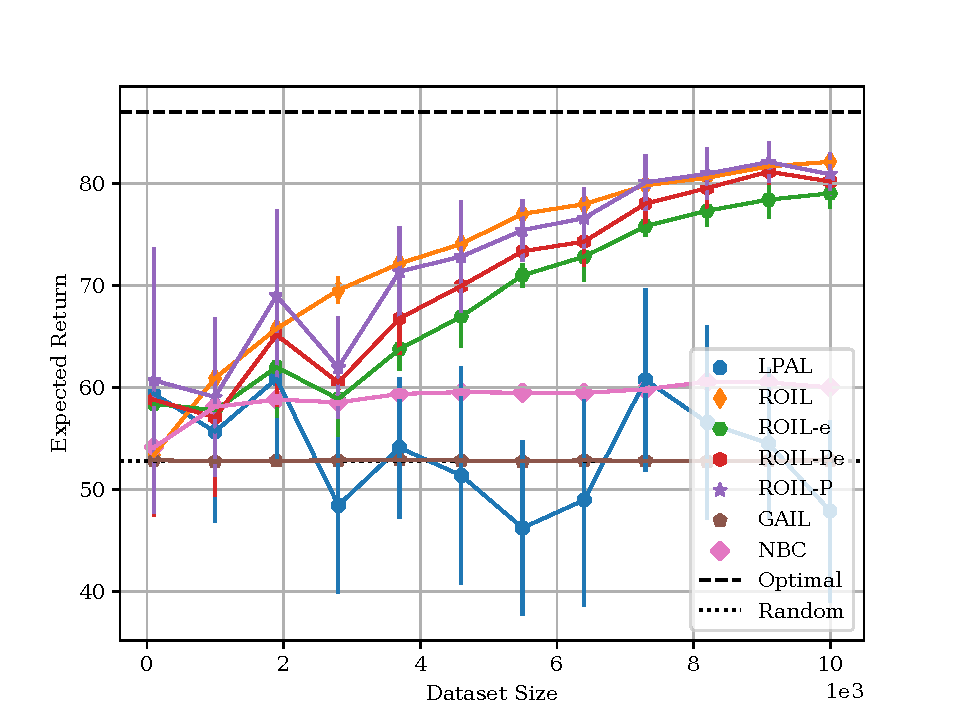
\includegraphics[width=0.45\textwidth]{figs/roil/40x40_gridworld_off_policy_all_returns.pdf}
	\caption{On (left) and off (right) policy 40x40 gridworld returns with more methods from \cref{sec:optimization-formulation}}
	\label{fig:more_methods_gridworld}
\end{figure}

\begin{figure}
	\centering
	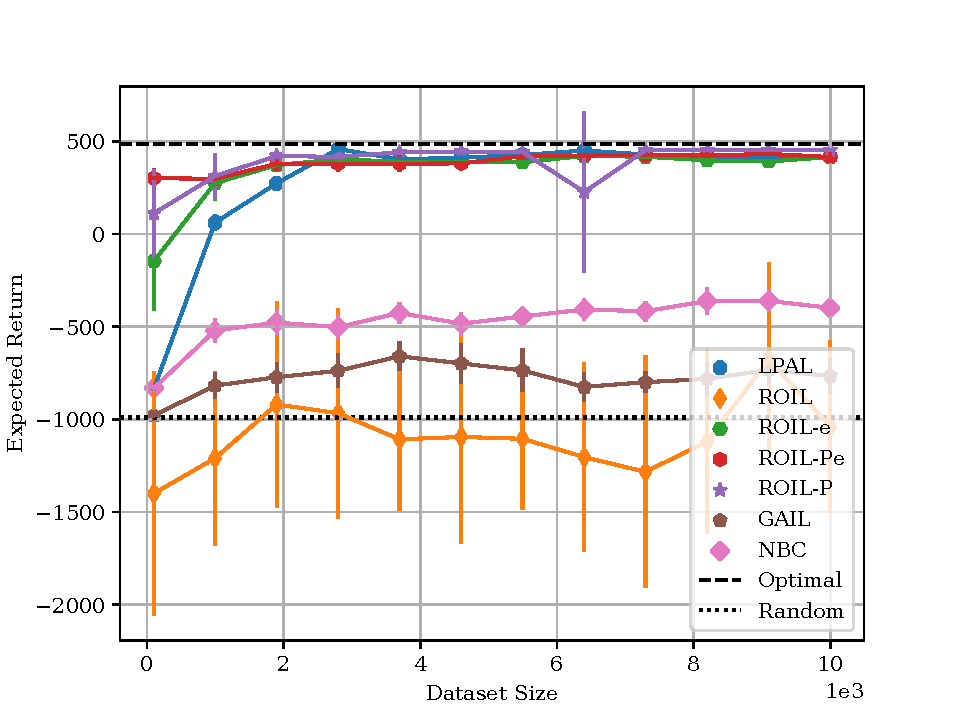
\includegraphics[width=0.45\textwidth]{figs/roil/40x40_driving_on_policy_all_returns.pdf}
	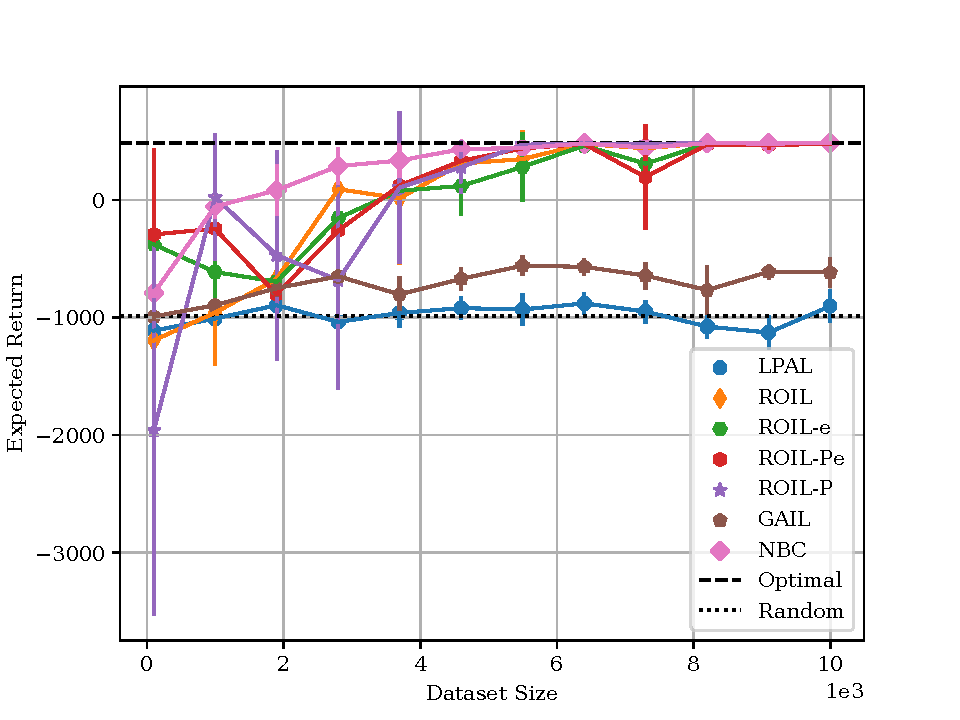
\includegraphics[width=0.45\textwidth]{figs/roil/40x40_driving_off_policy_all_returns.pdf}
	\caption{On (left) and off (right) policy 40x40 driving sim returns with more methods from \cref{sec:optimization-formulation}}
	\label{fig:more_methods_driving}
\end{figure}

We focus on describing the grid world environment; the driving environment is implemented similarly. The states of a grid world are integers from 0 to $N\times N$ where $N$ is the number of rows in the grid world, we assume we have square grid worlds where the number of columns and rows are the same. The actions an actor can take are up, down, left, and right. And the reward for a particular $(s,a)$ tuple is dictated by some reward vector $r \in \Real^{SA} = \Phi\tr w$ for some $w \in \mathcal{W}$. To solve all methods that rely on an LP, such as all ROIL variants described here, we rely on Gurobi~\cite{gurobi}. The feature vector for the grid world environment was the color of the current cell which was randomized for each seed, out of 4 total colors. For the driving simulator, there were also 4 features, current row, current column, whether the actor crashed in the current state, or whether the actor went off-road. \gersi{When constructing $D_e$ for off-policy experiments $\pi_e$ decides the actions for each state, however the state transitions came from a uniformly random policy $\pi_b$. More precisely $D_e = (s_t, \pi_e(s_t))_{t=0}^{D}$ where $s_{t+1} \sim P(s_t, \pi_b(s_t))$ and $s_0 \sim p_0$.}

\subsection{ROIL Variants}
\label{sec:roil_variants_appendix}
We focus on ROIL and ROIL-P. ROIL uses the linear constraint on $\mathcal{U}$ resulting in an outer minimization over $\Upsilon$ instead of $\mathcal{U}$ in \eqref{eq:extreme-points-reformulated} with the same inner maximization. ROIL-P uses pruning which is a technique to reduce the number of inner maximizations needed in the final minimization in \eqref{eq:extreme-points-reformulated}, we use $\hat{u}_e$ to prune away extreme points (or sampled points in cases where $\mathcal{W}$ leads to non-enumerable extreme points) where $\hat{u}_e\tr $ ext$(\mathcal{W}) \leq \tau$. 

For convenience, let $\psi \in \Real^d = \max_{v \in \Upsilon} v\tr\Phi w \;\; \forall w \in$ ext$(\mathcal{W})$ where $d$ is the number of inner maximizations you wish to solve, whether that be all extreme points of the L infinity norm ball or some sub-sample of a different norm ball. ROIL-P chooses $\tau$ to be the 90\% quantile of $\psi$. While it may seem ignorant to ignore some of these extreme points, it is a helpful heuristic that can help calibrate our pessimism as described in \cref{sec:optimization-formulation}. This extension as well as many others is what we find new and exciting about ROIL, however, we have too few pages to describe all such tweaks. For those interested, in \cref{fig:driving,fig:grid-40} we use $100$ samples from the $\Real_{1+}$ for ROIL-P.

We also implemented ROIL-e and ROIL-Pe which optimize over $\hat{\Upsilon}_\epsilon$ as in \cref{sec:incorp-addit-constr}, this led to comparable on policy performance to LPAL and ROIL-P while maintaining stable gains in expected return with new state action pairs off policy as seen in \cref{fig:more_methods_gridworld,fig:more_methods_driving}. However, due to how cluttered the graphs got, we decided to leave those as an extension and show off the two methods that were most representative of our formulation as a whole, putting the choice of robustness into the user's hands.

\subsection{GAIL}

While the performance of most methods seems about on par with what one would expect it may seem that our implementation of GAIL~\cite{Ho2016}
has some bugs. We assure the reader and refer the reader to our code \textcolor{red}{REDACTED} that we did indeed implement GAIL correctly and it does converge in smaller domains when $\mathcal{D}$ is on policy as the expectation in Algorithm 1 of~\cite{Ho2016} relies on $\hat{u}_{\mathrm{e}}$ being close to $u_{\mathrm{e}}\opt$. Due to computation constraints, and to be fair to the other methods we compared with, we had to limit the computation time per method. GAIL, being based on policy gradient methods, is rather sample inefficient concerning environment interactions~\cite[Section 7]{Ho2016} thus it incurs extra computation collecting on policy samples from $\pi_\theta$. We would also like to note that GAIL must bootstrap itself with a new random policy parameter $\theta$ each run as the other methods we tested against it also did not get to keep any information from previous runs.
% \roilLp*
% \begin{proof}
%   The result follows from the discussion in \cref{sec:basic-formulation} and by the epigraph formulation of~\eqref{eq:extreme-points-reformulated}.
    % Recall the definition of $\Phi \in \Real^{SA \times K}$ given some arbitrary ordering on $(s,a)$ pairs.
    % \begin{center}
    
    % 	\[\*\Phi\tr \;=\; \begin{bmatrix}
    % 			- & \phi_1\tr & - \\
    % 			- & \phi_2\tr & - \\
    % 			- & \vdots    & - \\
    % 			- & \phi_K\tr & -
    % 		\end{bmatrix}\]
    
    % 	Where $\phi_n = [\phi_n(s,a)\;\;\forall s,a \in S \times A]$ represents the n'th feature evaluated on each $(s,a)$ pair.
    % \end{center}
    
    % We apply a technique called Chebyshev Approximation~\cite{boyd_convex_optimization}(6.1) to equation~\eqref{eq:extreme_points_of_the_IRL_Formulation}.
    % This step can also be seen as writing~\eqref{eq:extreme_points_of_the_IRL_Formulation} in epigraph form.
    
    % \begin{equation}
    % 	\begin{mprog}
    % 		\minimize{u \in \mathcal{U}, \sigma \in \Real} \sigma
    % 		\stc \max_{v \in \Upsilon} |(v - u)\tr \Phi_i| \leq \sigma
    % 		\cs i \in 1 \dots k
    % 	\end{mprog}
    % \end{equation}
    
    % After expanding the absolute value is equivalent to.
    
    % \begin{equation}
    % 	\begin{mprog}
    % 		\minimize{u \in \mathcal{U}, \sigma \in \Real} \sigma
    % 		\stc \max_{v \in \Upsilon} (v - u)\tr \Phi_i \leq \sigma
    % 		\cs \max_{v \in \Upsilon} -(v - u)\tr \Phi_i \leq \sigma
    % 		\cs i \in 1 \dots k
    % 	\end{mprog}
    % \end{equation}
    
    % In order to make the above problem more easily solvable, let us take the dual of the first inner maximization problem.
    
    % \begin{equation}
    % 	\begin{mprog}
    % 		\maximize{v \in \Upsilon} (v - u)\tr \Phi_i
    % 		\cs i \in 1\dots k
    % 	\end{mprog}
    % \end{equation}
    
    % Notice in order to get this into an LP form we need to take the convex set $\Upsilon$ and construct a linear constraint which encapsulates what it means for an element $v \in \Real_+^{SA}$ to be in the set $\Upsilon$. Luckily this is easy to do as $\Upsilon$ is defined as a linear constraint on $\mathcal{U}$. For the sake of simplicity suppose that we consider one fixed $\Phi_i$, and omit the optimization over all $i \in 1\dots k$ for the duration
    % of the dual derivation. But do keep in mind, each feature vector gets its own dual variable.
    
    % \begin{equation}
    % 	\label{eq:primal_IRL_problem}
    % 	\begin{mprog}
    % 		\maximize{v \in \Real_+^{SA}} (v - u)\tr \Phi_i
    % 		\stc c\tr v = 0
    % 		\cs \sum_{a \in \mathcal{A}}(I - \gamma P_a\tr)v(\cdot, a) = p_0
    % 	\end{mprog}
    % \end{equation}
    
    % \begin{equation}
    % 	L(v, \alpha, \beta) = (v - u)\tr \Phi_i + \alpha c\tr v
    % 	+ \beta\tr (\sum_{a \in \mathcal{A}}(I - \gamma P_a\tr)v(\cdot, a) - p_0)
    % \end{equation}
    
    % Writing the summation as a matrix-vector multiplication we have.
    
    % \[\*A \;=\; \begin{bmatrix}
    % 		- & (I - \gamma P_1) & - \\
    % 		- & (I - \gamma P_2) & - \\
    % 		- & \vdots           & - \\
    % 		- & (I - \gamma P_a) & - \\
    % 	\end{bmatrix}\;\in\; \Real^{SA\times S}\]
    
    % \begin{equation}
    % 	\label{eq:rewrite_U_constraint}
    % 	L(v, \alpha, \beta) = (v - u)\tr \Phi_i + \alpha c\tr v
    % 	+ \beta\tr (A\tr v - p_0)
    % \end{equation}
    
    % Notice that we assume that the vector $v \in \Real^{SA}$ iterates over states first before iterating over actions.
    
    % \begin{equation}
    % 	g(\alpha, \beta) = \sup_{v\geq 0} L(v, \alpha, \beta)
    % \end{equation}
    
    % \begin{equation}
    % 	g(\alpha, \beta) = -u\tr \Phi_i - \beta\tr p_0 + \sup_{v\geq 0} (v\tr \Phi_i + \alpha c\tr v + \beta\tr A\tr v)
    % \end{equation}
    
    % \begin{equation}
    % 	g(\alpha, \beta) = -u\tr \Phi_i - \beta\tr p_0 + \sup_{v \geq 0} (\Phi_i\tr + \alpha c\tr + \beta\tr A\tr)v
    % \end{equation}
    
    % Notice that the quantity in the parentheses is linear in $v$, and linear functions are
    % bounded above if and only if their coefficient is 0.
    % Therefore, $g(\alpha, \beta) = \infty$ except for when $\Phi_i + \alpha c + A\beta \leq 0$ in which case
    % $g(\alpha, \beta) = -u\tr \Phi_i - \beta\tr p_0$.
    
    % Now we are ready to define the dual of~\eqref{eq:primal_IRL_problem}.
    % Given that $g(\alpha, \beta)$ is an upper bound on the optimal value of~\eqref{eq:primal_IRL_problem} for feasible $v$, we wish to minimize it.
    
    % \begin{equation}
    % 	\begin{mprog}
    % 		\minimize{\alpha \in \Real, \beta \in \Real^{S}} -u\tr \Phi_i - \beta\tr p_0
    % 		\stc \Phi_i + \alpha c + A\beta \leq 0
    % 	\end{mprog}
    % \end{equation}
    
    % Recall the formulation of the Chebyshev Center.
    % \begin{equation}
    % 	\begin{mprog}
    % 		\minimize{u \in \mathcal{U}, \sigma \in \Real} \sigma
    % 		\stc \max_{v \in \Upsilon} (v - u)\tr \Phi_i \leq \sigma
    % 		\cs \max_{v \in \Upsilon} -(v - u)\tr \Phi_i \leq \sigma
    % 		\cs i \in 1 \dots k
    % 	\end{mprog}
    % \end{equation}
    
    % Now derive a similar result for the second maximization using the same method as above and substitute.
    % Recall that each feature-vector has its own unique dual variables.
    
    % \begin{equation}
    % 	\begin{mprog}
    % 		\minimize{u\in\mathcal{U}, \sigma\in\Real} \sigma
    % 		\stc \min_{\alpha_i \in \Real, \beta_i \in \Real^{S}} -u\tr \Phi_i - \beta_i\tr p_0 \leq \sigma
    % 		\cs \Phi_i + \alpha_i c + A \beta_i \leq 0
    % 		\cs \min_{\hat{\alpha}_i \in \Real, \hat{\beta}_i \in \Real^{S}} u\tr \Phi_i - \hat{\beta}_i\tr p_0 \leq \sigma
    % 		\cs -\Phi_i + \hat{\alpha}_i c + A \hat{\beta}_i \leq 0
    % 		\cs i \in 1 \dots k
    % 	\end{mprog}
    % \end{equation}
    
    % \begin{equation}
    % 	\begin{mprog}
    % 		\label{eq:semi_fininished_LP}
    % 		\minimize{u\in\mathcal{U}, \sigma, \alpha_i, \hat{\alpha}_i \in \Real, \beta_i, \hat{\beta}_i \in \Real^{S}} \sigma
    % 		\stc -u\tr \Phi_i - \beta_i\tr p_0 \leq \sigma
    % 		\cs u\tr \Phi_i - \hat{\beta}_i\tr p_0 \leq \sigma
    % 		\cs \Phi_i + \alpha_i c + A \beta_i \leq 0
    % 		\cs -\Phi_i + \hat{\alpha}_i c + A \hat{\beta}_i \leq 0
    % 		\cs i \in 1 \dots k
    % 	\end{mprog}
    % \end{equation}
    
    % And now for the final push, notice that~\eqref{eq:semi_fininished_LP} is not an LP,
    % because of the nonlinear (yet convex) minimization over $u\in\mathcal{U}$. To remedy this notice
    % how we re-wrote the definition of $\mathcal{U}$ in~\eqref{eq:rewrite_U_constraint}. This leads us to the
    % LP formulation of the Chebyshev Center.
    % \gersi{TODO go back and explain why the $A^{T}v$ constraint makes sense}
    
    % \begin{equation}
    % 	\begin{mprog}
    % 		\minimize{\sigma, \alpha_i, \hat{\alpha}_i \in \Real, \beta_i, \hat{\beta}_i \in \Real^{S}, u \in \Real^{SA}} \sigma
    % 		\stc -u\tr \Phi_i - \beta_i\tr p_0 \leq \sigma
    % 		\cs u\tr \Phi_i - \hat{\beta}_i\tr p_0 \leq \sigma
    % 		\cs \Phi_i + \alpha_i c + A \beta_i \leq 0
    % 		\cs -\Phi_i + \hat{\alpha}_i c + A \hat{\beta}_i \leq 0
    % 		\cs i \in 1 \dots k
    % 		\cs A\tr u = p_0
    % 		\cs u \geq 0
    % 	\end{mprog}
    % \end{equation}
% \end{proof}


% \section{Proofs of \cref{sec:geom-intu-reduct} }

% \chebeyshevRegret*
% \begin{proof}
% 	For the sake of contradiction,
% 	assume there exists some $\pi' \in \Pi$ such that
% 	\[
% 		\max_{r\in \mathcal{R}} \max_{\pi \in \Pi_{R}(\mathcal{D})}
% 		\left(\rho(\pi,r) - \rho(\pi', r)\right) < \max_{r\in \mathcal{R}}
% 		\max_{\pi \in \Pi_{R}(\mathcal{D})}
% 		\left(\rho(\pi, r) - \rho(\hat{\pi}, r)\right)
% 	\]
% 	After algebraic manipulation, we have
% 	\begin{align*}
% 		\max_{r\in \mathcal{R}} \max_{\pi \in \Pi_{R}
% 			(\mathcal{D})} u_{\pi}\tr r - u_{\pi'}\tr r
% 		 & < \max_{r\in \mathcal{R}}
% 		\max_{\pi \in \Pi_{R}
% 			(\mathcal{D})} u_{\pi}\tr r - u_{\hat{\pi}}
% 		\tr r                                              \\
% 		\max_{r\in \mathcal{R}} \max_{\pi \in \Pi_{R}(\mathcal{D})}
% 		(u_{\pi} - u_{\pi'})\tr r
% 		 & < \max_{r\in \mathcal{R}}
% 		\max_{\pi \in \Pi_{R}(\mathcal{D})}
% 		(u_{\pi} - u_{\hat{\pi}})\tr r
% 		\\
% 		\max_{w\in \mathcal{W}} \max_{v \in \Upsilon} (v - u_{\pi'})\tr \Phi w
% 		 & < \max_{w\in \mathcal{W}} \max_{v \in \Upsilon}
% 		(v - u_{\hat{\pi}})\tr \Phi w
% 	\end{align*}
% 	Here, $u_{\pi}$, $u_{\pi'}$, and $u_{\hat{\pi}}$
% 	are the occupancy frequencies of their respective policies.

% 	Notice the change in the maximization objectives.
% 	We assume that $r = \Phi\tr w$ for some $w \in \mathcal{W}$,
% 	thus the maximization over $\mathcal{R}$ is equivalent to the maximization
% 	over $\mathcal{W}$ of $\Phi\tr w$.
% 	Secondly, by the occupancy frequency correspondence~\cite{Puterman1994}, the
% 	maximization over $\Pi_{\mathrm{R}}(\mathcal{D})$ is equivalent to the maximization over
% 	$\Upsilon$.
% 	Since $u_{\hat{\pi}} \in \arg\min_{u \in \mathcal{U}} \max_{w \in \mathcal{W}} \max_{v \in \Upsilon} {(v - u)}^T \Phi w$,
% 	this is a contradiction with the optimality of $\hat{\pi}$,
% 	therefore $\pi'$ cannot achieve less regret than $\hat{\pi}$.
% \end{proof}

% \paragraph{Relationship With LPAL, Syed and Schapire~\cite{Syed2008}}

% Theorem 5 of the LPAL paper~\cite{Syed2008} provides a bound on the performance of the policy returned by LPAL.
% In this section, we would like to provide insight into this bound using the notation of this paper.

% \begin{restatable}[LPAL bound]{theorem}{LPAL}
% \label{thm:LPAL}
% 	Let $\pi_{lp}$ be the policy returned by LPAL then
% 	\[V(\pi_{lp}) \geq V(\pi_{\mathrm{e}}) + v^* - 2\eps\]
% 	or equivalently expressed using occupancy frequencies
% 	\[u_{lp}\tr r \geq u_{\mathrm{e}}\tr r + v^* - 2\eps\]

% 	Where $\eps = \lvert\lvert \hat{u}_{\mathrm{e}}\tr \Phi - u_e\tr \Phi\rvert\rvert_*$
% \end{restatable}
% \begin{proof}
% 	Begin with the definitions
% 	\[
% 		u^* = \arg\min_{u \in \mathcal{U}} \lvert\lvert u\tr \Phi - \hat{u_{\mathrm{e}}}\tr \Phi \rvert\rvert_*
% 	\]
% 	\[
% 		v^* = - \lvert\lvert \Phi\tr u^* - \Phi\tr \hat{u_{\mathrm{e}}} \rvert\rvert_*
% 	\]
% 	Given that we wish to bound $V(\pi_{lp}) - V(\pi_{\mathrm{e}})$ lets begin with the definition of $V(\cdot)$.
% 	\[V(\pi_{lp}) - V(\pi_{\mathrm{e}}) = u_{lp}\tr r - u_e\tr r\]
% 	Both LPAL and our paper assumes that $r = \Phi\tr w$ for some $w \in \mathcal{W} = \Real_{1}$ LPAL calls the columns of $\Phi$ basis
% 	reward vectors, while we call them features but they are the same, save for notation.
% 	\[\geq \min_{w \in \mathcal{W}}(u_{lp}\tr \Phi w - u_{\mathrm{e}}\tr \Phi w) =- \max_{w \in \mathcal{W}}(u_e\tr \Phi - u_{lp}\tr \Phi)w \]
% 	Applying the definition of the dual norm with respect to $\mathcal{W}$
% 	\[= -\lvert\lvert u_{\mathrm{e}}\tr \Phi - u_{lp}\tr \Phi \rvert\rvert_*\]
% 	Now we apply the triangle inequality by adding 0
% 	\[= -\lvert\lvert u_{\mathrm{e}}\tr \Phi - \hat{u}_e + \hat{u}_e - u_{lp}\tr \Phi \rvert\rvert_*\]
% 	\[\geq -\lvert\lvert u_{\mathrm{e}}\tr \Phi - \hat{u}_e\rvert\rvert_* - \lvert\lvert \hat{u}_e - u_{lp}\tr \Phi \rvert\rvert_* = -\eps - \lvert\lvert \hat{u}_e - u_{lp}\tr \Phi \rvert\rvert_* \]
% 	\[\geq -\eps - \lvert\lvert \hat{u}_{\mathrm{e}}\tr \Phi - \Phi\tr u^*\rvert\rvert_*\]
% 	\[= -\eps - \lvert\lvert \hat{u}_{\mathrm{e}}\tr \Phi - u_e\tr\Phi + u_e\tr\Phi - \Phi\tr u^*\rvert\rvert_*\]
% 	\[\geq -\eps - \lvert\lvert \hat{u}_{\mathrm{e}}\tr \Phi - u_e\tr\Phi\rvert\rvert_* - \lvert\lvert u_e\tr\Phi - \Phi\tr u^*\rvert\rvert_*\]
% 	\[= -2\eps - \lvert\lvert u_{\mathrm{e}}\tr\Phi - \Phi\tr u^*\rvert\rvert_* = -2\eps + v^*\]
% \end{proof}

% !TEX root = ../main.tex
\chapter{Supplementary Materials for \texorpdfstring{Chapter~\ref{ch:etc}}{Chapter 4}}\label{app:etc}

\todo{proofs and experiment details}

% !TEX root = ../main.tex
\chapter{Supplementary Materials for \texorpdfstring{Chapter~\ref{ch:fast-risk}}{Chapter 5}}\label{app:fast-risk}

% ---- ported from the appendix of ~/grad/fastcvar/main.tex ----
\section{Supplemental Results for Section~\ref{sec:var-linear}} \label{sec:stand-var-algor}

In this section, we summarize the standard and supporting algorithms for solving VaR. We also include selected technical proofs for correctness.

\begin{lemma} \label{lem:prob-lumpy}
For each $t\in \Real$:
  \[
    \P{\tilde{x} = t} > 0
    \implies
\exists \omega \in \Omega, \tilde{x}(\omega) = t.
  \]
\end{lemma}
\begin{proof}
$\P{\tilde{x}=t} = \sum_{\omega: \tilde{x}(\omega)=t} p_\omega > 0$, so the sum is non-empty.
\end{proof}

\begin{algorithm}
\caption{Standard VaR algorithm}
\label{alg:slow-quantile}
\Input{$\bm{x}\in \Real^n$, $\bm{p}\in \Delta_n$, and $\alpha \in [0,1)$}
\Output{$\varo_{\alpha}[\tilde{x}]$}
Sort $\bm{x}$ indices to get $\sigma \colon 1{:}n \to 1{:}n$ such that $i > j \implies x_{\sigma(i)} \ge  x_{\sigma(j)}, \; \forall i, j \in 1{:}n$\;
$q_0 \gets 0$
\tcp*{$q_i = \P{\tilde{x} \le x_{\sigma (i)}}$ when $x_{\sigma(i)}$ unique}
\For{$i\in 1{:}n$} {
    $q_i \gets q_{i-1} + p_{\sigma(i)}$ \;
    \lIf{$q_i > \alpha$} {\KwRet{$x_{\sigma(i)}$}}
}
\end{algorithm}

\begin{proposition}
For each $\bm{x} \in \Real^n$, $\bm{p}\in \Delta_n$, and $\alpha\in [0,1)$, \cref{alg:slow-quantile} returns $\var{\alpha}{\tilde{x}}$.
\end{proposition}
\begin{proof}
  First, one can readily show by induction that for each $i\in 1{:}n$ (note that values of $\bm{x}$ need not be unique):
\begin{equation} \label{eq:proof-q-j}
  \P{\tilde{x} < x_{\sigma(i)}} \le q_{i-1} \le q_i \le \P{\tilde{x} \le x_{\sigma(i)}}.
\end{equation}
Since $\alpha < 1 = q_n$, the algorithm is guaranteed to terminate with some $i\opt \in 1{:}n$ and return $x_{\sigma(i\opt)}$. Therefore, $q_{i\opt-1} \le \alpha < q_{i\opt}$ and applying~\eqref{eq:proof-q-j} gives us that
\[
 \P{\tilde{x} < x_{\sigma(i\opt)}} \le q_{i\opt-1} \le \alpha < q_{i\opt} \le  \P{\tilde{x} \le x_{\sigma(i\opt)}},
\]
and the result holds by \cref{thm:quantile-in-finite-omega}.
\end{proof}

\begin{algorithm}
  \caption{\texttt{partition}: Dutch national flag algorithm~\cite[chapter~14]{Dijkstra1976}}
  \label{alg:partition}
  \Input{$\bm{x} \in \Real^n$, $\bm{p} \in \Delta_n$, pivot $v = x_i, i\in f{:}b$, and front and back $f, b \in 1{:}n$, $f \le b$}
  \Output{$l, g \in f{:}b$, $\bm{x} \in \Real^n$, $\bm{p} \in \Delta_n$ such that \cref{lem:hoare-partition} holds}
  $l_0 \gets e_0 \gets f$; $g_0 \gets b$; $k \gets 0$ \;
  \While{$e_k \leq g_k$}
  {
  \label{line:partition-while}
    \If{$x_{e_k} < v$}{
      swap: $x_{e_k} \leftrightarrow x_{l_k}$ and $p_{e_k} \leftrightarrow p_{l_k}$\; \label{line:swap1}
      $l_{k+1} \gets l_k + 1$ ;
      $e_{k+1} \gets e_k + 1$; $g_{k+1} \gets g_k$ \; \label{line:partition-e-1-1}
    }
    \ElseIf{$x_{e_k} > v$}{
      swap: $x_{e_k}\leftrightarrow x_{g_k}$ and $p_{e_k} \leftrightarrow p_{g_k}$\; \label{line:swap2}
      $g_{k+1} \gets g_{k} - 1$; $l_{k+1} \gets l_k; e_{k+1} \gets e_k$\; \label{line:partition-g-1}
    }
    \lElse {$e_{k+1} \gets e_{k} + 1$; $g_{k+1} \gets g_k; l_{k+1} \gets l_k$} \label{line:partition-e-1-2}
    $k \gets k + 1$
  }
  \KwRet{$(l_k, g_k, \bm{x}, \bm{p})$}\;
\end{algorithm}


The following lemma proves the properties of the $\operatorname{partition}$ operator defined in \cref{alg:partition}. 
\begin{lemma} \label{lem:hoare-partition}
If $(l, g, \bm{x}', \bm{p}') = \operatorname{partition}(\bm{x}, \bm{p}, v, f, b)$ for $f \le b$, then:
\begin{align} \label{eq:hoare-correspond}
  \bm{x}_{f{:}(l-1)}' < v, \qquad
  \bm{x}_{l{:}g}' = v,  \qquad
  \bm{x}_{(g+1){:}b}' > v.
\end{align}
Moreover, $ \bm{x}_{f{:}b} = \bm{x}'_{\sigma(f{:}b)}, \bm{p}_{f{:}b} = \bm{p}'_{\sigma(f{:}b)}$ for some permutation $\sigma\colon f{:}b \to f{:}b$, and $\bm{x}_{1{:}(f-1)} = \bm{x}'_{1{:}(f-1)}, \bm{p}_{1{:}(f-1)} = \bm{p}'_{1{:}(f-1)}$, and $\bm{x}_{(b+1):n} = \bm{x}'_{(b+1):n}, \bm{p}_{(b+1):n} = \bm{p}'_{(b+1):n}$. The elements outside of the range $f{:}b$ are not modified. The algorithm runs in $O(b - f)$ time.
\end{lemma}
\begin{proof}[Proof of \cref{lem:hoare-partition}]
Let $v$ be an input to \cref{alg:partition} and consider the following invariants.
\begin{align}
\label{eq:ho-inv-less}   x_j &< v, & j\in f{:}(l_k-1), \\
\label{eq:ho-inv-equal}  x_j &= v, & j \in l_k{:}(e_k-1), \\
\label{eq:ho-inv-more}   x_j &> v, & j \in (g_k+1){:}b.
\end{align}
  
\emph{Initialization}. For $k=0$, conditions~\eqref{eq:ho-inv-less},~\eqref{eq:ho-inv-equal},~\eqref{eq:ho-inv-more} are true because the pertinent intervals are empty. 
  
\emph{Maintenance}. At each iteration of the loop that starts on line \ref{line:partition-while} of \cref{alg:partition}, there are 3 possible branches determined by the conditional logic: $x_{e_k} < v$, $x_{e_k} > v$, and $x_{e_k} = v$. Since $v, x_{e_k} \in \Real$ one of these branches must be executed for each iteration $k$.

Each time the $x_{e_k} < v$ or $x_{e_k} > v$ branch is executed, conditions~\eqref{eq:ho-inv-less} and~\eqref{eq:ho-inv-more}, respectively, remain true since in each case we swap the necessary elements to preserve each condition. Notice also that $e_k$ is incremented alongside $l_k$ to maintain $e_k - l_k = e_{k+1} - l_{k+1}$ as is necessary for condition~\eqref{eq:ho-inv-equal}.

When $x_{e_k} = v$, $e_k$ is incremented; since $e_0 = l_0$, this creates a difference between $e_{k+1}$ and $l_{k+1}$. Therefore, \eqref{eq:ho-inv-equal} remains true.   
  
\emph{Termination}. In the loop on line \ref{line:partition-while} there are 3 possible paths of execution determined by the conditional logic $x_{e_k} < v$, $x_{e_k} > v$, and $x_{e_k} = v$. Each of these paths of execution decreases $g_k - e_k$ by 1. This occurs on lines \ref{line:partition-e-1-1} and \ref{line:partition-e-1-2} by increasing $e_k$ by 1 and keeping $g_k$ the same, or on line \ref{line:partition-g-1} by decreasing $g_k$ by 1 and keeping $e_k$ the same.
  
Observe that  $g_0 - e_0 = b - f$ is non-negative since $f\le b$. The difference $g_k-e_k$ decreases by 1 at each iteration, and each iteration requires constant time to complete. Because the algorithm returns when $g_t - e_t = -1$, it finishes in $O(b-f)$ time.

Let $t$ be the iteration at which the loop terminates, so that $e_t = g_t + 1$. Substituting $e_t - 1 = g_t$ into~\eqref{eq:ho-inv-less}, \eqref{eq:ho-inv-equal}, and~\eqref{eq:ho-inv-more} proves~\eqref{eq:hoare-correspond} with $l = l_t$ and $g = g_t$. Finally, $l \le g$ because the pivot $v$ occurs in $\bm{x}_{f:b}$, swaps only permute $\bm{x}_{f:b}$, and~\eqref{eq:hoare-correspond} places every element equal to $v$ in $l{:}g$.
\end{proof}


\begin{algorithm}
  \caption{\texttt{QuickVaR}: Non-recursive adaptation of \cref{alg:quick-quantile}} \label{alg:quickvar-nonrecursive}
  \Input{vector $\bm{x}^0$, pmf $\bm{p}^0$ and $\alpha_0 \in [0,1)$}
  \Output{$\varo_{\alpha_0}[\tilde{x}]$}
  $f_0 \gets 1$;~~~~$b_0 \gets n$;~~~~$k\gets 1$ \;
  \While{$b_{k-1} > f_{k-1}$} {
     $v_k \gets x^{k-1}_{\operatorname{rand}(f_{k-1}{:}b_{k-1})}$ \tcp*{Pivot} 
     $l_k, g_k, \bm{x}^k, \bm{p}^k \gets \operatorname{partition}(\bm{x}^{k-1}, \bm{p}^{k-1}, v_k, f_{k-1}, b_{k-1})$
    \tcp*{Alg.~\ref{alg:partition}, \cref{lem:hoare-partition}} \label{line:partion_line}    
    $t_k \gets \sum_{j=f_{k-1}}^{l_k-1} p^k_j$ \; 
    $e_k \gets \sum_{j = l_k}^{g_k} p^{k}_j $ \;  
    \lIf{$\alpha_{k-1} < t_k$\label{line:determine_left}}
    {
      $f_k \gets f_{k-1}$;~$b_k \gets l_k-1$;~
      $\alpha_k \gets \alpha_{k-1}$
    }
    \lElseIf{$t_k + e_k \le  \alpha_{k-1} \label{line:determine_right}$} 
    {
      $f_k \gets g_k+1$;~$b_k \gets b_{k-1}$;~$\alpha_k \gets \alpha_{k-1} - t_k - e_k$
    }
    \lElse{
      $f_k \gets g_k$;~~~$b_k \gets g_k$
    }
    $k \gets k + 1$\; 
  }
  \KwRet{$x^{k-1}_{b_{k-1}}$}\;
\end{algorithm}


\section{Supplemental Results for Section~\ref{sec:phi-divergence}}

The following proposition states the correctness of the standard polymatroid optimization algorithm when applied to a normalized polymatroid. 
\begin{proposition} \label{prop:standard-polymatroid-works}
Suppose that $f\colon  2^{1{:}n} \to \Real$ is submodular, monotone, $f(\emptyset) = 0$ and $f(1{:}n) = 1$, and let $\bm{x}\in \Real^n$. Then, \cref{alg:greedy-polymatroid} computes $\hat{\bm{q}}$ such that
  \begin{equation} \label{eq:normalized-poly-opt}
    \hat{\bm{q}}  \in  \argmin_{\bm{q}\in \widehat{\mathcal{Q}}_f}  \bm{x}\tr \bm{q}.
\end{equation}
\end{proposition}
\begin{proof}
First, we show that $\hat{\bm{q}} \in \widehat{\mathcal{Q}}_f$. Because the construction of $\hat{\bm{q}}$ in \cref{alg:greedy-polymatroid} matches the construction in proposition~14.10 in \citet{Korte2012}, since $f(\emptyset) = 0$ and $\hat{q}_{\sigma(1)} = f(\left\{ \sigma(1) \right\}) - f(\emptyset) = f(\left\{ \sigma(1) \right\})$, we have that $\hat{\bm{q}}  \in \mathcal{Q}_f$. In addition, 
  \[
   \sum_{i=1}^n \hat{q}_i =  
   \sum_{i=1}^n \hat{q}_{\sigma (i)} = f(1{:}n) - f(\emptyset) = 1, 
  \]
which implies that $\hat{\bm{q}} \in \Delta_n \cap \mathcal{Q}_f = \widehat{\mathcal{Q}}_f$, $\widehat{\mathcal{Q}}_f \neq \emptyset$, and the minimum~\eqref{eq:normalized-poly-opt} exists.

To show that $\hat{\bm{q}} $ is optimal, we reduce the optimization in~\eqref{eq:normalized-poly-opt} to the standard linear polymatroid maximization problem with non-negative weights~\cite[section 14.2]{Korte2012} as follows:
\begin{align*}
  \min_{\bm{q}\in \widehat{\mathcal{Q}}_f}  \bm{x}\tr \bm{q}
  &= \min_{\bm{q}\in \widehat{\mathcal{Q}}_f}  (\bm{x} - x_{\max}\cdot \bm{1}) \tr \bm{q} +  x_{\max}\\
  &= -\max_{\bm{q}\in \widehat{\mathcal{Q}}_f}  (x_{\max}\cdot \bm{1} - \bm{x}) \tr \bm{q} + x_{\max}\\
  &\ge -\max_{\bm{q}\in \mathcal{Q}_f}  (x_{\max}\cdot \bm{1} - \bm{x}) \tr \bm{q} + x_{\max}\\
  &= - (x_{\max}\cdot \bm{1} - \bm{x}) \tr \hat{\bm{q}} + x_{\max} \\
  &=  \bm{x}\tr \hat{\bm{q}}.
\end{align*}
Here, $x_{\max} := \max_{i\in 1{:}n} x_i $ and the equalities follow because $\widehat{\mathcal{Q}}_f$ is a normalized polymatroid and $\bm{1}\tr \hat{\bm{q}} = 1$. The second-to-last equality follows from theorem~14.11 in \citet{Korte2012} and the construction in the greedy polymatroid algorithm. The reverse inequality $\min_{\bm{q}\in \widehat{\mathcal{Q}}_f} \bm{x}\tr \bm{q} \le \bm{x}\tr \hat{\bm{q}}$ holds because $\hat{\bm{q}} \in \widehat{\mathcal{Q}}_f$, as shown above. 
\end{proof}

The following lemma is folklore in submodular optimization~\cite[theorem~4.5.1]{Bilmes18}. We state and prove it for completeness.
\begin{lemma} \label{lem:submodular-concave}
  Suppose that $\bm{\mu}\in \Real^n_{\ge 0}$ and $g \colon \Real_{\ge 0} \to \Real$ is concave and monotone. Then $f(\mathcal{A}) := g(\bm{1}\tr\bm{\mu}_{\mathcal{A}})$ is a submodular monotone function. 
\end{lemma}
\begin{proof}
  The fact that $f$ is monotone follows from the composition of two monotone functions. To prove that $f$ is submodular, we use the following properties that hold for each $\mathcal{A}, \mathcal{B} \subseteq 1{:}n$:
  \begin{align}
    \label{eq:sets-bounds-nneg}
    \bm{1}\tr\bm{\mu}_{\mathcal{A} \cap \mathcal{B}}
    &\le \bm{1}\tr\bm{\mu}_{\mathcal{A}} \le \bm{1}\tr\bm{\mu}_{\mathcal{A} \cup \mathcal{B}},
    &
    \bm{1}\tr\bm{\mu}_{\mathcal{A} \cap \mathcal{B}}
    &\le \bm{1}\tr\bm{\mu}_{\mathcal{B}} \le \bm{1}\tr\bm{\mu}_{\mathcal{A} \cup \mathcal{B}}, \\
    \label{eq:mu-modular}
    \bm{1}\tr\bm{\mu}_{\mathcal{A}} + \bm{1}\tr\bm{\mu}_{\mathcal{B}}
    &= \bm{1}\tr\bm{\mu}_{\mathcal{A} \cup \mathcal{B}} + \bm{1}\tr\bm{\mu}_{\mathcal{A} \cap \mathcal{B}}.
  \end{align}
The inequalities in~\eqref{eq:sets-bounds-nneg} hold because $\bm{\mu} \ge  \bm{0}$ and the equality in~\eqref{eq:mu-modular} holds because $\mathcal{A} \mapsto \bm{1}\tr\bm{\mu}_{\mathcal{A}}$ is modular. Suppose that $\bm{1}\tr \bm{\mu}_{\mathcal{A} \cap \mathcal{B}} < \bm{1}\tr\bm{\mu}_{\mathcal{A} \cup \mathcal{B}}$; otherwise the submodularity condition in~\eqref{eq:submod-proof-cond} below holds with equality.  Then, writing $\bm{1}\tr\bm{\mu}_{\mathcal{A}}$ and $\bm{1}\tr\bm{\mu}_{\mathcal{B}}$ as a convex combination of $\bm{1}\tr\bm{\mu}_{\mathcal{A}\cap \mathcal{B}}$ and $\bm{1}\tr\bm{\mu}_{\mathcal{A} \cup \mathcal{B}}$ using~\eqref{eq:sets-bounds-nneg} and the concavity of $g$ we get that
  \begin{align}
  \label{eq:ga-bound}
    g(\bm{1}\tr\bm{\mu}_{\mathcal{A}})
    &\ge
      \frac{\bm{1}\tr\bm{\mu}_{\mathcal{A} \cup \mathcal{B}} - \bm{1}\tr\bm{\mu}_{\mathcal{A}}}{\bm{1}\tr\bm{\mu}_{\mathcal{A} \cup \mathcal{B}} - \bm{1}\tr\bm{\mu}_{\mathcal{A} \cap \mathcal{B}}} g(\bm{1}\tr\bm{\mu}_{\mathcal{A} \cap \mathcal{B}}) + 
      \frac{\bm{1}\tr\bm{\mu}_{\mathcal{A}} - \bm{1}\tr\bm{\mu}_{\mathcal{A} \cap \mathcal{B}}}{\bm{1}\tr\bm{\mu}_{\mathcal{A} \cup \mathcal{B}} - \bm{1}\tr\bm{\mu}_{\mathcal{A} \cap \mathcal{B}}} g(\bm{1}\tr\bm{\mu}_{\mathcal{A} \cup \mathcal{B}}), \\
  \label{eq:gb-bound}
    g(\bm{1}\tr\bm{\mu}_{\mathcal{B}})
    &\ge
      \frac{\bm{1}\tr\bm{\mu}_{\mathcal{A} \cup \mathcal{B}} - \bm{1}\tr\bm{\mu}_{\mathcal{B}}}{\bm{1}\tr\bm{\mu}_{\mathcal{A} \cup \mathcal{B}} - \bm{1}\tr\bm{\mu}_{\mathcal{A} \cap \mathcal{B}}} g(\bm{1}\tr\bm{\mu}_{\mathcal{A} \cap \mathcal{B}}) + 
      \frac{\bm{1}\tr\bm{\mu}_{\mathcal{B}} - \bm{1}\tr\bm{\mu}_{\mathcal{A} \cap \mathcal{B}}}{\bm{1}\tr\bm{\mu}_{\mathcal{A} \cup \mathcal{B}} - \bm{1}\tr\bm{\mu}_{\mathcal{A} \cap \mathcal{B}}} g(\bm{1}\tr\bm{\mu}_{\mathcal{A} \cup \mathcal{B}}).
  \end{align}
  Then summing~\eqref{eq:ga-bound} and~\eqref{eq:gb-bound} and algebraic manipulation yields that 
  \begin{equation} \label{eq:submod-proof-cond}
    f(\mathcal{A}) + f(\mathcal{B})
    = g(\bm{1}\tr\bm{\mu}_{\mathcal{A}}) + g(\bm{1}\tr\bm{\mu}_{\mathcal{B}})
    \ge
      g(\bm{1}\tr\bm{\mu}_{\mathcal{A} \cap \mathcal{B}}) + 
      g(\bm{1}\tr\bm{\mu}_{\mathcal{A} \cup \mathcal{B}})
     = 
      f(\mathcal{A} \cap \mathcal{B}) + 
      f(\mathcal{A} \cup \mathcal{B}),
\end{equation}
    which proves that $f$ is submodular. 
\end{proof}


\begin{proof}[Proof of \cref{prop:cvar-ews-correct}]
The function $f_{\alpha }^{\cvaro}$ is EWS by algebraic manipulation. The equality~\eqref{eq:cvar-correct} for $\alpha = 0$ follows by algebraic manipulation. To prove~\eqref{eq:cvar-correct} for $\alpha > 0$, we use \cref{prop:coherent-polymatroid} and show for each $\mathcal{O} \subseteq \Omega$ that
\begin{equation}
\label{eq:cvar-eq-submodular}
  f_{\alpha}^{\cvaro}(\mathcal{O})
  =
  \min\left\{ \alpha^{-1} \bm{1}_{\mathcal{O}}\tr \bm{p},\; 1 \right\}
= \max \left\{ \bm{1}_{\mathcal{O}}\tr \bm{q} \mid 
\bm{q} \in \Delta_{n}, \,
\bm{q} \le \alpha^{-1} \bm{p}
\right\}
=
  -\cvar{\alpha }{- \tilde{1}_{\mathcal{O}}},
\end{equation}
using the dual CVaR formulation in~\eqref{eq:primal_cvar}. We prove~\eqref{eq:cvar-eq-submodular} as two inequalities.

(i) The inequality 
\[
\min\left\{ \alpha^{-1} \bm{1}_{\mathcal{O}}\tr \bm{p},\; 1 \right\}
\ge \max \left\{ \bm{1}_{\mathcal{O}}\tr \bm{q} \mid \bm{q} \in \Delta_{n}, \, \bm{q} \le \alpha^{-1} \bm{p}
\right\},
\]
holds because $\bm{q}$ feasible in the right-hand side satisfies that 
\(  \bm{1}_{\mathcal{O}}\tr \bm{q} \le \alpha^{-1} \bm{1}_{\mathcal{O}}\tr \bm{p},
 \text{ and }
  \bm{1}_{\mathcal{O}}\tr \bm{q} \le \bm{1}\tr \bm{q} = 1.
\)

(ii) To prove that 
\begin{equation} \label{eq:cvar-proof-le}
\min\left\{ \alpha^{-1} \bm{1}_{\mathcal{O}}\tr \bm{p},\; 1 \right\}
\le \max \left\{ \bm{1}_{\mathcal{O}}\tr \bm{q} \mid \bm{q} \in \Delta_{n}, \, \bm{q} \le \alpha^{-1} \bm{p}
\right\},
\end{equation}
we analyze the following two cases. 
\begin{enumerate}[nosep]
\item[(a)] When $\bm{1}_{\mathcal{O}}\tr  \bm{p} \ge \alpha$, let \(\bm{q} :=  (\bm{1}_{\mathcal{O}}\tr \bm{p})^{-1} \cdot \bm{p} \odot \bm{1}_{\mathcal{O}},
\) which is
feasible in the right-hand side of~\eqref{eq:cvar-proof-le} and $\odot$ is the Hadamard vector product. 
\item[(b)] When $\bm{1}_{\mathcal{O}}\tr  \bm{p} < \alpha$, let \(\bm{q} := \alpha^{-1} \cdot \bm{p} \odot \bm{1}_{\mathcal{O}}
+  d \cdot \bm{p} \odot (\bm{1} - \bm{1}_{\mathcal{O}}), \) which is
feasible in the right-hand side of~\eqref{eq:cvar-proof-le} and $d\in \Real $ solves that
\(d \cdot \bm{1}\tr \bm{p} \odot (\bm{1} - \bm{1}_{\mathcal{O}}) = 1 - \alpha^{-1} \bm{1}_{\mathcal{O}}\tr \bm{p}.
\)
Such $d$ always exists because \(\bm{1}\tr \bm{p} \odot (\bm{1} - \bm{1}_{\mathcal{O}}) = 1 - \bm{1}_{\mathcal{O}}\tr \bm{p}  > 1 - \alpha \ge 0.
\)
It is easy to verify that $\bm{q} \ge \bm{0}$ and $\bm{1}\tr \bm{q} = 1$. The condition $\bm{q} \le \alpha^{-1} \bm{p}$ holds because $d \le \alpha^{-1}$ which follows from the inequality below after dividing by $\bm{1}\tr \bm{p} \odot (\bm{1} - \bm{1}_{\mathcal{O}}) > 0$:
\[
  d \cdot \bm{1}\tr \bm{p} \odot (\bm{1} - \bm{1}_{\mathcal{O}})
  \; =\; 
  1 - \frac{1}{\alpha } \bm{1}_{\mathcal{O}}\tr \bm{p}
  \; \le\; 
  \frac{1}{\alpha } \cdot \bm{1}\tr \bm{p} \odot (\bm{1} - \bm{1}_{\mathcal{O}}).
\]
Also, $\bm{q}\ge 0$ needs $d \ge 0$, which follows from $\bm{1}_{\mathcal{O}}\tr\bm{p} < \alpha$.
\end{enumerate}
\end{proof}

\begin{proof}[Proof of \cref{prop:tvar-ews-correct}]
  The function $f_{\alpha }^{\tvaro}$ is EWS by algebraic manipulation. The equality~\eqref{eq:tvar-correct} for $\alpha$ such that $\sqrt{\frac{1}{2} \log \frac{1}{\alpha} } \ge 1$, including $\alpha = 0$, follows by algebraic manipulation.

  It remains to prove~\eqref{eq:tvar-correct} when $\sqrt{\frac{1}{2} \log \frac{1}{\alpha} } < 1$. We use \cref{prop:coherent-polymatroid} and show for each $\mathcal{O} \subseteq \Omega$ that
\begin{equation}\label{eq:tvar-eq-submodular}
  \begin{aligned}
f_{\alpha}^{\tvaro}(\mathcal{O}) 
  &=
\min\left\{ \bm{1}_{\mathcal{O}}\tr \bm{p} + \sqrt{\frac{1}{2} \log \frac{1}{\alpha}},\; 1 \right\} \\
  &=
\max \left\{ \bm{1}_{\mathcal{O}}\tr \bm{q} \mid 
\bm{q} \in \Delta_n, \,
\|\bm{p} -\bm{q}\|_1 \le \sqrt{2 \log \frac{1}{\alpha}}, \,
\bm{q} \ll \bm{p}
\right\}
=
  -\tvar{\alpha }{- \tilde{1}_{\mathcal{O}}},
  \end{aligned}
\end{equation}
using the TVaR definition in~\eqref{eq:tvar-dual}. We need to handle two special cases first. When $\bm{1}_{\mathcal{O}}\tr \bm{p} = 0$, then we have that $0 = f^{\tvaro}_{\alpha}(\mathcal{O}) = g(0) = -\tvaro_{\alpha}[-\tilde{1}_{\mathcal{O}}]$ since $\bm{q} \ll \bm{p}$ in the TVaR definition in~\eqref{eq:tvar-dual}. When $\bm{1}_{\mathcal{O}}\tr \bm{p} = 1$, then we have that $1 = f^{\tvaro}_{\alpha}(\mathcal{O}) = g(1) = -\tvaro_{\alpha}[-\tilde{1}_{\mathcal{O}}]$ since $\bm{q} \ll \bm{p}$ and $\bm{1}\tr \bm{q} = 1$ in the TVaR definition in~\eqref{eq:tvar-dual}.

Finally, we prove~\eqref{eq:tvar-eq-submodular} as two inequalities when $0 < \bm{1}_{\mathcal{O}}\tr \bm{p} < 1$. 
(i) To prove that 
\[
  \min\left\{ \bm{1}_{\mathcal{O}}\tr \bm{p} + \sqrt{\frac{1}{2} \log \frac{1}{\alpha}},\; 1 \right\}
  \ge \max \left\{ \bm{1}_{\mathcal{O}}\tr \bm{q} \mid
\bm{q} \in \Delta_n, \,
\|\bm{p} -\bm{q}\|_1 \le \sqrt{2 \log \frac{1}{\alpha}}
\right\},
\]
observe that $\bm{q}$ feasible in the right-hand side implies that \(  \|\bm{p} - \bm{q}\|_1 = \bm{1}_{\mathcal{O}}\tr |\bm{p} - \bm{q}| + (\bm{1} - \bm{1}_{\mathcal{O}})\tr |\bm{p} - \bm{q}|
  \leq \sqrt{2 \log \frac{1}{\alpha }} \) and $(\bm{1} - \bm{1}_{\mathcal{O}})\tr (\bm{p} - \bm{q}) = \bm{1}_{\mathcal{O}}\tr  (\bm{q} - \bm{p})$ since $\bm{p},\bm{q}\in \Delta_n$.  Then
\begin{align*}
  \bm{1}_{\mathcal{O}}\tr \bm{q}
  &= \bm{1}_{\mathcal{O}}\tr (\bm{q} - \bm{p}) + \bm{1}_{\mathcal{O}}\tr  \bm{p} 
  = \frac{1}{2}\left(  \bm{1}_{\mathcal{O}}\tr (\bm{q} - \bm{p})  + (\bm{1} - \bm{1}_{\mathcal{O}})\tr  (\bm{p} - \bm{q}) \right)+ \bm{1}_{\mathcal{O}}\tr  \bm{p} \\
  &\le \frac{1}{2}\left(  \bm{1}_{\mathcal{O}}\tr |\bm{q} - \bm{p}|  + (\bm{1} - \bm{1}_{\mathcal{O}})\tr |\bm{p} - \bm{q}| \right)+ \bm{1}_{\mathcal{O}}\tr  \bm{p} 
  \le \sqrt{\frac{1}{2} \log \frac{1}{\alpha }} + \bm{1}_{\mathcal{O}}\tr  \bm{p},
\end{align*}
and  \(  \bm{1}_{\mathcal{O}}\tr \bm{q} \leq \bm{1}\tr \bm{q}  = 1.\)


(ii) To prove that 
\[
  \min\left\{ \bm{1}_{\mathcal{O}}\tr \bm{p} + \sqrt{\frac{1}{2} \log \frac{1}{\alpha }},\; 1 \right\}
\le \max \left\{ \bm{1}_{\mathcal{O}}\tr \bm{q} \mid 
\bm{q} \in \Delta_n, \,
\|\bm{p} -\bm{q}\|_{1} \le  \sqrt{2 \log \frac{1}{\alpha }}
\right\},
\]
we analyze the following two cases:
\begin{enumerate}[nosep]
\item[(a)] When $\bm{1}_{\mathcal{O}}\tr  \bm{p} +  \sqrt{\frac{1}{2} \log \frac{1}{\alpha }} \ge 1$, let \(\bm{q} \;:=\;  (\bm{1}_{\mathcal{O}}\tr \bm{p})^{-1} \cdot \bm{p} \odot \bm{1}_{\mathcal{O}}, \)
  where $\odot$ is the Hadamard vector product. This $\bm{q}$ is feasible in the right-hand side and satisfies the inequality. 
\item[(b)] When $\bm{1}_{\mathcal{O}}\tr  \bm{p}  + \sqrt{\frac{1}{2} \log \frac{1}{\alpha }}< 1$, let 
\[
\bm{q} \;:=\; \frac{\bm{1}_{\mathcal{O}}\tr \bm{p} + \sqrt{\frac{1}{2} \log \frac{1}{\alpha }}}{\bm{1}_{\mathcal{O}}\tr \bm{p}} \cdot \bm{p} \odot \bm{1}_{\mathcal{O}}
+  \frac{(\bm{1} - \bm{1}_{\mathcal{O}}) \tr \bm{p} - \sqrt{\frac{1}{2} \log \frac{1}{\alpha }} }{(\bm{1} - \bm{1}_{\mathcal{O}}) \tr \bm{p}}\cdot \bm{p} \odot (\bm{1} - \bm{1}_{\mathcal{O}}),
\]
which is feasible in the right-hand side and satisfies the inequality. Neither one of the divisions is by $0$ since $0 < \bm{1}_{\mathcal{O}}\tr \bm{p} < 1$.
\end{enumerate}
\end{proof}


\end{document}
